% Copyright (C) 2014-2020 by Thomas Auzinger <thomas@auzinger.name>

\documentclass[draft,final]{vutinfth} % Remove option 'final' to obtain debug information.

% Load packages to allow in- and output of non-ASCII characters.
\usepackage{lmodern}        % Use an extension of the original Computer Modern font to minimize the use of bitmapped letters.
\usepackage[T1]{fontenc}    % Determines font encoding of the output. Font packages have to be included before this line.
\usepackage[utf8]{inputenc} % Determines encoding of the input. All input files have to use UTF8 encoding.

% Extended LaTeX functionality is enables by including packages with \usepackage{...}.
\usepackage{amsmath}    % Extended typesetting of mathematical expression.
\usepackage{amssymb}    % Provides a multitude of mathematical symbols.
\usepackage{mathtools}  % Further extensions of mathematical typesetting.
\usepackage{microtype}  % Small-scale typographic enhancements.
\usepackage[inline]{enumitem} % User control over the layout of lists (itemize, enumerate, description).
\usepackage{multirow}   % Allows table elements to span several rows.
\usepackage{booktabs}   % Improves the typesettings of tables.
\usepackage{subcaption} % Allows the use of subfigures and enables their referencing.
\usepackage[ruled,linesnumbered,algochapter]{algorithm2e} % Enables the writing of pseudo code.
\usepackage[usenames,dvipsnames,table]{xcolor} % Allows the definition and use of colors. This package has to be included before tikz.
\usepackage{nag}       % Issues warnings when best practices in writing LaTeX documents are violated.
\usepackage{todonotes} % Provides tooltip-like todo notes.

% \usepackage[acronym,toc]{glossaries} % Enables the generation of glossaries and lists fo acronyms. This package has to be included last.
% hunsa
\usepackage{siunitx}
\usepackage{xspace}
\usepackage{my_macros}

% Spacing in List of Listings, same as by lot or lof
\usepackage{etoolbox}
\makeatletter
\patchcmd{\@chapter}% <cmd>
  {\addtocontents}% <search>
  {\addtocontents{lol}{\protect\addvspace{10\p@}}% Add per-chapter space in LoL
   \addtocontents}% <replace>
  {}{}% <success><failure>
\makeatother

% hunsa optional for algorithms (change this if you want to use other algorithms packages)
% \usepackage{algorithmicx}
%\usepackage[ruled,linesnumbered,algochapter]{algorithm2e} % Enables the writing of pseudo code.

%\usepackage{algorithm}
\usepackage{algorithmicx}
\usepackage{algpseudocode}
\usepackage{listings}

\usepackage{hyperref}  % Enables cross linking in the electronic document version. This package has to be included second to last.

% CUSTOM SETTINGS ------------------------------------------- %
\usepackage{xcolor}
\definecolor{grey}{RGB}{100,100,100}
\definecolor{keywordgreen}{RGB}{0,128,0}
\definecolor{stringred}{RGB}{108,48,130}
\definecolor{commentblue}{RGB}{64,128,128}

\lstset{frame=lines,
        basicstyle=\footnotesize\ttfamily,
        showstringspaces=false,
        captionpos=t,
        keywordstyle=\color{keywordgreen},
        stringstyle=\color{stringred},
        commentstyle=\color{commentblue},
        morecomment=[l][\color{commentblue}]{\#}
}
% CUSTOM SETTINGS ------------------------------------------- %

% Define convenience functions to use the author name and the thesis title in the PDF document properties.
\newcommand{\authorname}{Maximilian Alfred Hagn} % The author name without titles.
\newcommand{\thesistitle}{Detecting Performance Bottlenecks through AST Transformation} % The title of the thesis. The English version should be used, if it exists.

% Set PDF document properties
\hypersetup{
    pdfpagelayout   = TwoPageRight,           % How the document is shown in PDF viewers (optional).
    linkbordercolor = {Melon},                % The color of the borders of boxes around crosslinks (optional).
    pdfauthor       = {\authorname},          % The author's name in the document properties (optional).
    pdftitle        = {\thesistitle},         % The document's title in the document properties (optional).
    pdfsubject      = {Subject},              % The document's subject in the document properties (optional).
    pdfkeywords     = {CS, computer, science, Clang, LLVM, source-to-source, transformation, profiler} % The document's keywords in the document properties (optional).
}

\setpnumwidth{2.5em}        % Avoid overfull hboxes in the table of contents (see memoir manual).
\setsecnumdepth{subsection} % Enumerate subsections.

\nonzeroparskip             % Create space between paragraphs (optional).
\setlength{\parindent}{0pt} % Remove paragraph identation (optional).

%\makeindex      % Use an optional index.
%\makeglossaries % Use an optional glossary.
%\glstocfalse   % Remove the glossaries from the table of contents.

% Set persons with 4 arguments:
%  {title before name}{name}{title after name}{gender}
%  where both titles are optional (i.e. can be given as empty brackets {}).
\setauthor{}{\authorname}{}{male}
\setadvisor{Associate Prof. Dipl.-Inform. Dr.rer.nat.}{Sascha Hunold}{}{male}

% For bachelor and master theses:
%\setfirstassistant{Pretitle}{Forename Surname}{Posttitle}{male}
%\setsecondassistant{Pretitle}{Forename Surname}{Posttitle}{male}
%\setthirdassistant{Pretitle}{Forename Surname}{Posttitle}{male}

% For dissertations:
%\setfirstreviewer{Pretitle}{Forename Surname}{Posttitle}{male}
%\setsecondreviewer{Pretitle}{Forename Surname}{Posttitle}{male}

% For dissertations at the PhD School and optionally for dissertations:
%\setsecondadvisor{Pretitle}{Forename Surname}{Posttitle}{male} % Comment to remove.

% Required data.
\setregnumber{11808237}
\setdate{15}{01}{2022} % Set date with 3 arguments: {day}{month}{year}.
\settitle{\thesistitle}{Erkennen von Leistungsengpässen mittels AST-Transformationen} % Sets English and German version of the title (both can be English or German). If your title contains commas, enclose it with additional curvy brackets (i.e., {{your title}}) or define it as a macro as done with \thesistitle.
%\setsubtitle{Optional Subtitle of the Thesis}{Optionaler Untertitel der Arbeit} % Sets English and German version of the subtitle (both can be English or German).

% Select the thesis type: bachelor / master / doctor / phd-school.
% Bachelor:
\setthesis{bachelor}
%
% Master:
%\setthesis{master}
%\setmasterdegree{dipl.} % dipl. / rer.nat. / rer.soc.oec. / master
%
% Doctor:
%\setthesis{doctor}
%\setdoctordegree{rer.soc.oec.}% rer.nat. / techn. / rer.soc.oec.
%
% Doctor at the PhD School
%\setthesis{phd-school} % Deactivate non-English title pages (see below)

% For bachelor and master:
\setcurriculum{Business Informatics}{Wirtschaftsinformatik} % Sets the English and German name of the curriculum.

% For dissertations at the PhD School:
\setfirstreviewerdata{Affiliation, Country}
\setsecondreviewerdata{Affiliation, Country}


\begin{document}

\frontmatter % Switches to roman numbering.
% The structure of the thesis has to conform to the guidelines at
%  https://informatics.tuwien.ac.at/study-services

\addtitlepage{naustrian} % German title page (not for dissertations at the PhD School).
\addtitlepage{english} % English title page.
\addstatementpage

%\begin{danksagung*}
%  \todo{Eine Danksagung ist ausreichend. Entweder in deutscher oder in
%    englischer Sprache. Die andere wird gelöscht.}
%\end{danksagung*}

%\begin{acknowledgements*}
%\todo{Enter your text here.}
%\end{acknowledgements*}

\begin{kurzfassung*}
Bei der Entwicklung von Software stehen viele Programmiererinnen und Programmierer früher oder später vor der Frage, wie sie ihre Anwendungen optimieren und damit auch die Laufzeit so kurz wie möglich halten können. Gerade im Bereich des Hochleistungsrechnens und bei der Entwicklung zeitkritischer Software ist die Verkürzung der Laufzeit von Programmen unabdingbar. Die Laufzeitanalyse ist daher eine grundlegende Technik, die jede Entwicklerin und jeder Entwickler beherrschen muss. Zu diesem Zweck wird der Quellcode entweder manuell überprüft oder die Anwendung während der Laufzeit mit Profiling-Tools analysiert. Diese Instrumente bieten den Benutzenden die Möglichkeit, Daten über die Leistung einzelner Funktionen zu erhalten. Bei den meisten Tools können die \emph{interessierenden Bereiche}\emph{(ROI)} in der Regel manuell festgelegt werden. Die Identifizierung dieser Bereiche kann problematisch sein, insbesondere bei der Entwicklung komplexer Programme. Daher wäre es wünschenswert, wenn es eine Methode gäbe, mit der benutzerdefinierte \emph{Bereiche von Interesse} durch automatisches Einfügen von Messcode analysiert werden könnten. 

In dieser Arbeit wird ein Werkzeug zur Leistungsmessung vorgestellt, das zur automatischen Messung der Laufzeiten kritischer Bereiche in \C /\CPP Anwendungen verwendet werden kann. Das entwickelte Programm basiert auf dem von \CLANG bereitgestellten Framework, das verschiedene Funktionen zum Traversieren von \emph{abstrakten Syntaxbäumen}\emph{(AST)} bietet. Das Programm analysiert den von \CLANG bereitgestellten \emph{Syntaxbaum} des Eingabecodes und fügt automatisch Messcode an den gewünschten Stellen ein. Dazu wird der \emph{abstrakte Syntaxbaum} von der Wurzel abwärts durchlaufen, wobei in jeder Iteration eine hierarchisch niedrigere Ebene von der Benutzerin oder dem Benutzer ausgewählt werden kann. In jeder Iteration erhält die oder der Anwendende Statistiken über die \emph{interessierenden Bereiche} und kann selbst auf Basis der gewonnenen Informationen entscheiden, welcher Bereich als nächster analysiert werden soll. Um die Funktionalität des Programms vorzustellen werden wir den Arbeitsablauf an verschiedenen Beispielen demonstrieren. Des Weiteren wird anhand einer Überlaufanalyse gezeigt, dass der Überlauf des Profiling-Prozesses durch die iterative Vorgehensweise gering gehalten werden kann.
\end{kurzfassung*}

\begin{abstract*}
When developing software, many programmers are sooner or later faced with the question of how they can optimize their applications and also keep the runtime as short as possible. Especially in the field of high-performance computing and in the development of time-critical software, shortening the runtime of programs is indispensable. Runtime analysis is therefore a fundamental technique that must be mastered by every developer. For this purpose, the source code is either checked manually or the application is analyzed during runtime using profiling tools. These instruments offer the possibility to obtain data about the performance of single functions for the user. In most tools, \ROI\emph{(ROI)} can usually be specified manually. Identifying these can be problematic, especially when developing complex programs. Thus, it would be preferable if a method existed with which user-defined \roismall could be analyzed by automatically inserting measurement code. 

This thesis presents a performance measurement tool that can be used to automatically measure the runtimes of critical areas in \C /\CPP applications. The developed program is based on the compiler front-end \CLANG, which offers various functions for traversing \ASTSI\emph{(AST)}. The program analyzes the \astsmall of the input code provided by \CLANG and automatically inserts measurement code at the desired positions. For this purpose, the \astsmall is traversed from the root downwards and in each iteration a hierarchically lower level can be selected by the user. In each iteration, the user receives statistics about the \roismall and can decide which area to analyze next based on the information obtained. To demonstrate the functionality of the program we will show the workflow on different examples. Furthermore, an overflow analysis will be carried out to show that the overflow of the profiling process can be minimized by using an iterative approach.
\end{abstract*}

% Select the language of the thesis, e.g., english or naustrian.
\selectlanguage{english}

% Add a table of contents (toc).
\tableofcontents* % Starred version, i.e., \tableofcontents*, removes the self-entry.
\cleardoublepage % Start list of tables on the next empty right hand page.

% CUSTOM LIST OF LISTINGS ------------------------------------------- % 
\renewcommand\lstlistlistingname{List of Listings}
\lstlistoflistings % Starred version, i.e., \listoffigures*, removes the toc entry.
\cleardoublepage % Start list of tables on the next empty right hand page.
% \addcontentsline{toc}{chapter}{List of Listings}
% CUSTOM LIST OF LISTINGS ------------------------------------------- % 

% Use an optional list of figures.
\listoffigures % Starred version, i.e., \listoffigures*, removes the toc entry.
\cleardoublepage % Start list of tables on the next empty right hand page.

% Use an optional list of tables.
\listoftables % Starred version, i.e., \listoftables*, removes the toc entry.
\cleardoublepage % Start list of tables on the next empty right hand page.

% Switch to arabic numbering and start the enumeration of chapters in the table of content.
\mainmatter

% Remove following line for the final thesis.
%%% intro.tex


% hunsa's version of intro.tex
% Copyright (C) 2022

\chapter{Introduction to Scientific Writing}

In the following, we will give you a few hints on how to write your
thesis.

\section{Formatting Guidelines}

\subsection{Structure}
Structure your thesis properly. If you happen to have only one section
or subsection in a chapter or section, respectively, then remove the
heading.

For example, if you have
\begin{lstlisting}
Chapter 1 Introduction
1.1 Contribution
\end{lstlisting}
then change it into
\begin{lstlisting}
Chapter 1 Introduction
\end{lstlisting}

Similarly, if you have
\begin{lstlisting}
1.1 Quicksort
1.1.1 Randomized Quicksort
\end{lstlisting}
then, either you need a section with \verb|1.1.2| or remove the
heading \verb|1.1.1|.

\subsection{Capitalizing Headings}

All words (except ``a'', ``the'', ``in'', \etcet) are typically
capitalized (also conforms to guidelines of ACM and IEEE).

Example:
\begin{verbatim}
2 My Algorithm
2.1 Theoretical Foundation
2.2 NP-hardness Proof
2.3 Pseudocode of ABC Algorithm
2.4 Implementation using Java
2.5 Experimental Evaluation
\end{verbatim}

\section{Punctuation}

\subsection{Avoid Contractions}

Please do not use contractions in scientific writing, such as
``it's'', ``can't'', ``wanna'' or  ``won't''.

\subsection{Quotes}

Quoting seems to be very hard for some. When you want to refer to
someone else, you may use ``quotes''. But the quotes need to done
correctly, \ie, you start the quoted text with \verb|``| (two
backticks) and mark the end of the quote with \verb|''| (two
apostrophes). This ensures that the quotes are ``always set
correctly.''

\subsection{Footnotes}

You may want to use footnotes at times. However, if you do so, and
they happen to be at the end of the sentence, then put the period
before the footnote.\footnote{This is after the period.}

\subsection{Units}

The package \verb|siunitx| helps you with writing numbers and units.

For example, you may want to measure for \SI{100}{\micro\second} and
create file with \SI{10}{\gibi\byte} or \SI{10}{\giga\byte}, which
ever base you prefer.

\section{Floating Environments}

We usually try to align floats on top of the page, \eg,
\verb|{figure}[t]| or \verb|{table}[t]|. Sometimes it may be necessary
to modify this guidelines, \eg, on the first page, and then we can use
\verb|[h]|.

\subsection{Figures}

Images can be added with the \verb|\includegraphics| command as shown
in Figure~\ref{fig:intro}.  With \verb|\subcaption|, you can reference
subfigures, such as Figures~\ref{fig:intro:full width}
and~\ref{fig:intro:half width}.
%
\begin{figure}[h]
  \centering
  \begin{subfigure}[b]{0.45\columnwidth}
    \centering
    
\includegraphics[width=\textwidth]{Logo-schwarz.pdf}
    \subcaption{The header logo at text width.}
    \label{fig:intro:full width}
  \end{subfigure}
  \begin{subfigure}[b]{0.45\columnwidth}
    \centering
    
\includegraphics[width=0.5\textwidth]{Logo-schwarz.pdf}
    \subcaption{The header logo at half the text width.}
    \label{fig:intro:half width}
  \end{subfigure}
  \caption[Short caption for TOC]{The header logo at different sizes.} 
  \label{fig:intro} 
\end{figure}
%

Notice that the caption is below the figure. Please try avoiding pixel
graphics (jpeg, png) whenever possible.

\subsection{Tables}

\begin{table}[t]
  \centering
  \caption{Captions of tables are printed above.}
  \label{tab:example1}
  \begin{tabular}{ll}
    \toprule
    Thesis  & Template    \\
    \midrule
    Bachelor & \verb|example_hunsa.tex| \\
    Master  & \verb|example_hunsa.tex| \\
    PhD & \verb|example.tex| \\
    \bottomrule
  \end{tabular}
\end{table}

\tab~\ref{tab:example1} shows one example of inserting a table. Notice
that we print its caption above the table.


\subsection{Mathematical Expressions}

You can write mathematical expressions inline, such as
$\sum_{n=1}^{\infty} \frac{1}{n^2} = \frac{\pi^2}{6}$.
You may also write them in a block.
However, if you write an equation like the following one
\begin{equation*}
x = \sum_{i=1}^{n} i \quad ,
\end{equation*}
make sure that it is part of a sentence.

You can also write an equation, which you would like to reference later.
For example, the value of $y$ is defined as follows
\begin{equation}
\label{eq:ydef}
y = \sum_{i=1}^{n} 2^i \quad .
\end{equation}

Later, we may want to reference this equation. For example, our
definition of $y$ was given in Equation~\eqref{eq:ydef}.  Notice that
we have used \verb|\eqref| to reference this equation.

\subsection{Pseudo Codes and Listings}

Pseudo codes, algorithms, and other listings should also have a
caption above.

Let us give two example of how to work with algorithms and listings.

For writing algorithms, you can use the \verb|algorithmic| or
\verb|algorithmicx| package. Of course, there are also other packages
for achieving similar results. You may use other ones as well.

\begin{algorithm}[t]
\caption{Euclid’s algorithm}\label{alg:euclid}
\begin{algorithmic}[1]
  \Procedure{Euclid}{$a,b$}
  \State $r\gets a \mod b$
  \While{$r\not=0$}
  \State $a\gets b$
  \State $b\gets r$
  \State $r\gets a\bmod b$
  \EndWhile\label{euclidendwhile}
  \State \textbf{return} $b$
  \EndProcedure
\end{algorithmic}
\end{algorithm}

\alg~\ref{alg:euclid} shows an example algorithm, which was taken
directly from the documentation of the \verb|algorithmicx| package.

If you want to reference a particular line of the algorithm, you can
do that, but use \emph{Line}, \eg, in Line~\ref{euclidendwhile}, the
while loop is closed.

\begin{lstlisting}[language=C++,
  caption={Example of OpenMP program.},
  float=h,
  numbers=left]
#include <omp.h>

main ()  {

int nthreads, tid;

/* Fork a team of threads with each thread having a private tid variable */
#pragma omp parallel private(tid)
  {

  /* Obtain and print thread id */
  tid = omp_get_thread_num();
  printf("Hello World from thread = %d\n", tid);

  /* Only master thread does this */
  if (tid == 0) 
    {
    nthreads = omp_get_num_threads();
    printf("Number of threads = %d\n", nthreads);
    }

  }  /* All threads join master thread and terminate */

}
\end{lstlisting}

\section{Bibliography}

The bibliography is an important source of information for the reader.
Please ensure that each entry in the bibliography is completely
filled, \eg, each entry has a year and each conference paper has a
title of the proceedings it was published in.

Significant work on the decision problem has been done
before~\cite{Turing1936}.  Make sure that proper names and
abbreviations are surrounded with curly braces in your bib file, e.g.,
\verb|{MPI}| or \verb|{CUDA}|.

Turing~\cite{Turing1936} has done considerable work on the Entscheidungsproblem.

Terpstra~\etal~\cite{papi} showed how performance data can be collected with PAPI.

It could also happen that you will not need \etal, especially if there
are only two authors. For example, in 1972, Coffmann and
Graham~\cite{CoffmanG72} presented an optimal scheduling algorithm for
a system with two processors.

%%% Local Variables:
%%% mode: latex
%%% TeX-master: "example_hunsa"
%%% End:
 % A short introduction to LaTeX.

% Introduction %
\chapter{Introduction}
\label{chapter1}
Performance analysis is one of the most important tools for developing high-quality software applications. For this purpose, the developed program code is either reviewed manually or the runtime of individual program sections is measured using performance counters within the code. This method is particularly essential in the field of high-performance computing and in the development of time-critical programs. However, performance and runtime can also be used to measure quality of all other applications. In \emph{OpenMP} and \emph{MPI} applications, the techniques profiling and tracing are used for performance analysis and consequently for performance improvement. As a result of the tracing method, all events that occur are visualized in a diagram, which enables a comprehensive analysis of the program code. However, the lightweight method of profiling also enables the user to find performance bottlenecks. This is usually accomplished by wrapping functions with performance counters and finally measuring the elapsed time within the functions at runtime. Thus now, the user can find out how often a function has been called and how much time each call takes. If more detailed information is needed, in most conventional profiling tools the user can determine code \ROI\emph{(ROI)} that are to be analyzed in more detail. For this, however, the user must have full knowledge of the underlying program code. Furthermore, the regions that are considered critical must be known before further analysis can be carried out. In order to address these problems, this thesis aims to develop an application that displays critical areas and allows immediate closer analysis on user-defined \roismall. 

\section{Motivation}
We have already explained that most conventional profiling tools work at the function level. This means that only larger sections are analyzed at a time, which results in information about the runtime of individual \STATS and \declssmall remaining hidden. Listing~\ref{lst:intro:example} shows a simple \CPP application in which a function \lstinline{loopFunc()} containing three \lstinline{for}-loops is called. 

\begin{lstlisting}[float, language=C++, caption=Example Code Showing a Simple \CPP Application., label=lst:intro:example]
void loopFunc() {
    for { /* code loop */ }
    for { /* code loop */ }
    for { /* code loop */ }
}

int main(void) {
    loopFunc();
    return 0;
}
\end{lstlisting} 

To analyze this program with the common profiler \emph{gprof}~\cite{gProfInformations}, we can compile the code with the help of~\emph{GCC}, a \emph{Compiler Collection} for various languages including \C and \CPP~\cite{GnuLanding}, as shown at the start of Listing~\ref{lst:intro:gprof statistic}. Afterwards, the application has to be executed so that analysis data can be collected. Finally, we can use \emph{gprof} to analyze the program~\cite{gprofworkflow}. It can be seen that the profiler returns runtime statistics for the \lstinline{loopFunc()} function, but misses detailed data about the separate \lstinline{for}-loops. Even if the user could find performance bottlenecks on the function level, there is no information about the individual loops or \DECL \STATS. However, the user could define specific code \roismall to particularize the output prior to the execution of the application~\cite{specifybeforrungprof}. To improve the profiling process for the user, we want to instrument the \roismall and implement them automatically. Therefore, the user could find performance bottlenecks not only on the function level, but also for individual \STATS or \declssmall. 

\begin{lstlisting}[float, language=C++, caption=The Compilation and Execution of the \emph{gprof} Profiler., label=lst:intro:gprof statistic]
gcc -pg -lstdc++ app.cpp -o app     // compilation of the program
./app                               // execution of the program
gprof app gmon.out                  // start runtime analysis

/* output generated by gprof */
Flat profile

Each sample counts as 0.01 seconds.
  %   cumulative   self              self     total
 time   seconds   seconds    calls  ns/call  ns/call  name
100.00      0.01     0.01    50000    20.00    20.00  loopFunc()
  0.00      0.01     0.00        1     0.00     0.00  overhead
\end{lstlisting}

\section{Goal of the Thesis}
The aim of this thesis is to analyze bottlenecks in \CPP source codes in a programmatic way and therefore insert an individually adaptable performance counter automatically. For instance, we could assume that our application looks similar to the one in Listing~\ref{lst:intro:example}. An application based on the \CLANG~\cite{ClangLanding} \AST\emph{(AST)} transformation framework is to be developed that can analyze and transform the source code. The program should take a single-threaded \CPP application as input and finally return a program that contains performance counters wrapped around the \roismall. As shown in Listing~\ref{lst:intro:Inserted Performance Counter}, we can use our transformation tool not only to insert specific events at the function level, but also before and after specific instructions. From this point on, we will refer to the developed tool as \TOOL, which derives from \ROI\emph{Profiler}. The developed tool is freely available under the GitHub repository ``maxhagn/ROIProfilerCPP''~\cite{ROIPROFILER}.

\begin{lstlisting}[float, language=C++, caption={[Code Showing the Instructions Wrapped by Performance Counters.]Example Code Showing the Instructions Wrapped by Performance Counters.}, label=lst:intro:Inserted Performance Counter]
void loopFunc() {
    startEvent(1);              // inserted automatically
    for { /* code loop */ }
    endEvent(1);                // inserted automatically
    startEvent(2);              // inserted automatically
    for { /* code loop */ }
    endEvent(2);                // inserted automatically
    startEvent(3);              // inserted automatically
    for { /* code loop */ }
    endEvent(3);                // inserted automatically
}

int main(void) {
    startEvent(0);              // inserted automatically
    loopFunc();
    endEvent(0);                // inserted automatically
    printCollectedData();       // inserted automatically
    return 0;
}
\end{lstlisting}

Another specification of the \TOOL is that the transformation should be done hierarchically, which means that in the first transformation step only the outer scopes are wrapped, and in subsequent steps, also inner scopes are wrapped. Thus, the first time the \TOOL is executed, only the top level instructions should be measured in order to give the user first reference points for a performance analysis. The user receives a detailed list of the resources used within the program, with instructions returned as pairs with identification numbers. These statistics are shown in Table~\ref{tab:i:example_output_tool}, where it can be seen that in addition to the runtime of individual sections, information is also given about the proportion to the total resources used. Furthermore, the statistics also provide data about the resources used by the inserted performance counters. 

\begin{table}
  \centering
  \caption{The Desired Output of the Transformed Application.}
  \begin{tabular}{rrrrrr}
    \toprule
    Identifier & ClassType & Runtime                      & Scope \%              & Total \%              & Calls \\
    \midrule
    2192956    & ForStmt   & \SI{402.291}{\micro\second}  & \SI{4.62}{\percent}   & \SI{4.62}{\percent}   & 1     \\
    2193096    & ForStmt   & \SI{2.671}{\micro\second}    & \SI{0.03}{\percent}   & \SI{0.03}{\percent}   & 1     \\
    2225085    & ForStmt   & \SI{8303.364}{\micro\second} & \SI{95.34}{\percent}  & \SI{95.34}{\percent}  & 1     \\
    Overhead   &           & \SI{0.626}{\micro\second}    & < \SI{0.01}{\percent} & < \SI{0.01}{\percent} & 12    \\
    \midrule
    Runtime    &           & \SI{8709.478}{\micro\second} &                       &                       &       \\
    \bottomrule
  \end{tabular}
  \label{tab:i:example_output_tool}
\end{table}

If the user wants to obtain further statistics about a specific region, the \TOOL can be executed again, this time simply providing the identification numbers from the statistics. The method presented makes it possible to profile an application level by level. The generated statistics provide the user with an overview of particularly resource-intensive regions, which can be examined more closely through the incremental execution of the \TOOL. Thus, the \TOOL makes it possible to identify performance bottlenecks in software applications in a programmatic way. In order to prove that the developed \TOOL meets the specifications, a detailed functionality test and an overhead analysis are carried out. To check the desired functionality, applications of different complexity levels are profiled with the developed approach. In order to determine the overhead generated by the \TOOL, we run a set of programs before and after adding performance counters to check how the additional resource consumption influences the runtimes.

\section{Structure of the Work}
The thesis starts with a focus on the observation of \CLANG as the underlying framework in Chapter~\ref{chapter2}. Furthermore, the basic functionality of \LLVM as the back-end part of a compiler and \CLANG as the front-end framework is explained. To round off Chapter~\ref{chapter2}, we take a closer look at the representation used by \CLANG, as a fundamental understanding of it is essential for the development of our software. Chapter~\ref{chapter3} describes how the program code can be analyzed to find the desired locations in the application where the performance counters are to be positioned. The approach used to insert it dynamically and the possibilities that arise from this technique are described in Chapter~\ref{chapter4}. Furthermore, the runtime calculation and the output of the statistics are explained in this chapter. In Chapter~\ref{chapter5} we focus on the results of the research and further examine the performance of the developed tool more precisely. In order to enable an accurate evaluation, both a functionality test and an overhead analysis are carried out. In Chapter~\ref{chapter6} we address the limitations of the developed approach, especially by considering the possibilities for overhead reduction and the use for multi-threaded applications. Finally, we summarize all the findings of the research and clarify the need for further research and possible improvements.    % Introduction, Motivation, Goal, Structure
% Software Framework %
\chapter{Software Framework}
\label{chapter2}
Automatic analysis and modification of program code is a widely applied technique to quickly optimize and customize many complex programs at once. \CLANG provides a library that makes it possible to write tools that can be used primarily for \SOUTOSOU transformation of \C, \CPP, and \OC programs~\cite{ClangLibTooling}. This interface enables the developer to use the powerful \astsmall and the extensively developed infrastructure of \CLANG. For example, Fabian Schlebush et al.~\cite{schlebushrelwork} used the infrastructure to categorize high performance computation applications. Another example is the approach of Alexander Hück et al.~\cite{hueckrelwork} to rewrite incompatible code resulting from upgrading to newer versions into error free code. In order to develop a tool that is suitable for wrapping \roismall with performance counters, we will also use the \LLVM compiler infrastructure and the front-end framework \CLANG that is built on top of it. The former is a modern compiler architecture that contains a variety of tools and libraries to optimize high-level languages, like \CPP, during translation into machine code~\cite{LLVMPaper}. \CLANG allows to analyze, structure and check the code for semantic and syntactic errors~\cite{ClangLanding}. Furthermore, the front-end part of the compiler is capable of transforming the program code into an \astsmall, which can then be translated into machine language by the back-end. Especially the front-end part is interesting for our type of application, as the transformation from \SOUTOSOU is supported by predefined macro functions that combine a large number of individual instructions. This chapter explains the fundamental concepts behind the software framework and focuses on the \astsmall of \CPP applications created by \CLANG.

\section{The LLVM Compiler Infrastructure}
The back-end part of the compiler is responsible for transforming the provided syntax tree into machine code. To achieve this, \LLVM creates the so-called \LLVM \emph{intermediate representation}. This is an intermediate machine code that can be used to abstract different programming languages. This code can now be used to apply optimization methods independently of the input language. After all optimizations have been completed, the intermediate code can be compiled into machine code, again with the possibility of addressing different processor architectures and thus being target-independent~\cite{LLVMInformation}. However, as the \LLVM project has grown, several sub-projects have been added, one of which is the \CLANG front-end framework. This project deals with the fast and efficient compilation of \C, \CPP, and \OC applications~\cite{LLVMLanding}. 

\section{Clang Language Frontend for LLVM}
\CLANG is a front-end framework for \LLVM that is capable of translating programming languages from the \C family and also provides an infrastructure for the development of tools~\cite{ClangLanding}. As a front-end part of a compiler architecture, one of the most fundamental tasks is the creation of an \astsmall. In general, an \astsmall is a generalized representation of the written programming language, where a node represents an instruction. To create such a model, the given source code must be analyzed and checked for errors so that it can finally be represented in a structured way. 

In \CLANG, these nodes do not contain any information about dependencies, which makes the system very optimized in terms of memory consumption and speed. The data about the connections between the nodes and the general structure of the program is stored in the so-called \IDTAB~\cite{ClangASTVideo,ClangASTVideoNachweis}. In order for the user to navigate through the model, an \ENTPOI is needed, which in \CLANG is called \lstinline{ASTContext} and can be reached by using the function \lstinline{getTranslationUnitDecl()}. This top level node contains the \IDTAB, which allows the user to navigate to the single nodes using pointers. Furthermore, the different nodes in \CLANG are only divided into three large classes, \declssmall, \STATS, and types, whereby each powerful core class contains a large subset of different sub-classes~\cite{ClangAST}. For instance, there is a large number of different types of \declssmall that are all grouped under the super-class \declssmall. The best known and most commonly used is the \DECL of a variable. To give another example, \COMSTMTS and \BINOPT are grouped under the super-class \STATS. It should also be noted that there is no general superclass for all types of nodes, but that all nodes are assigned to one of the core classes. Since each core class has a different type of navigation, there is no possibility to visit all nodes equally. For instance, we can navigate through an \lstinline{if}-\STAT by calling the functions \lstinline{getThat()} or \lstinline{getElse()}. In contrast, the function \lstinline{getBody()} must be called to access the contents of a \lstinline{while}- or a \lstinline{for}-loop.

Figure~\ref{fig:intro:dump ast example} shows the \astsmall of the simple \CPP program we introduced in Listing~\ref{lst:intro:example}. The representation of the \astsmall can be displayed by executing the command \lstinline{clang-check -ast-dump [Filename]}~\cite{ClangCheck}. It can be seen that the topmost instance of the tree is represented by the node \lstinline{TralsationUnitDecl}. In the first sub-level, we find the nodes of type \lstinline{TypedefDecl}, which describe predefined types like integer or strings. Furthermore, \declssmall of functions are shown at this level. The node \lstinline{CompoundStmt} groups all \STATS and expressions that are children of another node. If we look at the lower levels of the tree, we finally see the individual \STATS that are each represented by a node. If we take a closer look at the information provided for each node, the start location and the end location can be noted. The data about the location is stored in the so-called \SOUMNG, each pointing to a token in the programming code. To get these locations in a \CLANG application, the functions \lstinline{getLocStart()} or \lstinline{getLocEnd()}, which point to the first or the last token of the instruction, can be executed. 

\begin{figure}[t]
  \centering
  \caption{An Example of the \AST Provided by \CLANG.} 
  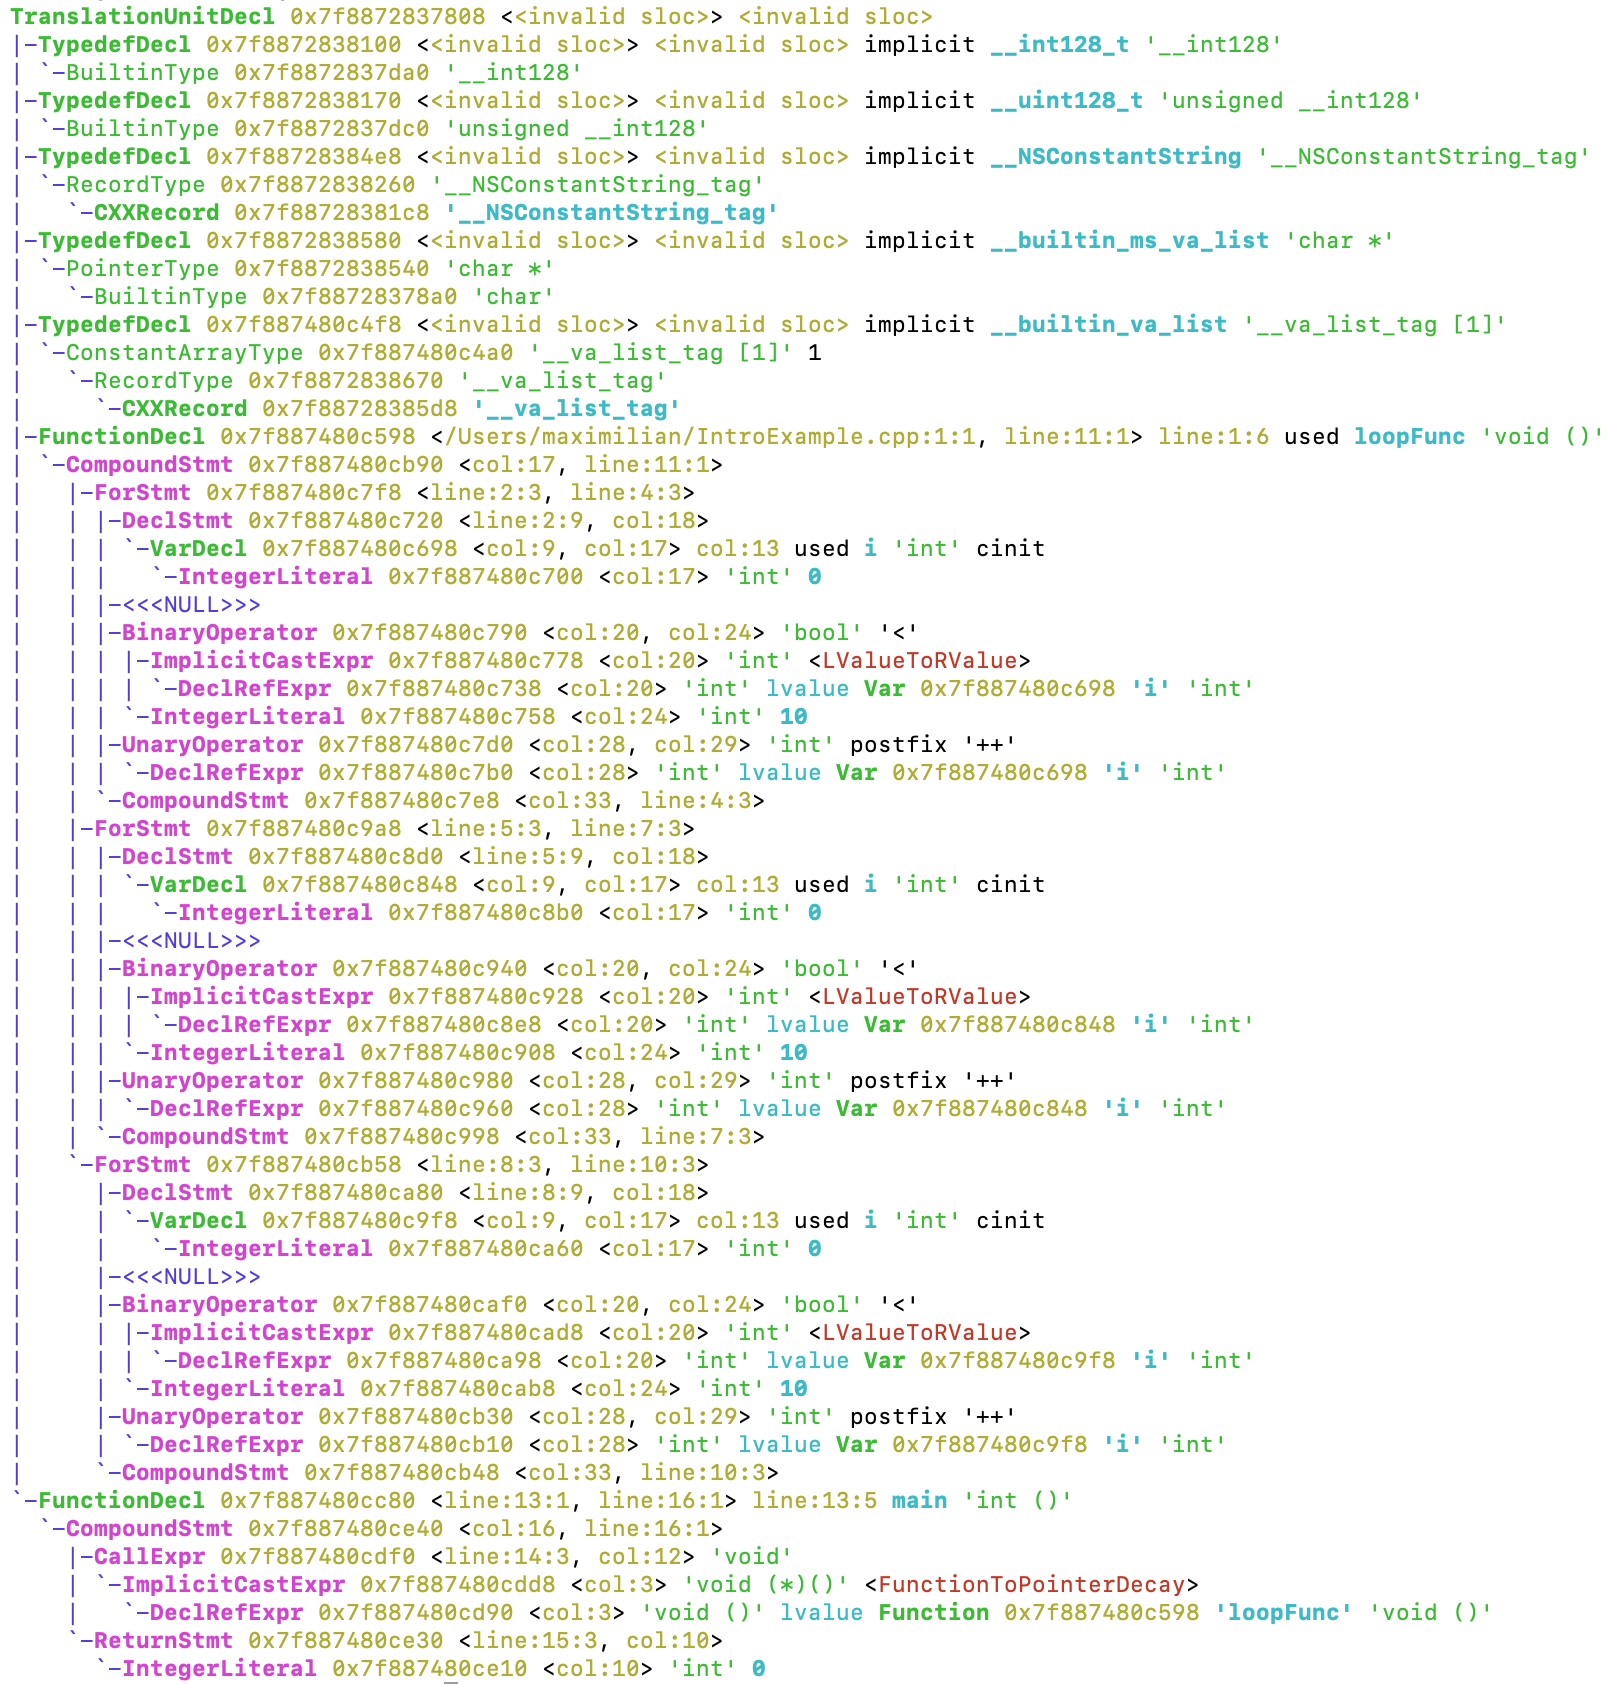
\includegraphics[width=1\textwidth]{graphics/t_ast.png}
  \label{fig:intro:dump ast example}
\end{figure}

To enable the user to develop his own tool based on the \CLANG framework, the so-called \lstinline{RecursiveASTVisitor} is provided. This contains a set of predefined functions and brings together all the information on how to access different \declssmall, \STATS and types. For instance, the method \lstinline{VisiteStmt(void)} provides a routine to traverse all the \STATS in the code. Users can access these interfaces to implement their own logic and perform \SOUTOSOU transformations. \CLANG's functions and existing infrastructure can thus be used to find places in an application and insert the desired code there~\cite{ClangLibTooling}. Therefore, the framework is very well-suited for writing an application that satisfies the objectives of the thesis. For the development of the tool we will use \LLVM version 14.0.1 and \CLANG version 14.0.1 built on top of it, also relying on the associated documentation~\cite{ClangDocs}.           % LLVM, Clang, AST
% Analysing %
\chapter{Analysis of the Abstract Syntax Tree}
\label{chapter3}
The aim is to develop a model that can efficiently analyze the \astsmall created by \CLANG for our type of application. The \TOOL is based on this concept. In order to be able to make modifications to a program code, we first have to take a closer look at the \astsmall of the input application. The analysis will focus on identifying the different node classes provided by \CLANG and how they can be categorized for our use case. We also need to look at how the positions for the performance counters can be found in the representation and what further modifications are necessary to insert the counters at the correct location. Finally, we need to find out how the program flow can be structured and whether it is possible to develop a recursive model that can be applied to all classes.

\section{Identification of the Core Classes}
In \CLANG, all instructions are grouped into the superclasses \declssmall, \STATS, and types. The core classes, which contain definitions for \declssmall and \STATS, are particularly interesting for our field of application, since many basic functionalities of a program can be represented with the instructions described in these classes. We will not discuss subclasses of the core class types any further, since we do not require information about the data types of the instructions in our type of application. In the following the classes provided by the \CLANG framework must be grouped and it must be analyzed how they are handled by the \TOOL. 

The \declssmall class contains, among others, the classes \lstinline{FunctionDecl} and \lstinline{VarDecl}. These classes are used to represent descriptions of functions and variables in the \astsmall. Listing~\ref{lst:c:ast_declstmt_code} shows a code snippet of a program in which a main function is defined that contains assignments to different primitive data types of \CPP. The corresponding \astsmall representation of \CLANG is shown in Figure~\ref{fig:c:ast_declstmt}. The information contained in the \lstinline{FunctionDecl} class is needed to get the content of a function. In the \TOOL, this data is used to get the content of the main function at the beginning of the analysis process and to handle function calls. If we look at the \DECL of a variable in more detail, we notice that the variable \DECL itself is grouped under the \lstinline{DeclStmt} class. Since we do not need to distinguish between the different data types for the insertion of measurement code, it is sufficient to examine the higher-level class \lstinline{DeclStmt} more closely. This class, however, is located in the core class \STATS. This superclass also contains all the other classes that we need to specify more. In particular, we are interested in the classes


\begin{lstlisting}[float, language=C++, caption=Example Code Showing the Definition of Functions and Variables., label=lst:c:ast_declstmt_code]
int main(void) {
    int integer = 1;
    char character = 'a';
    bool boolean = true;
    float floatingPoint = 1.1;
    double doubleFloatingPoint = 1.2;
}
\end{lstlisting}

\begin{figure}[t]
    \centering
    \caption{The \AST for \DECLS of Functions and Variables.}
    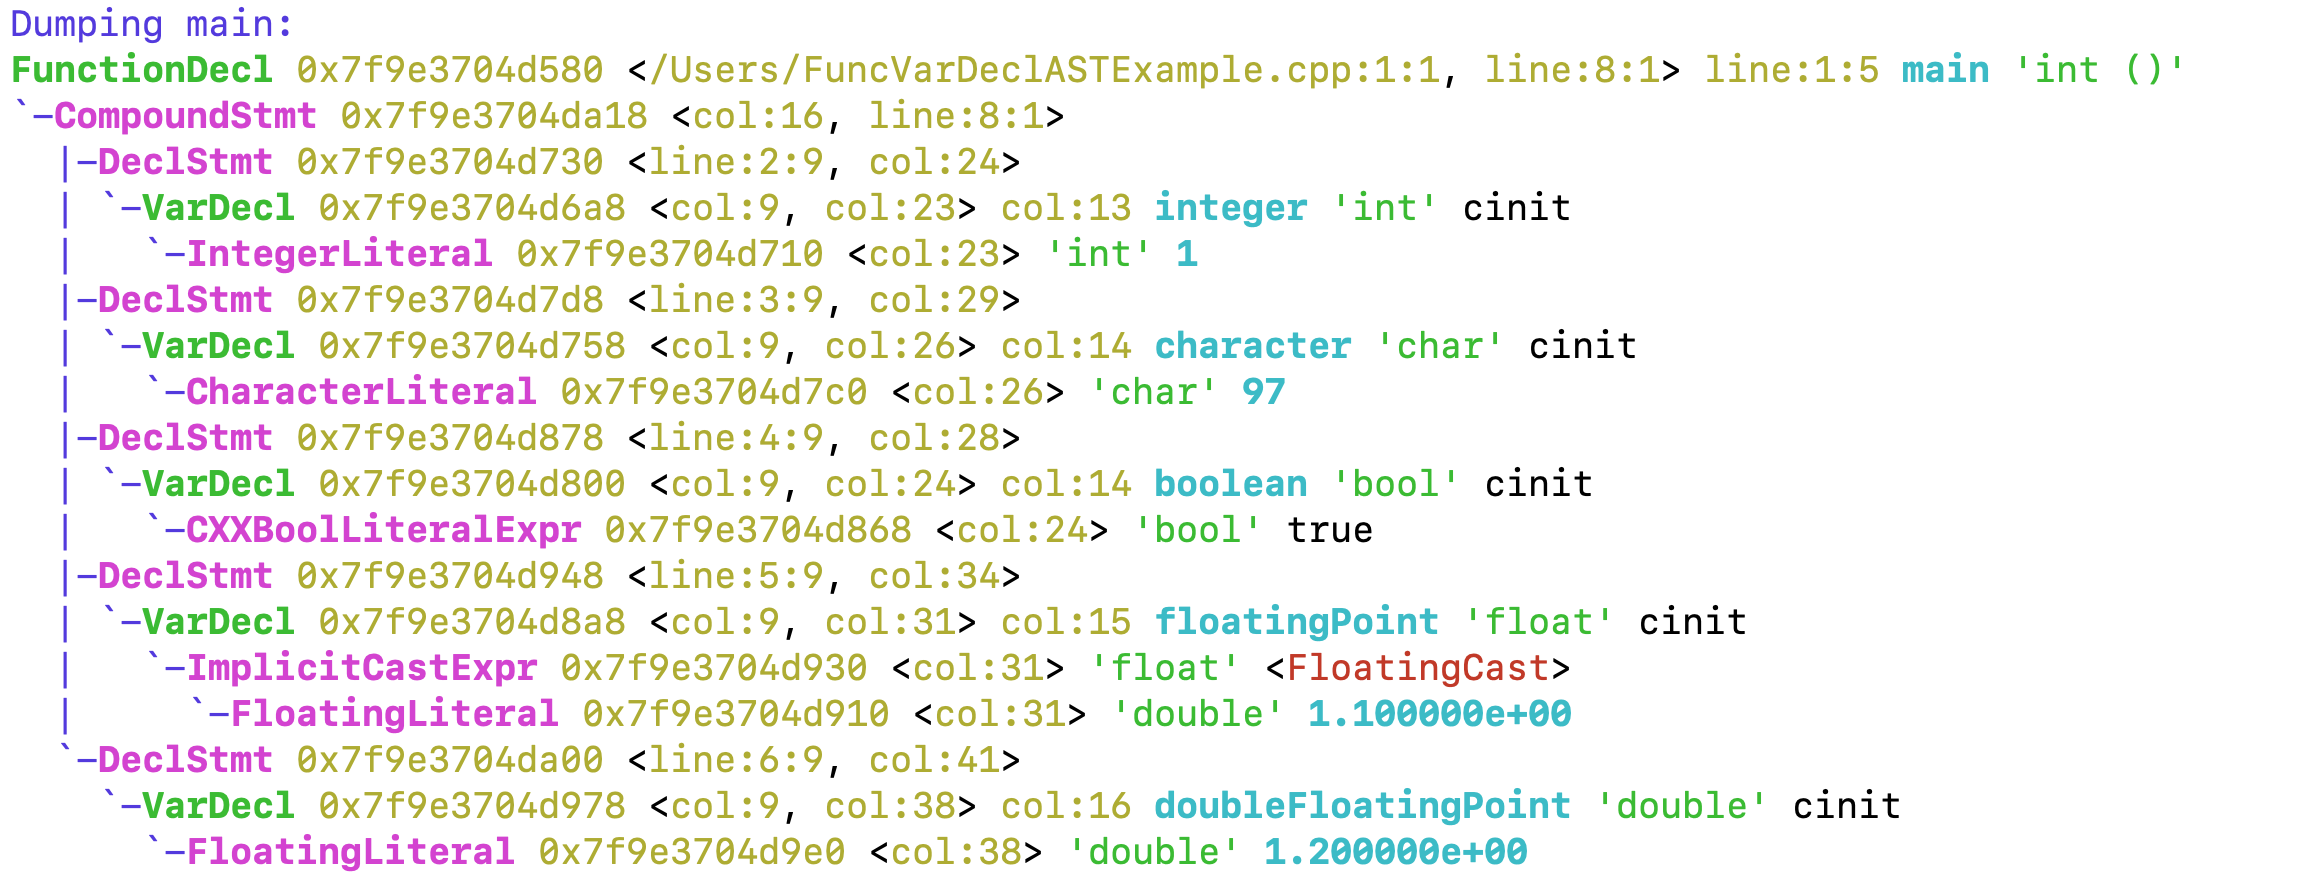
\includegraphics[width=1\textwidth]{graphics/c_ast_declstmt.png}
    \label{fig:c:ast_declstmt}
\end{figure}

\begin{itemize}[noitemsep, nolistsep]
    \item \lstinline{DeclStmt},
    \item \lstinline{OperatorCallExpr},
    \item \lstinline{BinaryOperator},
    \item \lstinline{CallExpr},
    \item \lstinline{CXXCallExpr},
    \item \lstinline{IfStmt},
    \item \lstinline{CaseStmt},
    \item \lstinline{ForStmt},
    \item \lstinline{DoStmt}, and
    \item \lstinline{WhileStmt}.
\end{itemize}

These classes were selected, since by describing these a variety of different programs can be analyzed by our transformation tool. These instructions provide basic functionalities which are used in each application and thus must be recognized by our profiler. We limit ourselves however in such a way that we do not have to identify each class which is made available by \CLANG, but address the most important classes mentioned before. 

\subsection{Leaf Nodes}
A group of \STATS is to be formed that contains operations that cannot be traversed further. We will call these instructions \LEASTAS. These include the frequently used classes \lstinline{DeclStmt}, \lstinline{OperatorCallExpr}, and \lstinline{BinaryOperator}. Nodes designated with the \lstinline{DeclStmt} class represent a variable \DECL. This operation can be neglected in the analysis of programs, since the runtime can be equated with a constant value. \lstinline{OperatorCallExpr} is used whenever an operator is called. For instance, this can occur when the software writes a value to a stream and outputs it. For nodes belonging to the \lstinline{BinaryOperator} class, two operands are used to get a result through a calculation or comparison. All three classes are examples of actions that are executed only once and cannot be further broken down into smaller parts. The group also contains other classes provided by the \CLANG framework that have similar characteristics. This group has the property that the \TOOL does not have to further traverse the instructions, but that measurement code can be directly be wrapped around them. 

\begin{lstlisting}[float, language=C++, caption=Example Code Showing the Definition of a Function Call., label=lst:c:ast_call_code]
void loopFunc() { 
    /* code block */ 
}

int main(void) {
    loopFunc();     // CallExpr Class
}
\end{lstlisting}

\begin{figure}[t]
    \centering
    \caption{The \AST for the \lstinline{CallExpr} Class.}
    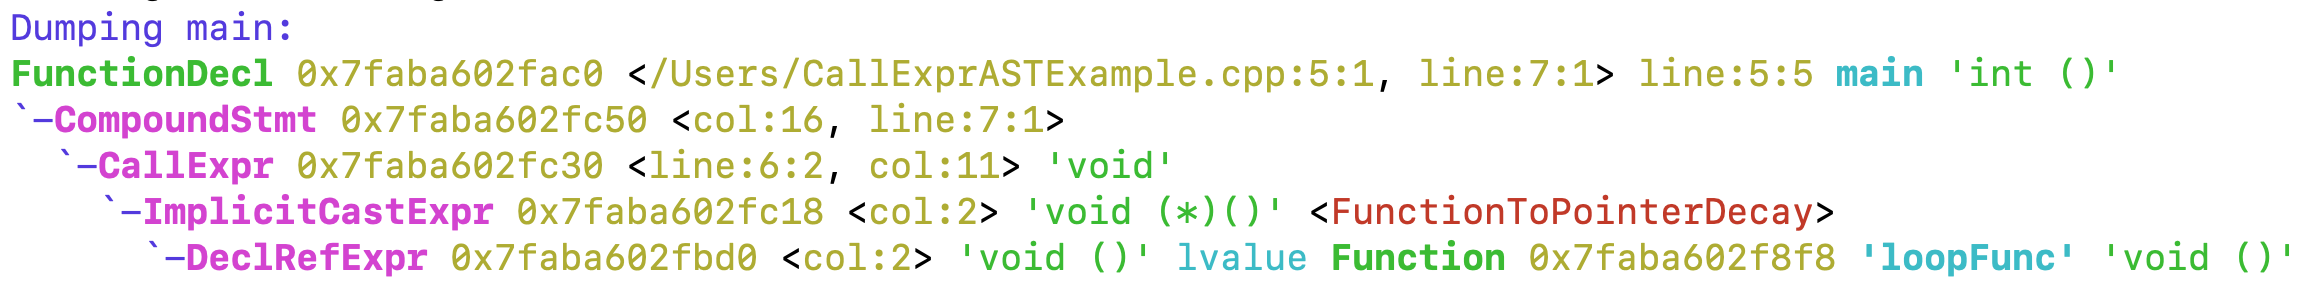
\includegraphics[width=\textwidth]{graphics/c_ast_call.png}
    \label{fig:c:ast_call}
\end{figure}

\subsection{Parent Nodes}
We will define all other classes in which we are interested in as \PARSTAS. These classes have the characteristics of an underlying layer that can also be traversed. They are of particular importance because we need to handle each special case of them separately. The code for a simple method call can be seen in Listing~\ref{lst:c:ast_call_code}. The corresponding representation in the \astsmall can be seen in Figure~\ref{fig:c:ast_call}, where the actual method call is specified by the class \lstinline{CallExpr}. In addition to the information about the location, this node also contains a reference to the function that is called. When the tool found this type of node it is necessary to check whether other nodes exist on the same level. If this is the case, the \PARSTA with all sub-levels can be enclosed as one unit with measurement code. If, however, there are no other siblings on this level, we must examine the subordinate level more closely. This is necessary because there would be no added value if only the runtime of a single possible resource-intensive class were output. In this case, we can use the \lstinline{getDirectCallee()} function provided by \CLANG to get the function that is called. For the class \lstinline{CXXMemberCallExpr} exactly the same approach can be applied.

\begin{lstlisting}[float, language=C++, caption=Example Code Showing the Definition of a Branch \STATLARGE., label=lst:c:ast_if_code]
int main(void) {
    int sum = 2;
    if(sum > 1)         { /* code block */ }
    else if(sum > 2)    { /* code block */ }
    else                { /* code block */ }
}
\end{lstlisting}

\begin{figure}[t]
    \centering
    \caption{The \AST for the \lstinline{IfStmt} Class.}
    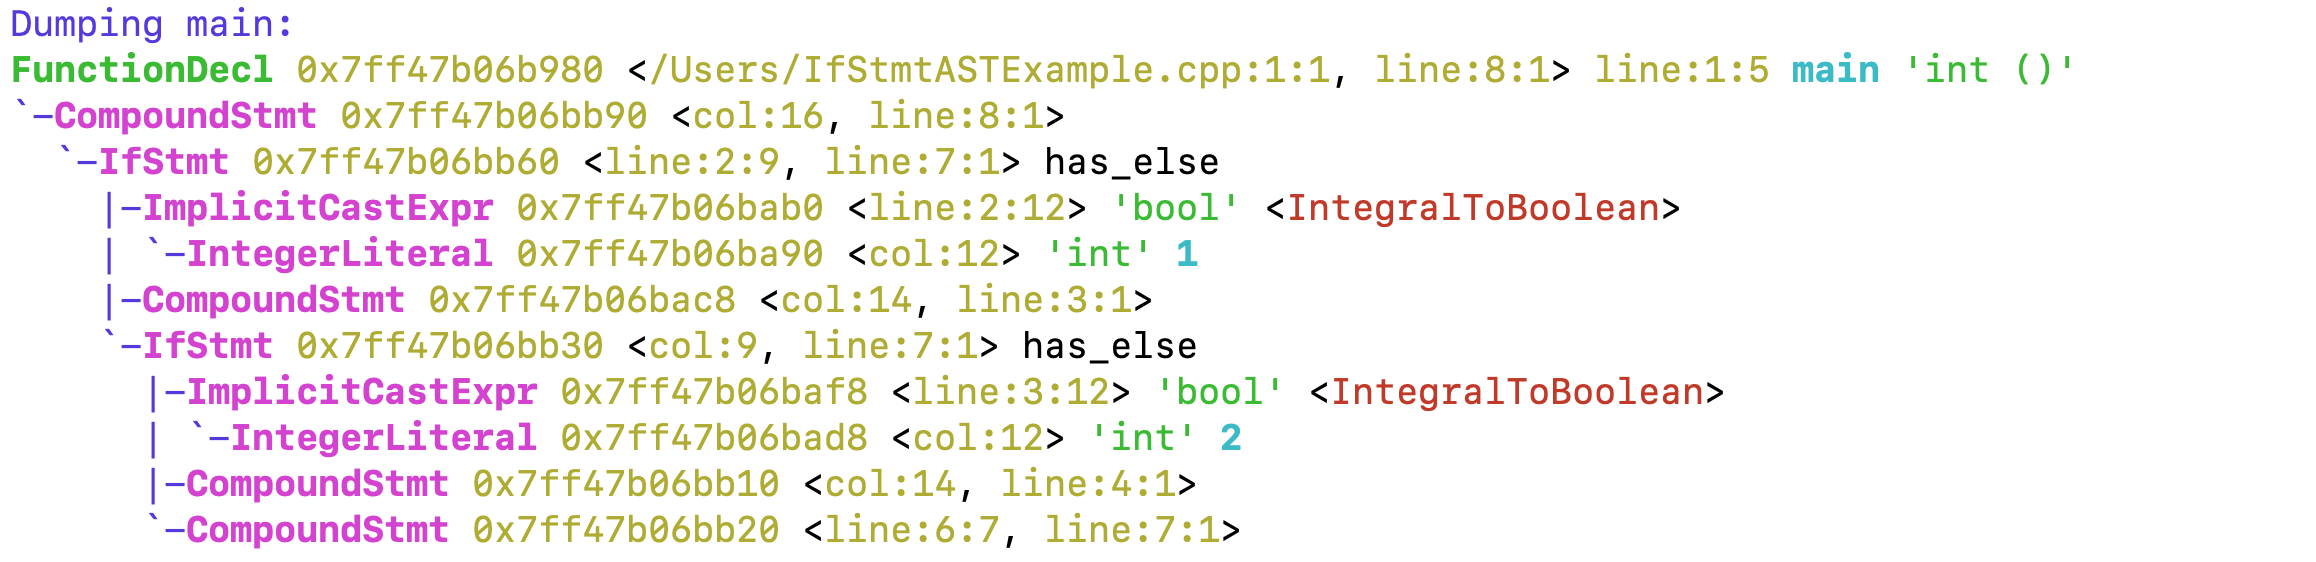
\includegraphics[width=\textwidth]{graphics/c_ast_if.png}
    \label{fig:c:ast_if}
\end{figure}

The code of a nested \lstinline{if-else}-query is shown in Listing~\ref{lst:c:ast_if_code}, with the associated \astsmall shown in Figure~\ref{fig:c:ast_if}. The first \lstinline{if}-\STAT represents the first query, whereas the nested \lstinline{if}-\STAT is actually an \lstinline{else-if}-branch. Both \lstinline{if}-\STATS have the \lstinline{has_else} flag, which means that there is an \lstinline{else}-branch in the query construction. To get the body of the \lstinline{if}-\STAT we use the \lstinline{getThen()} command. Once we have reached the last \lstinline{else-if}-branch, we check whether a flag labeled \lstinline{has_else} is set and in this case we can execute a \lstinline{getElse()} query. Nodes belonging to the Class \lstinline{CaseStmt} can be traversed analogously to \lstinline{if}-\STATS with the same method, but instead of the \lstinline{getThen()} function we use the \lstinline{getBody()} function.

\begin{lstlisting}[float, language=C++, caption=Example Code Showing the Definition of a Loop., label=lst:c:ast_for_code]
int main(void) {
    for(int i = 0; i < 10; i++) { /* code loop */ }
}
\end{lstlisting}

\begin{figure}[t]
    \centering
    \caption{The \AST for the \lstinline{ForStmt} Class.}
    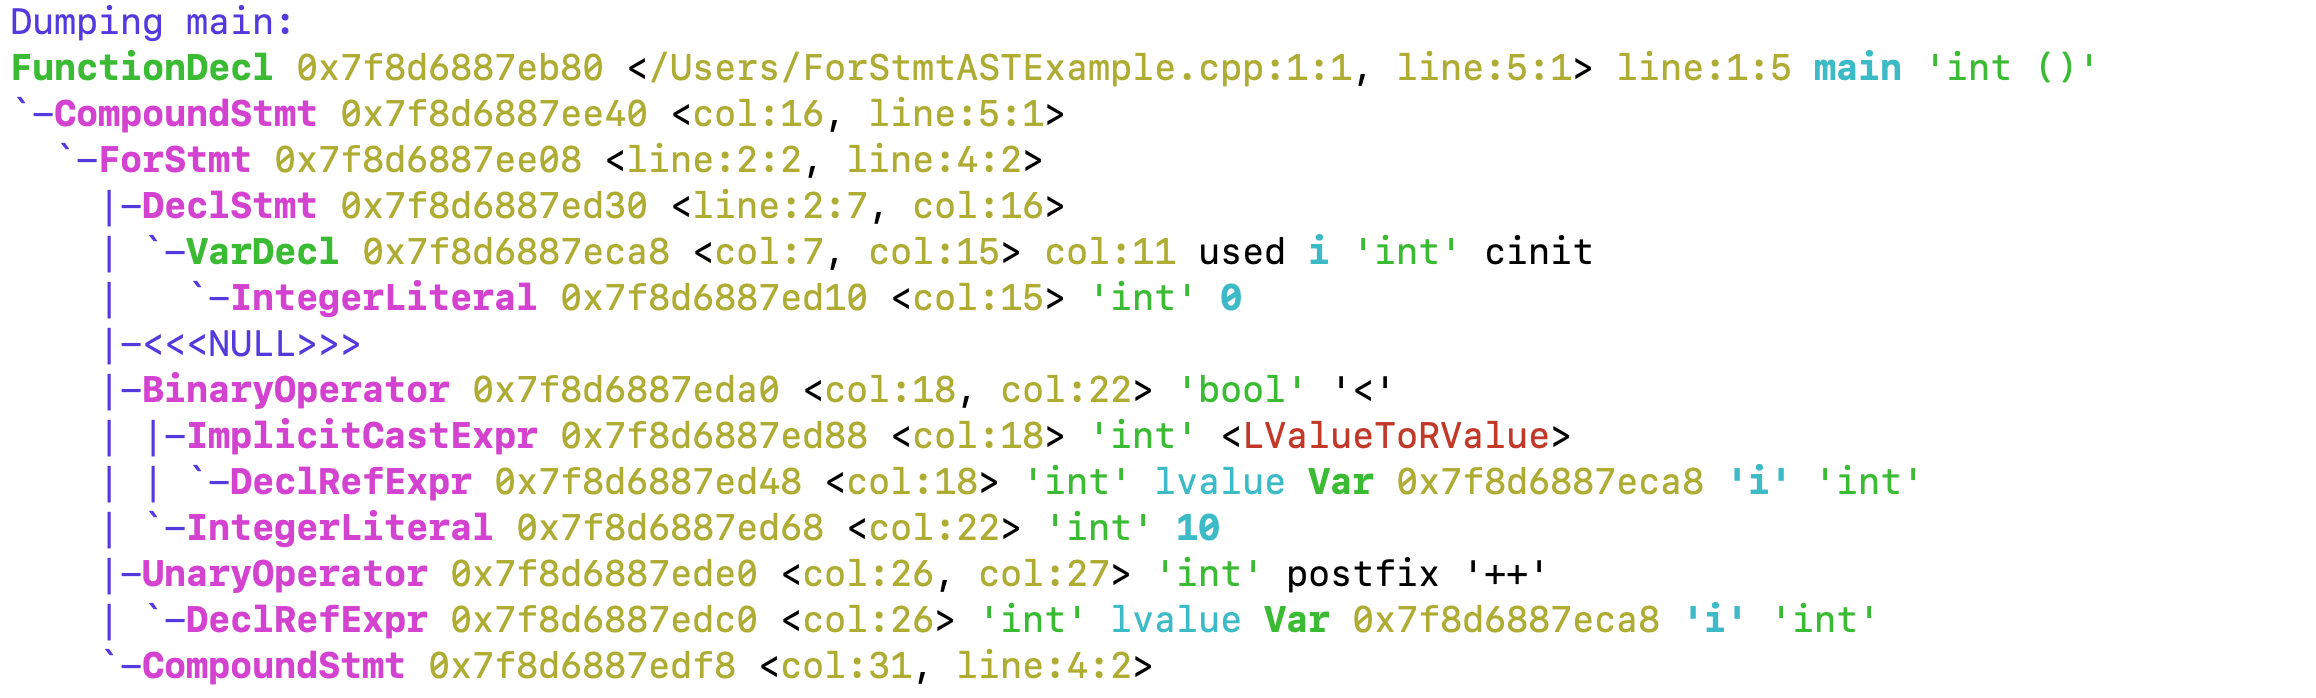
\includegraphics[width=\textwidth]{graphics/c_ast_for.png}
    \label{fig:c:ast_for}
\end{figure}

The implementation of a \lstinline{for}-loop, another \PARSTA that needs to be analyzed, can be seen in Listing~\ref{lst:c:ast_for_code}. The \astsmall generated from the code can be seen in Figure~\ref{fig:c:ast_for}. The analysis of loops is particularly complicated because the instructions in them can be executed several times. To get the content of the loop, we can simply use the function \lstinline{getBody()}, but the runtime calculation of the performance counter inserted there has to be taken into account. This is problematic because the inserted measurement code is called as often as the loop itself. The times of individual instructions must therefore be added together so that the total time of a \STAT can be calculated. The problem of the overhead generation will be discussed in more detail in Chapter~\ref{chapter5}. The process of traversing \lstinline{while}- and \lstinline{do/while}-loops can be treated analogously to that of \lstinline{for}-loops. It can thus be stated that \PARSTAS are only enclosed with performance counters if other elements exist on the same level. If this is not the case, the tool can immediately analyze the underlying level.

Furthermore, the \asts in Figure~\ref{fig:c:ast_call}, Figure~\ref{fig:c:ast_if}, and Figure~\ref{fig:c:ast_for} show nodes with the label \lstinline{CompoundStmt}. This is used to group children of a superordinate node. In the \lstinline{CompoundStmt} provided by \CLANG, however, there are nodes from both of the groups we identified. Instructions that belong to the group of \LEASTAS, including simple \declssmall of variables, should also be grouped together. To do this, however, classes that themselves contain further children must be removed and treated separately. For this purpose, we will create a separate class called \lstinline{CustomCompoundStmt} when traversing. For each node traversed, the tool checks which group it belongs to. If the current node is a \LEASTA, it is added to a \lstinline{CustomCompoundStmt} or a new \lstinline{CustomCompoundStmt} is initialized. A node of type \lstinline{CustomCompoundStmt} is closed when the first \PARSTA is reached. After this class has been handled separately, a new \lstinline{CustomCompoundStmt} can be initialized. This allows the runtime of all \LEASTAS to be combined. It should also be mentioned that this grouping is not done at runtime of the input program, but already in the analysis process of the tool, which reduces the resource consumption of the tool. 

\begin{lstlisting}[float, language=C++, caption=Fibonacci Application Example for Analysing the Identified Groups., label=lst:c:example_categorisation]
#include <iostream>

int fibonacci() {
    /* CustomCompoundStmt start */
    double n = 0;                               // leaf node
    t1 = 0;                                     // leaf node
    t2 = 1;                                     // leaf node
    nextTerm = 0;                               // leaf node
    n = 100;                                    // leaf node
    std::cout << "Fibonacci Series: ";          // leaf node
    /* CustomCompoundStmt end */

    for (int i = 1; i <= n; ++i) {              // parent node
        if(i == 1) {                            // parent node
            /* CustomCompoundStmt start */
            std::cout << t1;                    // leaf node
            std::cout << ", ";                  // leaf node
            /* CustomCompoundStmt end */
        }
        else if(i == 2) {                       // parent node
            /* CustomCompoundStmt start */
            std::cout << t2;                    // leaf node
            std::cout << ", ";                  // leaf node
            /* CustomCompoundStmt end */
        }
        /* CustomCompoundStmt begin */
        nextTerm = t1 + t2;                     // leaf node
        t1 = t2;                                // leaf node
        t2 = nextTerm;                          // leaf node
        std::cout << nextTerm << ", ";          // leaf node
        /* CustomCompoundStmt end */
    }
}

int main(void) {
    fibonacci();                                // parent node
    return 0;
}
\end{lstlisting}

\subsection{Classification Approach by Example}
The collected knowledge about the classes of the nodes can now be used to analyze the example code, shown in Listing~\ref{lst:c:example_categorisation}, of an application that calculates the first hundred Fibonacci numbers. In order to better understand the procedure of the \TOOL, we will also start traversing the nodes in the main function. In the first line of the main function, a function call can be seen, which can be classified as a \PARSTA, since the sub-tree of the function \DECL can be accessed by calling this function. In the first sub-level of the function \DECL, there are first six instructions that can be marked as \LEASTAS, since no further levels can be reached through these nodes. Furthermore, these instructions can be combined as \lstinline{CustomCompoundStmt}, as the individual runtimes will be negligible. Next, there is a \lstinline{for}-loop that must be declared as a \PARSTA, since further instructions are called from it. The two \lstinline{if}-instructions found in the level below also contain children and are therefore also defined as \PARSTAS. Each instruction contains two simple instructions that can declared as \LEASTA and grouped together as \lstinline{CustomCompoundStmt}. At the end of the function there are four more instructions that are also marked as \LEASTAS and can be combined. It should be noted that in the actual traversal process not all levels are annotated at once. If the \TOOL is executed without further options, only the content of the \lstinline{fibonacci()} function would be annotated for the time being. With the information gained from the first run, the user can specify a desired region to be looked at in more detail. 

Finally, it can be stated that the nodes of the \astsmall can be divided into two groups for our purposes. \emph{Leaf nodes} that are summarized as \lstinline{CustomCompoundStmt} and \PARSTAS that have to be considered separately. For groups of \LEASTAS, only one shared runtime is calculated by the \TOOL. \emph{Parent nodes} are tracked individually if other instructions exist on the same level. If only one superclass is found on the currently examined level, its content is analyzed in more detail. If the special case occurs that each level contains only one instruction, only the total runtime of the program is calculated and output, as no detailed profiling statistic can be provided for the input application. 

\section{Detection of the Insert Locations}
In order to insert the measurement code in the right places, we need information about the positions of the nodes in the actual program code. These are stored in the \SOUMNG of the \astsmall and can be accessed by calling functions of the \CLANG infrastructure. For the \TOOL, functions that access the first and last location of the node are particularly important. However, the results of these predefined functions must be modified. If we now use the functions to obtain the boundary positions of a node and insert our measurement code into them, we get an output that looks similar to the code shown in Listing~\ref{lst:c:insertion_lexer}. It can be seen that the example code was inserted correctly before the instruction under consideration, but the end tag differs from the desired result. To generate code that creates the desired result, the code must be inserted after the closing curly brace. However, the locations obtained with the \lstinline{getBeginLoc()} function can be used immediately to insert the code at these locations. 

\begin{lstlisting}[float, language=C++, caption=Wrong Insertion Position When Using End Location of Node., label=lst:c:insertion_lexer]
void loopFunc() {
    startEvent(1);          // getBeginLoc() returns the correct position
    while ( i <= 10 ) { 
        i++; 
        endEvent(1);        // getEndLoc() returns the incorrect position
    }
    /* "endEvent(1);" should be inserted at the position after the brace */
}
int main(void) {
    startEvent(0);
    loopFunc();
    endEvent(0);
    print();
    return 0;
}
\end{lstlisting}

The function \lstinline{getEndLoc()}, on the other hand, does not return the first place after the examined node, but the last place in it. As can be seen in Listing~\ref{lst:c:insertion_lexer}, this leads to the measurement code not correctly enclosing the node. If the instruction does not contain opening and closing brackets, the position before the semicolon may also be returned. Both problems can be solved analogously. The solution is to develop a function that checks the current token and moves the position with the information obtained. To do this, first check whether the token at the current position is of type \lstinline{clang::tok::semi} or of type \lstinline{clang::tok::r_brace}, which allows the parameters for subsequent actions to be determined. Afterwards, the interface \emph{Lexer} provided by \CLANG, which allows certain actions on the streams of tokens, can be used to find the desired position with the function \lstinline{Lexer::FindLocationAfterToken()}. This method takes the current token and the character to be searched for and returns the position after the first character searched for. Finally, we can state that the start position and the end position of all nodes are now returned correctly for our purposes. With these positions, the measurement code can be wrapped around different groups of nodes. 

\section{Application of a Recursive Model to the Core Classes}
\begin{figure}[p]
    \centering
    \caption{Flow Chart Representing the Logic of the \TOOL.} 
    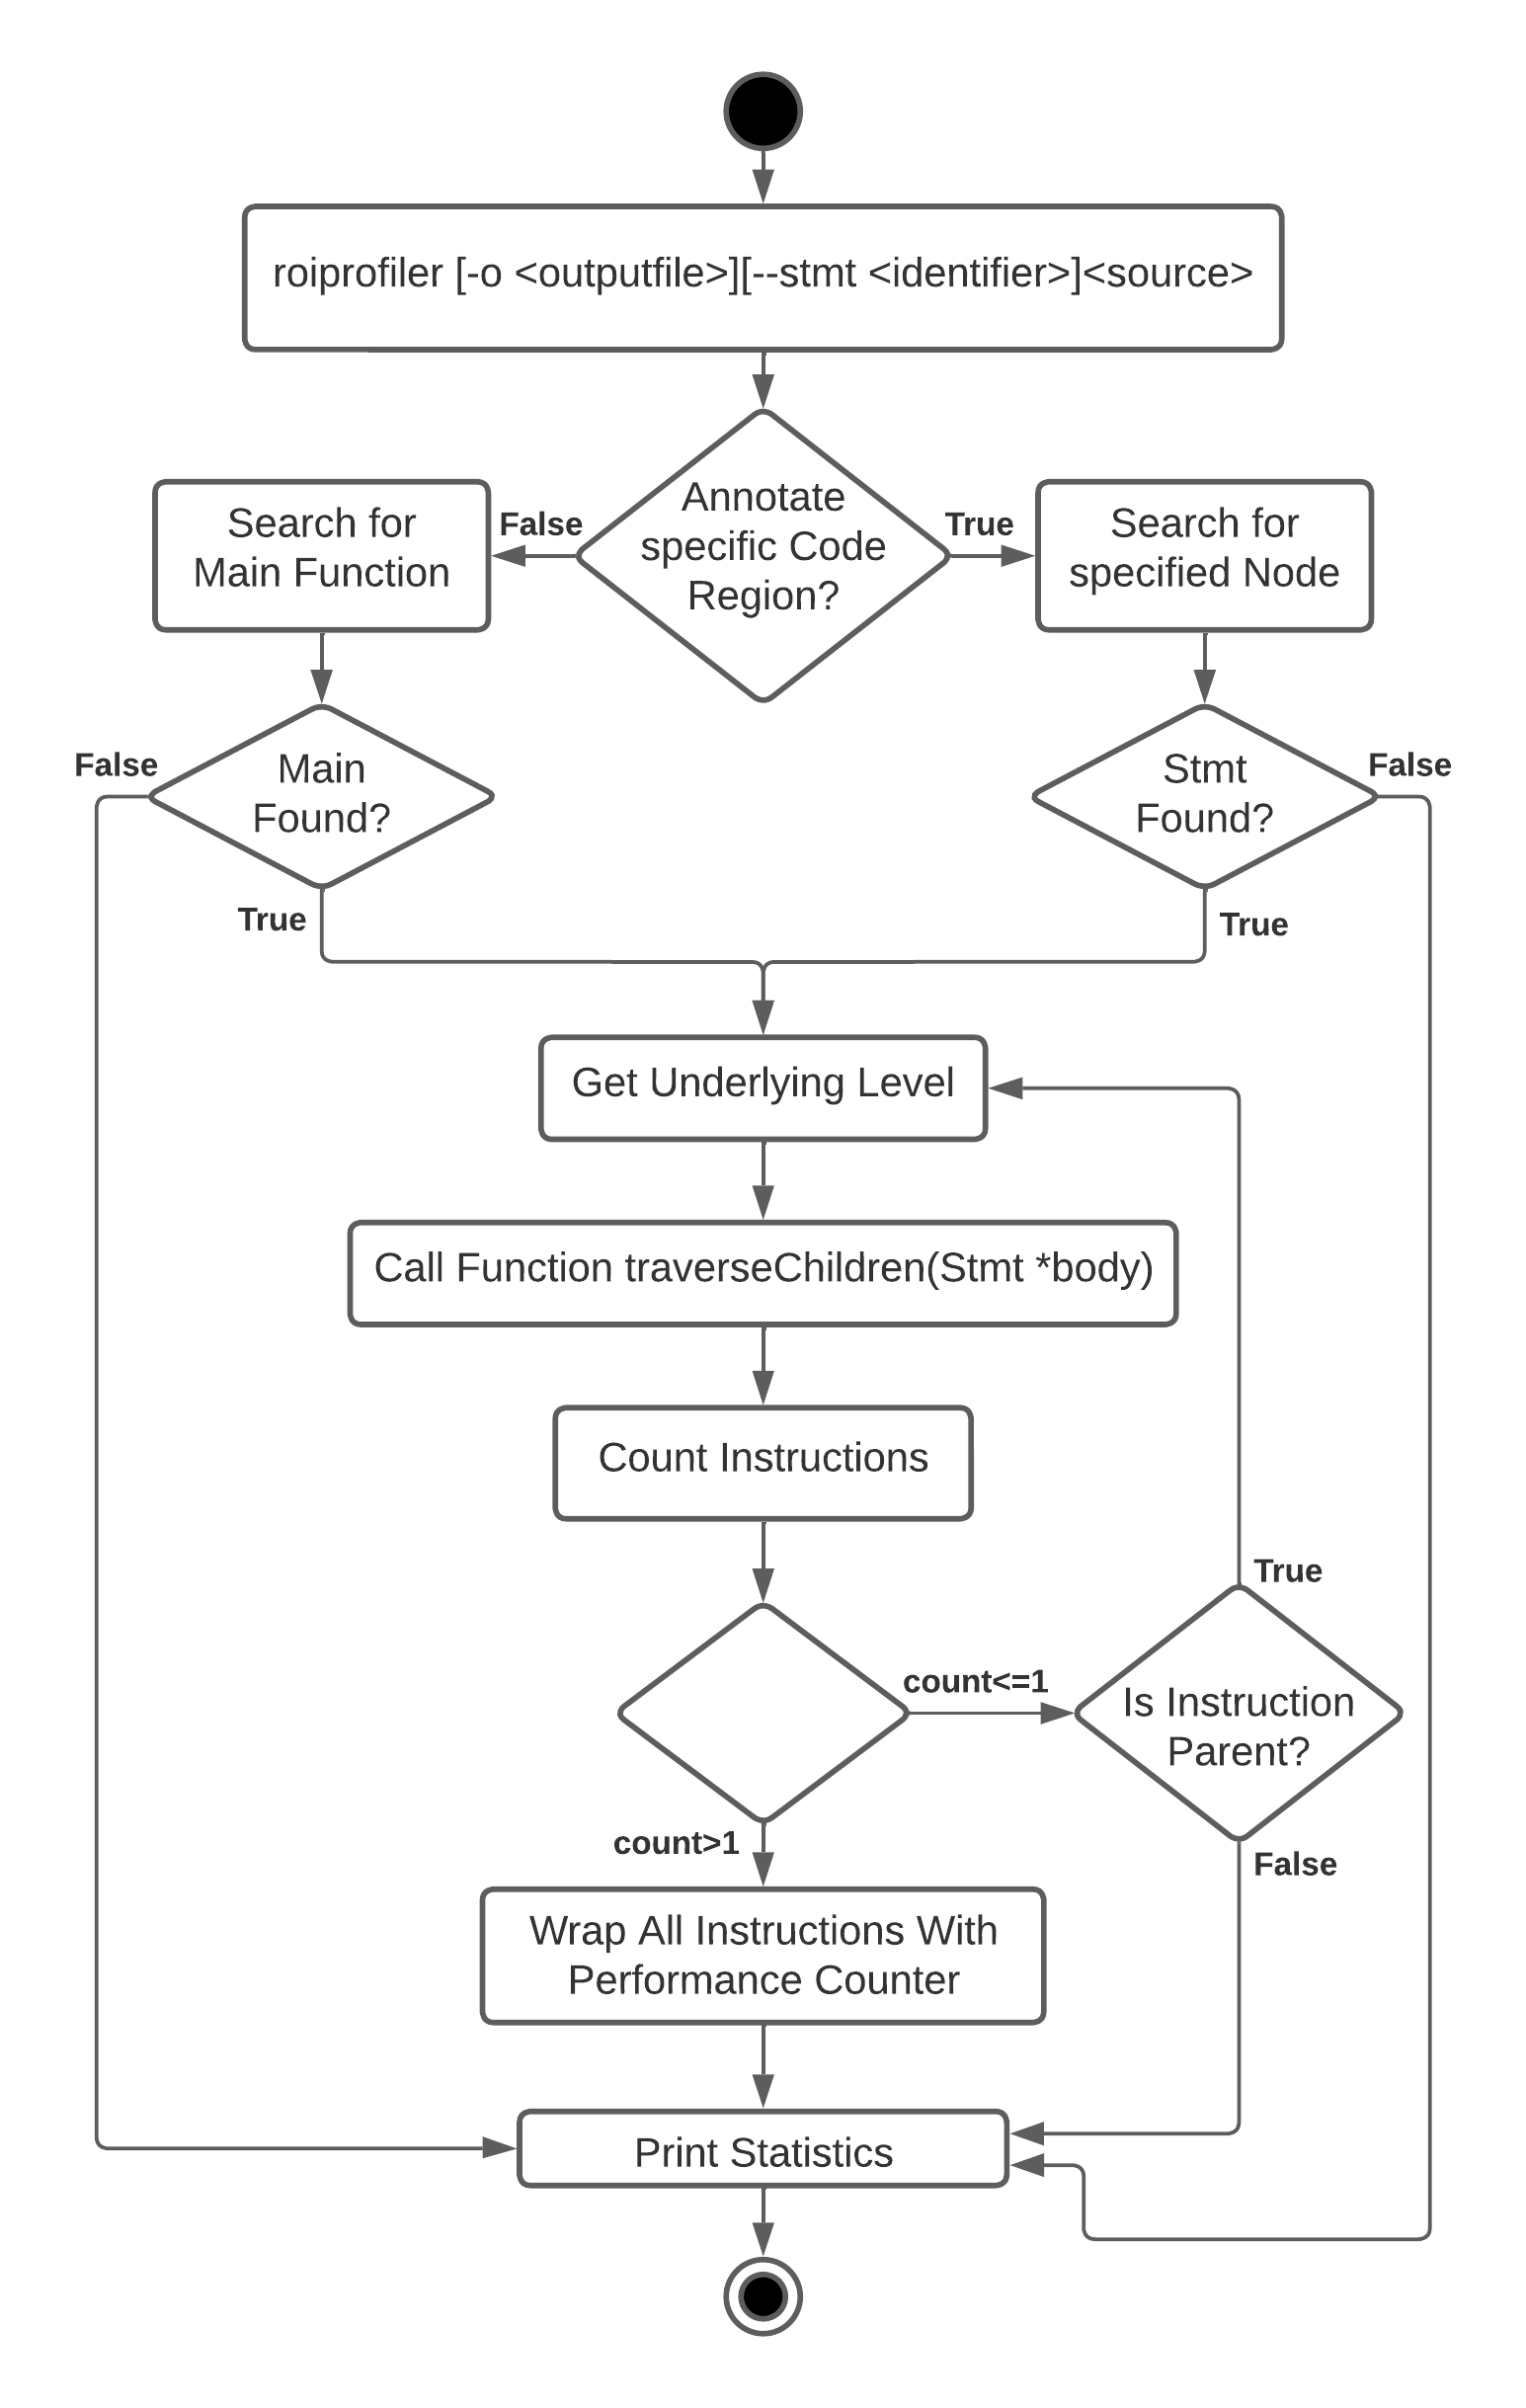
\includegraphics[width=.75\textwidth]{graphics/c_flow_chart.png}
    \label{fig:c:flow_chart}
\end{figure}

In the following we discuss the flow of the \TOOL and explain how all the different types of nodes can be traversed recursively. For this purpose, the input parameters and the expected output of the \TOOL should be defined first. As a mandatory input parameter, the \TOOL should accept a source code written in \C /\CPP. The storage location for the transformed program can be specified optionally. Furthermore, the user can decide in which \roismall instructions are to be annotated. At the beginning of the profiling process, the \TOOL should wrap all code blocks of the main function with performance counters and return transformed software that can be executed by the user. In addition to the actual output of the input program, the user is provided with useful feedback on the resource consumption of individual instructions in the main function. Each instruction that supports a more detailed analysis is shown with an identification number. The user can utilize these identifiers to start the next iteration of the analysis by specifying desired regions and launching the \TOOL again. 

Now that the basic characteristics of our tool are known, the logic of the process behind it can be analyzed. A flow diagram of the simplified process is shown in Figure~\ref{fig:c:flow_chart}. The process is started by calling the \TOOL with the correct parameters. The first step is to check which mode is currently active and, depending on this, either search for the \ENTPOI to the input application or search for an instruction specified by the user. In both cases, the source code created by \CLANG is first searched for the desired node. The \TOOL is terminated if neither a main function nor a node with the searched identifier is found. If the search is successful, the node found of the instruction is passed to the \lstinline{traverseChildren(Stmt*)} function. Further, the content of the passed node is taken so that the child nodes can be counted and categorized. The number of children is needed to make a basic case distinction. If several nodes are located at this level, they can be annotated and the program can be terminated. However, if only one node is found at this level, it must be checked whether it belongs to the group of \PARSTAS. The special case of only one instruction occurring in each level is achieved if the node is not a \PARSTA. In this case, only the runtime of the entire application is returned, as no analysis of individual instructions is possible. However, if the \TOOL detects another level that can be analyzed, the content of the \PARSTA can simply be forwarded recursively. 

In the process shown in Figure~\ref{fig:c:flow_chart}, it can be stated that all properties for the development of a recursive method apply. In general, the overarching problem is to examine all levels of the \astsmall and to assign performance counters to certain sub-areas. The sub-problem is to examine a single level of the tree and to examine nodes on this level. Furthermore, the \TOOL has two base cases that serve as termination conditions. One is met when multiple nodes at a level are found, in which case we can simply annotate them all and solve the problem. The other termination condition is given if only one \LEASTA exists which has no other levels below it. If there is only one instruction on a level that has other child nodes, we can simply traverse that level by calling the function itself. This procedure is repeated until either all levels have been traversed, or until a level has been found that can be annotated and the overall problem has been solved. This is very useful, since it is not necessary to consider each level separately, or even to count the depth of the \astsmall at the beginning. Thus, it makes no difference how many levels are below the starting point, as the program only terminates after the last level has been reached. 

\subsection{Traversing Approach by Example}
Based on this method, the example code shown in Listing~\ref{lst:c:example_traverse} can now be analyzed. When the traversal process begins, the main function is searched for and checked to see how many instructions have been specified in it. In this case, the main function contains only one instruction of the type \lstinline{CallExpr} (\lstinline{loopFunc()}). Since a node was found that has subordinate levels, the contents of this can be passed on to the \lstinline{traverseChildren(Stmt*)} function. Subsequently, the children of this node are also examined, but this time an instruction of the class \lstinline{ForStmt} is present. This class also falls into the group of \PARSTAS and the content must therefore be traversed again. On the next level, it is noticeable that not only one \LEASTA is to be executed. The termination condition is reached and all nodes on this level can be wrapped with performance counters. If we change the example a little and give the tool the identifier of the \lstinline{for}-loop in the \lstinline{loopFunc()} function as the starting point, all previous steps would be skipped by the \TOOL and the body of the \lstinline{for}-loop can be annotated immediately. With the insertion of the performance counters, the first run of the profiling process is finished, and the user now has the option of running the \TOOL again with the identifiers of the \lstinline{while}-loops to start a more detailed analysis of them.

\begin{lstlisting}[float, language=C++, caption=Example of the Model Used to Traverse the \AST., label=lst:c:example_traverse]
void loopFunc() {
    // children.size() <= 1 && child.getClass() == Stmt::ForStmtClass
    // // => traverseChildren(child.getBody())
    for (int i = 0; i < 10; i++) {
        // children.size() > 1 
        // => annotate all instructions
        for { /* code loop 1 */ }
        for { /* code loop 2 */ }
        for { /* code loop 3 */ }
    }
}

int main(void) {
    // children.size() <= 1 && child.getClass() == Stmt::CallExpr
    // => traverseChildren(child.getBody())
    loopFunc();                                            
}
\end{lstlisting} 

Finally, it can be stated that a model was found with which all classes of the group of \PARSTAS can be treated equally. After the categorization of the nodes, depending on the class type, it can be determined how the underlying \lstinline{CompoundStmt} class can be accessed. If access is gained to this node, it can be passed on as a node of the superclass \lstinline{Stmt} as a parameter to the \lstinline{traverseChildren(Stmt*)} function. The fact that the node can be represented as a \lstinline{Stmt} is particularly important, as all the functions necessary for our purpose can be accessed. From this point on, the procedure is the same for all classes. It can therefore be said that when applying this model, it makes no difference which type of \PARSTA is to be traversed. This is very useful, as a single recursively defined function is sufficient to traverse the sub-levels of all class types.
        % Analysing AST, Core Classes, Locations, Recursive Model
% Transformation %
\chapter{Source-to-Source Transformation and Outcome Visualization}
\label{chapter4}
\CLANG provides another library called \LIBTOOLING which, in addition to accessing the \astsmall, also provides predefined functions and classes that can be used to traverse a program structure and perform a \SOUTOSOU transformation. In Chapter~\ref{chapter3} we looked at analyzing the structure of a program in which performance counters are to be inserted. In addition, the fundamental procedure of the profiling process was discussed. Thus, we have analyzed all the theoretical considerations and laid the foundation for the development of the \TOOL, which is the focus of this Chapter. For this purpose, we first look at which actions are provided by \CLANG and how these can be used to write our own application. Furthermore, we explore how the measurement code can be inserted efficiently and how the overhead can be reduced by performing resource-intensive operations before the actual execution of the application to be profiled. For the calculation of the runtimes and the output of the data, a library is introduced that can be customized by the user. Finally, we discuss the workflow of the profiling process.

\section{Utilization of the Clang Infrastructure}
In addition to the \astsmall provided, which is enormously valuable for our purpose, \CLANG also provides a library that allows users to develop their own front-end compiler actions~\cite{ClangTooling}. Since some of the functions provided by the library simplify the development of our \SOUTOSOU transformation application, we will use them. In the previous section, we already discussed the basic characteristics of the \TOOL. These can now be specified in more detail, so that the basic structure of the application can be created. In Listing~\ref{lst:b:clang_options}, it can be seen that we give the tool the name ``\emph{roiprofiler}'' by creating an \lstinline{llvm::cl::OptionCategory}.

\begin{lstlisting}[float, language=C++, caption=Code Showing Option Definitions for Creating a \CLANG Tool., label=lst:b:clang_options]
/* Definition of the Tool Name */
static llvm::cl::OptionCategory MyToolCategory( "roiprofiler options" );

/* Specification of the Output File Option */
static cl::opt <string> OutputFile( "o", 
           cl::desc( "Write transformed file to custom location" ),
           cl::value_desc( "output file" ), 
           cl::cat( MyToolCategory ));

/* Specification of the Statement Option */
static cl::opt <string> Statement( "stmt", 
    cl::desc( "Specifies the current traversal point" ),
    cl::value_desc( "id of stmt" ), 
    cl::cat( MyToolCategory ));


int main( int argc, const char **argv ) {
    /* Bind the Specified Options to the Tool */
    auto ExpectedParser = CommonOptionsParser::create( 
                              argc, argv, 
                              MyToolCategory, 
                              llvm::cl::Required );
}
\end{lstlisting}

Furthermore, we will create two variables of the class \lstinline{cl::opt}, which represent the parameters of the \TOOL. It is necessary to mention that we do not have to explicitly specify that one of the input parameters is a source code of an application, as all \LIBTOOLING tools require this property. However, we do need to indicate that the output location may be set with the \lstinline{-o}~option. Furthermore, we specify that the starting point of the traversal can be set by the user with the option~\lstinline{--stmt}. The final step is to create a common option parser in the main method of the tool, which contains the specified options. Once an executable program has been created from the code, it is possible to run it in the \CLANG environment, as shown in Figure~\ref{lst:b:tool_synopsis}.

After the basic properties of the program have been defined and the \TOOL has been registered in the \CLANG environment, it is now possible to consider how a front-end action can be built with the infrastructure provided. The \ENTPOI for this is the \lstinline{FrontendAction} interface, with which custom actions can be executed on the code. A new \lstinline{FrontendAction} can be implemented using the \lstinline{Tool.run(newFrontendActionFactory)} instruction. Then the classes provided by \CLANG can be overwritten. The \CPP syntax for including the framework provided by \CLANG is shown in Listing~\ref{lst:b:clang_libtooling}. Next, the created front-end action is used to create an \lstinline{ASTConsumer} for each traversion unit. This allows the \astsmall to be accessed programmatically. For our scope, we will now call the function \lstinline{TraverseDecl} in the class \lstinline{Visitor}. We give this function the top level node of the \astsmall as a parameter, which allows us to determine the \ENTPOI of the traversal. By calling this function, all nodes of the \astsmall are visited. Finally, the \lstinline{RecursiveASTVisitor} can be used to visit selected nodes of different classes. In the constructor of the \lstinline{Visitor}, a reference to the \SOUMNG must be created, this will be important later for inserting the measurement code. The class \lstinline{RecursiveASTVisitor} can utilize a variety of different functions to traverse the different node types. For our purpose, we need the functions \lstinline{VisitFunctionDecl(FunctionDecl *func)} and \lstinline{VisitStmt( Stmt *stmt )}. The former iterates over all definitions of functions in the code, which is needed to annotate the instructions in the main function if no \lstinline{--stmt} option is given, and to insert performance counters that measure the runtime of the entire application. The \lstinline{VisitStmt( Stmt *stmt )} function is needed to look for \STATS in the code that have been specified by the user. From this point on, the recursive model developed can be used to traverse each level of the \astsmall. 

\begin{lstlisting}[float, language=C++, caption=The Synopsis of the \TOOL.,basicstyle=\footnotesize\ttfamily\tiny, label=lst:b:tool_synopsis]
sh-3.2# roiprofiler -help
USAGE: roiprofiler [options] <source0> [... <sourceN>]

OPTIONS:

Generic Options:

--help                          - Display available options
--help-list                     - Display list of available options
--version                       - Display the version of this program
    
roiprofiler options:

--extra-arg=<string>            - Additional argument to append to the compiler command line
--extra-arg-before=<string>     - Additional argument to prepend to the compiler command line
-o=<output file>                - Write transformed file to custom location
-p=<string>                     - Build path
--stmt=<id of stmt>             - Specifies the current traversal point
\end{lstlisting}

\begin{lstlisting}[float, language=C++, caption={[Framework for Accessing the \AST Provided by \CLANG.]Code Framework for Accessing the \AST Provided by \CLANG.}, label=lst:b:clang_libtooling]
/* Definition of the RecursiveASTVisitor provided by Clang */
class Visitor : public RecursiveASTVisitor<Visitor> {
private:
    ASTContext *astContext;
public:
    explicit Visitor( ASTContext *Context ) : astContext( Context 
    {
        rewriter.setSourceMgr( astContext->getSourceManager( ),
                               astContext->getLangOpts( ));
    }

    /* Functions for traversing the AST */
    virtual bool VisitStmt( Stmt *stmt ) {}
    virtual bool VisitFunctionDecl( FunctionDecl *func ) {}
    virtual ~Visitor( ) { }
};

/* Definition of the AST Consumer */
class Consumer : public ASTConsumer {
private:
    Visitor Visitor;

public:
    explicit Consumer( ASTContext *Context ) : Visitor( Context ) { }

    virtual void HandleTranslationUnit( ASTContext &Context ) 
    override { Visitor.TraverseDecl( Context.getTranslationUnitDecl( )); }
};

/* Definition of our frontend action */
class ClangFrontendAction : public clang::ASTFrontendAction {
public:
    virtual std::unique_ptr <clang::ASTConsumer>
    CreateASTConsumer( clang::CompilerInstance &Compiler, 
                       llvm::StringRef InFile ) 
    override { return std::make_unique<Consumer>( 
               Compiler.getASTContext( )); }
};

int main( int argc, const char **argv ) {
    /* Creation of a new frontend action */
    int result = Tool.run( 
                    newFrontendActionFactory<ClangFrontendAction>( ).get( ));
}
\end{lstlisting}

\section{Insertion of Callback Functions}
The in Chapter~\ref{chapter3} gathered knowledge about locating the different regions can now be used to insert measurement code. At the first accessible point in the source code, we will import the library needed to calculate the runtimes. Furthermore, the self-developed library \DATA, which will be described in more detail later, is imported and initialized. All nodes for which performance indices are to be measured must be enclosed with performance counters. For each region, two positions are needed, one before and one immediately after the region. Before each region, the function \lstinline{startEvent(int identifier)} should be called, and after it, the function \lstinline{endEvent(int identifier)} should be called. To transform the input application, the interface \lstinline{Rewriter} can be used. If we initialize this class, we get the possibility to use the function \lstinline{InsertText(SourceLocation Loc, StringRef Str)} to modify the source code. Since we already know the correct locations of the instructions, we only need to make sure that they are forwarded to the function. In addition to the position in the source code, the code to be inserted must also be specified. This function is always called when the position before or after a node to be annotated is reached. If a single node, such as a \PARSTA or a stand-alone \LEASTA, is to be annotated, the start and end positions can simply be determined. The \lstinline{startEvent(int identifier)} function is then inserted at the start position, and the \lstinline{endEvent(int identifier)} function at the end position. If several nodes are combined into a \lstinline{CustomCompoundStmt}, the start position is noted when the first node is visited and the end position when the last node is reached. The two functions can now be inserted at the positions found. Furthermore, it should be noted that the entire main class is enclosed with measurement codes and, if necessary, the runtime of a selected scope is also measured. Finally, after the last \STAT in the main class, a function \lstinline{print()} is added, which is responsible for the output of the collected measured values. 

Listing~\ref{lst:b:transformed_file} shows an example of how the transformed code looks with the measurement code inserted. It can be seen that the \DATA library is included and can already be filled with data from the annotated nodes during initialization. In this case, both the total runtime and the runtime of the desired region are measured. Within the region there are four \LEASTAS, whereby two can be combined in a \lstinline{CustomCompoundStmt} class. Furthermore, the three \lstinline{while}-loops are annotated. Finally, the \lstinline{print()} method is called as the last \STAT, which outputs the collected data in a table. Thus, it can be stated that all functions needed for the calculation of the performance have been inserted in the correct~places.

The \DATA library was primarily developed to keep the generated source code clean, but it also offers the user the possibility to build in their own logic for performance analysis. By placing the actual instructions in a separate file, only a small number of short instructions need to be added to the source code of the application, thus retaining readability. The library is included in every application transformed with the \TOOL and the \DATA can be filled with resource-intensive information about the nodes at the beginning. This procedure is made possible because the inclusion and initialization of this library can be performed as the final step in the transformation process. The biggest advantage is that an array with known memory allocation can be created at the beginning of the program code, into which all resource-intensive information about the annotated nodes can be statically inserted. For each annotated node, a character string for the identification and the type of the node is inserted in the array. This can massively reduce resource consumption, as the \lstinline{startEvent(int identifier)} and \lstinline{endEvent(int identifier)} functions only require a numerical value with which the current event can be identified. The reference is then made using the index of the array, which means that only one access to the memory is required for each measured value. It should also be noted that the library is not initialized in the main class, but after the \lstinline{include}-\STATS section, which means that the calculations in this section have no effect on the profiling process, as this section is never wrapped with performance counters. In the following, we will go into more detail about the \DATA class and the logic we used for the runtime measurement. 

\begin{lstlisting}[float, language=C++, caption=Example Code for Inserting Callback Functions., label=lst:b:transformed_file]
/* Include self-written library for data storage */
#include "../lib/DataStorage.cpp"

/* Initialization of the runtime array */
DataStorage dataStorage("Runtime", "Scope", 
                        "CustomCompoundStatement i000001", 
                        "WhileStmt 2085536", 
                        "WhileStmt 2085537", 
                        "WhileStmt 2085538", 
                        "CustomCompoundStatement i000002" );

void foo () {
    dataStorage.startEvent(2)                   // start time of i000001
    int i = 1;
    i = i * 4;
    dataStorage.endEvent(2)                     // end time of i000001     
    
    dataStorage.startEvent(3)                   // start time for 2085536
    while ( i <= 10 ) { /* code loop 1 */ }
    dataStorage.endEvent(3)                     // end time for 2085536
    
    dataStorage.startEvent(4)                   // start time for 2085537
    while ( i <= 20 ) { /* code loop 2 */ }
    dataStorage.endEvent(4)                     // end time for 2085537
    
    dataStorage.startEvent(5)                   // start time for 2085538
    while ( i <= 30 ) { /* code loop 3 */ }
    dataStorage.endEvent(5)                     // end time for 2085538

    dataStorage.startEvent(6)                   // start time for i000002
    i = i - 3;
    std::cout << i;
    dataStorage.endEvent(6)                     // end time for i000002
}

int main(void) {
    dataStorage.startEvent(0)                   // start time total runtime
    dataStorage.endEvent(1)                     // start time scope runtime
    foo();
    dataStorage.endEvent(1)                     // end time scope runtime
    
    /* instructions outside the scope */
    
    dataStorage.endEvent(0)                     // end time total runtime
    dataStorage.print();                        // print statistics
    return 0;
}
\end{lstlisting} 

\section{Measurement of the Performance Counters}
We have already discussed the \DATA library, which is a powerful extension to the \TOOL as it allows the user to insert their own measurement code. For our application, we need a second library called \CHRONO, which is natively supported by \CPP~\cite{ChronoLibrary}. The library provides functions for time measurement. In contrast to other libraries, the user is given the possibility to choose the level of accuracy, whereby for the application area of performance analysis, the times should be calculated as precise as possible. 

The \DATA class provides four basic functions. The first is the constructor, where all identifiers are stored in a data structure. For this, the string that is received as input is delimited at the separators and for each annotated node an entry is stored in the \lstinline{StatementRuntime} array. Each entry contains an identifier, the type of the node as well as a start and a finish time. If the array is initialized, all known information can already be inserted. Furthermore, the start and end times are set to an invalid time. To prevent various errors in the time calculation, such as the Y2262 problem, in which the 64-bit integer used to count the nanoseconds is overflowed at a certain point in time, we use the first valid timestamp for this. The timestamps set during the runtime of the input application can be assigned to a node using the array index. This is possible because the complete code has already been analyzed during the \SOUTOSOU transformation. 

The next function to be discussed is the \lstinline{startEvent(int identifier)} function. This should be called before each instruction and should measure the current time. The \lstinline{endEvent(int identifier)} function analogously determines the current time after the \STAT. However, for loops it must be noted that the sum of the runtimes of the functions in a loop should be counted. For this purpose, when the start event function is called, it is checked whether a time has already been entered for this \STAT. If this is the case, the runtime of the previous call is subtracted from the current time. In addition to measuring the time values, the functions also store how often they are called. The user thus receives important data about the accesses to a function, the number of loop passes and how many callback functions were inserted by the \TOOL in total. 

Finally, a \lstinline{print()} function is provided that can output all collected information to the command line. Note that this function is only executed after the last measurement and calculations performed at this time do not generate overhead. In this function, the total runtime of the application is calculated first. If a code \emph{region of interest} selected by the user was computed, the total runtime of this region is also measured. A measurement evaluation is created for each estimated timestamp pair of a region. In addition to the calculated runtime, this structure also contains a character string that provides information about the region and is also to be output. It also stores how much time this region consumes compared to the total or the running time of a selected area. In addition to calculating these values, the \lstinline{print()} function performs other actions such as calculating a suitable time format and converting the obtained runtimes into it. 

\begin{lstlisting}[float, language=C++, caption=Example Code for Measuring and Calculating Time Values., label=lst:b:time_measurement]
DataStorage runtimes("Runtime", 
                     "CustomCompoundStatement i000001", 
                     "WhileStmt 1052237" );

void foo() {

    runtimes[1].startTime = high_resolution_clock::now()    //   5 ns
    int i = 0;
    runtimes[1].endTime   = high_resolution_clock::now()    //  15 ns
    
    runtimes[2].startTime = high_resolution_clock::now()    //  20 ns
    while (i < 10) {
        i++;
    }
    runtimes[2].endTime   = high_resolution_clock::now()    //  95 ns
    
}

int main(void) {

    runtimes[0].startTime = high_resolution_clock::now()    //   0 ns 
    foo();
    runtimes[0].endTime   = high_resolution_clock::now()    // 100 ns
    
    /* calculation of the total runtime (100 ns - 0 ns = 100 ns) */
    total = runtimes[0].endTime - runtimes[0].startTime;
    
    /* calculation of the runtimes (end time - start time = runtime) */
    for each runtime (id stating at 1) {
        runtimes[id] = runtimes[id].endTime 
                       - runtimes[id].startTime; 
    }
    
    print(runtimes);
    return 0;
}
\end{lstlisting}

\newpage
\subsection{Runtime Calculation by Example}
Listing~\ref{lst:b:time_measurement} shows an example of runtime calculations for a simple application that counts from zero to nine. In this example, the methods \lstinline{startEvent(int identifier)} and \lstinline{endEvent(int identifier)} have been replaced by the actual calculation to clarify which necessary operations are needed to measure the runtimes. The current time is read before and after an instruction with the function \lstinline{high_resolution_clock::now()}. In this example, six measured values are required, as a total of two instructions and the entire running time of the application are to be determined. After all timestamps have been successfully read, the total duration must be calculated first. This is achieved by subtracting the start time from the end time, which results in a variable of type \lstinline{chrono::duration<double, std:nano>}. This duration is stored in a double precision floating point in nanoseconds in order to calculate the time periods as precisely as possible. The computed duration can now be used to determine which unit suits best. After all calculations have been performed to the highest degree of accuracy, all runtimes are converted into this suitable time unit for output. After the individual runtimes have been calculated, they are compared to the total time span and the duration of the scope. Finally, it is possible to calculate how many resources are consumed by reading and writing the timestamps. For this purpose, the sum of the runtimes of the individual instructions can simply be subtracted from the duration of the scope. The output of the data collected is discussed in the following section. 

\section{Presentation of the Collected Data}
When outputting the information obtained, a distinction can be made between the report of the \TOOL and the report of the profiling statistics. The output of the \TOOL itself can be seen in Listing~\ref{lst:b:tool_output}. The first two values show the input file and the output file, whereby it should be noted that the output file in particular contains important information about the storage location if the user does not specify a user-defined location. The mode indicates whether an instruction to be traversed has been specified or if the run has been started in the main method. Next, it indicates how long the traversal and transformation took. Finally, it is indicated whether the \SOUTOSOU transformation was successful. This is not the case if an user-defined \STAT could not be found or if the code contains fatal errors that make compiling impossible. If the output is that the transformation was successful, the output file can now be compiled and executed so that the actual program can be profiled. 


\begin{lstlisting}[float, language=C++, caption=The Command Line Output of the \TOOL., label=lst:b:tool_output]
/* Execution of the ROIProfiler */
roiprofiler PerformanceTest.cpp -o PerformanceTestTransformed.cpp --stmt 1234

/* Statistics generated for the transformation phase */
Input File: PerformanceTest.cpp
Output File: PerformanceTestTransformed.cpp
Mode: Annotating Stmt 1234
Runtime: 955.13ms
Success: Yes

/* Compilation of the transformed file */
clang++ PerformanceTestTransformed.cpp -o CompiledProgram

/* Execution of the transformed program */
./CompiledProgram

/* Actual program output */

/* Profiling statistics (Table 4.1) */
\end{lstlisting}

\begin{table}
  \centering
  \caption{Statistics Generated by the \TOOL.}
  \begin{tabular}{rrrrrr}
    \toprule
    Identifier & ClassType & Runtime                       & Scope \%             & Total \%             & Calls \\
    \midrule
    2083316    & ForStmt   & \SI{77.000}{\micro\second}    & \SI{0.35}{\percent}  & \SI{0.35}{\percent}  & 1     \\
    2083741    & ForStmt   & \SI{109.000}{\micro\second}   & \SI{0.50}{\percent}  & \SI{0.50}{\percent}  & 1     \\
    2084167    & ForStmt   & \SI{90.000}{\micro\second}    & \SI{0.41}{\percent}  & \SI{0.41}{\percent}  & 1     \\
    2084593    & ForStmt   & \SI{94.000}{\micro\second}    & \SI{0.43}{\percent}  & \SI{0.43}{\percent}  & 1     \\
    2085019    & ForStmt   & \SI{21080.000}{\micro\second} & \SI{97.04}{\percent} & \SI{95.98}{\percent} & 1     \\
    Overhead   &           & \SI{274.000}{\micro\second}   & \SI{1.26}{\percent}  & \SI{1.25}{\percent}  & 12    \\
    \midrule
    Runtime    &           & \SI{29647.000}{\micro\second} &                      &                              \\
    \bottomrule
  \end{tabular}
  \label{tab:b:display_data}
\end{table}


A table with information about the runtime is added to the actual output of the program. The output can be seen in Table~\ref{tab:b:display_data}. The first column contains the identifier of the code region, which can be used to re-run the \TOOL with the \lstinline{--stmt} option to profile this segment in detail. The second column contains the class type of the node, which can be used to find the section in the source code more easily. The next column shows the runtime of an area, which is converted into a suitable time unit for different durations. For this purpose, the entire runtime is considered and, depending on the length, a suitable unit is selected into which all times are converted. Possible time units are microseconds, milliseconds, and seconds. The fourth column shows the ratio of the scope running time to the time of the superordinate level, which can be calculated in two ways. If the user specifies the starting point of the traversal, the scope runtime is measured by inserting measurement code around this node. If no starting point is specified, the sum of all running times of the instructions is used. In comparison, the total runtime is always measured as the time between the first entry into the main function and the last point before termination of the application. The ratio of the resources spent on the total resources used can be seen in the next to last column of the table. The last column shows how often the performance counter pairs surrounding the \STAT were executed. In Table~\ref{tab:b:display_data} it can be seen that the \lstinline{for}-loops were executed only once. Note that these call values refer to the outer nodes and not to the iterations within a loop. After all instructions have been written, the amount of overhead generated by the performance counter is also calculated. The information about this can always be found in the second to last line of the table. In Table~\ref{tab:b:display_data} it can be seen that the call value is listed as twelve. This value refers to the added performance counter. To calculate the runtime of the \lstinline{for}-loops two counters each were needed, resulting in a total number of ten counters added. Furthermore, two performance counters were needed to measure the total runtime, resulting in a total of twelve counters. The last line of the table always displays the total required runtime. 

With the data provided, the user can now see which instructions or areas of the code have the most load. If a particularly resource-consuming area is found, the user can locate it in the code. Furthermore, the identifier can be used to call the \TOOL again with the \lstinline{--stmt} option. In this case, the entire process can be repeated, whereby the user now receives more detailed information about a \emph{region of interest}. Finally, it should be noted that this output is produced by the \lstinline{print()} function in the \DATA library. Thus, this function can also be modified for own purposes.         % Clang Infrastructure, Performance Counter, Run Times, Display Output
% Evaluation %
\chapter{Evaluation}
\label{chapter5}
In Chapter~\ref{chapter3} we have shown which basic concepts have been used and in Chapter~\ref{chapter4} it was shown how this concepts can be applied to develop the \TOOL. In order to demonstrate that the goals regarding the included functionality have been achieved and also to show that the use of the tool is time efficient, a detailed analysis will be carried out. The first step is to check if the \TOOL provides the desired functionality and whether it can be applied to different applications. For this purpose, four programs of different complexity levels will be analyzed and transformed with the \TOOL. The programs created can then be analyzed. The performance of the \TOOL is to be tested by frequently running four applications in different environments. This allows the time of a program without performance counters to be compared with a program to which they have been added.

\section{Functional Analysis}
This section aims to demonstrate the effectiveness of the approach by showing the measurement results available through the application of the \TOOL. To show this, three programs of varying complexity are selected. Each application is analyzed with the \TOOL until a code region with a high resource consumption is found. The results of the measurements are presented and discussed for each hierarchy. In Section~\ref{overheadAnalysis}, the overhead generated by inserting measurement code into the benchmark programs is discussed in detail. 

\subsection{Varying Loop Runtimes}
As a first example, let us analyze the code framework shown in the introduction. For this purpose, the basic structure is extended with several instructions, so that the code looks similar to the code shown in Listing~\ref{lst:e:perf_forloops}. It can be seen that three \lstinline{for}-loops are executed in the main function, each loop performing a simple task a thousand times. The first loop writes a string to the command line, the second performs a multiplication of two numbers, and the last adds items to a shopping list and then sorts them. 

\begin{lstlisting}[float, language=C++, caption=\CPP Code Showing the \VARYINGLOOP Application., label=lst:e:perf_forloops]
#include <iostream>
#include <vector>

int main(void) {
    for ( int i = 1; i <= 1000; i++ ) {
        std::cout << "Hello World";
    }
    for ( int i = 1; i <= 1000; i++ ) {
        int numberA = 892346;
        int numberB = 384378;
        int numberC = numberA * numberB;
    }
    for ( int i = 1; i <= 1000; i++ ) {
        std::vector<std::string> shoppingList;
        shoppingList.push_back("Milk");
        shoppingList.push_back("Eggs");
        shoppingList.push_back("Meat");
        shoppingList.push_back("Water");
        shoppingList.push_back("Sugar");
        shoppingList.push_back("Flour");
        shoppingList.push_back("Salt");
        std::sort( shoppingList.begin( ), shoppingList.end( ));
    }
    return 0;
}
\end{lstlisting} 

The first step is to use the \TOOL to add measurement code to the source application. This requires executing the instructions shown in Listing~\ref{lst:e:terminal_instructions}. Initially, the \TOOL is called with the source code as input. The \TOOL analyzes the code, adds performance counters around the \roismall, and returns a modified \CPP application. The program created can then be compiled into an executable application. The last step is to execute the created software. Since these steps work the same for all programs, we will not specify them separately.

\begin{lstlisting}[float, language=C++, caption={Instructions for Transformation, Compilation and Execution.}, label=lst:e:terminal_instructions]
/* source-to-source transformation with the roiprofiler */
roiprofiler VaryingLoopRunTimes.cpp

/* compilation of the generated code */
clang++ VaryingLoopRunTimes.cpp -o application

/* execution of the binary file */
./application
\end{lstlisting} 

The transformed program writes the results of the tasks and the statistics of the running times, which can be seen in Table~\ref{tab:e:forloops_output}, to the command line. The data provided shows at a glance that the last loop, which creates and sorts shopping lists, consumes the most amount of time. Furthermore, it can be seen that the first loop requires the second most resources and that the runtime of the second loop is almost negligible. If the user wants to improve performance based on this data, priority should be given to the level below the third loop.

\begin{table}
  \centering
  \caption{Runtime Evaluation for the \VARYINGLOOP Application.}
  \begin{tabular}{rrrrrr}
    \toprule
    Identifier & ClassType & Runtime                      & Scope \%              & Total \%              & Calls \\
    \midrule
    2192956    & ForStmt   & \SI{402.291}{\micro\second}  & \SI{4.62}{\percent}   & \SI{4.62}{\percent}   & 1     \\
    2193096    & ForStmt   & \SI{2.671}{\micro\second}    & \SI{0.03}{\percent}   & \SI{0.03}{\percent}   & 1     \\
    2225085    & ForStmt   & \SI{8303.364}{\micro\second} & \SI{95.34}{\percent}  & \SI{95.34}{\percent}  & 1     \\
    Overhead   &           & \SI{0.626}{\micro\second}    & < \SI{0.01}{\percent} & < \SI{0.01}{\percent} & 12    \\
    \midrule
    Runtime    &           & \SI{8709.478}{\micro\second} &                       &                       &       \\
    \bottomrule
  \end{tabular}
  \label{tab:e:forloops_output}
\end{table}

\subsection{Fibonacci Sequence}
\label{sectionFibonacciCode}
As a next example we want to analyze the \FIBONACCI program that calculates the first thousand numbers of the Fibonacci sequence. The code of the application is shown in Listing~\ref{lst:e:perf_fibonacci}. We will follow the same process as in transforming the previous program to obtain the statistics shown in Table~\ref{tab:e:fibonaccioutput1}.

\begin{lstlisting}[float, language=C++, caption=\CPP Code Showing the \FIBONACCI Application., label=lst:e:perf_fibonacci]
#include <iostream>

int main(void) {
    double n, t1 = 0, t2 = 1, nextTerm = 0;
    n = 1000;

    std::cout << "Fibonacci Series: ";

    for (int i = 1; i <= n; ++i) {
        if(i == 1) {
            std::cout << t1;
            std::cout << ", ";
        }
        else if(i == 2) {
            std::cout << t2;
            std::cout << ", ";
        }
        nextTerm = t1 + t2;
        t1 = t2;
        t2 = nextTerm;

        std::cout << nextTerm << ", ";
    }

    return 0;
}
\end{lstlisting} 

\begin{table}
  \centering
    \caption{Runtime Evaluation for the \FIBONACCI Application.}
  \begin{tabular}{rrrrrr}
    \toprule
    Identifier & ClassType          & Runtime                       & Scope \%             & Total \%             & Calls \\
    \midrule
    i000002    & CustomCompoundStmt &  \SI{23.649}{\micro\second}   & \SI{2.29}{\percent}  & \SI{2.29}{\percent}  & 1     \\
    2086033    & ForStmt            &  \SI{1007.385}{\micro\second} & \SI{97.70}{\percent} & \SI{97.66}{\percent} & 1     \\
    Overhead   &                    &  \SI{0.108}{\micro\second}    & \SI{0.01}{\percent}  & \SI{0.01}{\percent}  & 6     \\
    \midrule
    Runtime    &                    &  \SI{1031.509}{\micro\second} &                      &                      &       \\
    \bottomrule
  \end{tabular}
  \label{tab:e:fibonaccioutput1}
\end{table}

It can be seen that the \lstinline{for}-loop consumes almost all of the runtime, so in this case it is not clear which region is to be revised. Therefore, the \TOOL must be called again with the parameter \lstinline{--stmt 2086033}, which results in the statistics shown in Table~\ref{tab:e:fibonaccioutput2}. In this output, the higher runtime is noticeable, which arises because a calculation of the runtime must be carried out for each loop cycle. In total, the execution of the program now took \SI{500}{\micro\second} longer, whereby it can be seen that about half of the overhead occurred could be recognized by the \TOOL and shifted to a separate area. This occurs because a \DECL is made first and only then the current time is written to memory. Thus, the overhead caused by measuring the start time of an instruction can be eliminated, but not the time required to declare the end time. This occurrence will be discussed in more detail in the overhead analysis in Section~\ref{overheadAnalysis}. Looking at the table again, it can be seen that the \lstinline{CustomCompoundStmt} takes up about seventy-five percent of the runtime and the instructions inside it are executed a thousand times. The reason for the high runtime consumption is that the calculations in both the \lstinline{if}- and the \lstinline{else-if}-branch are only executed once, while all other instructions are executed every time. Furthermore, it is noticeable that a scope runtime is now specified that contains the duration of all instructions below the user-specified \emph{region of interest}. In this application, it was also possible to find a region that has a high resource consumption. 

\begin{table}
  \centering
    \caption{Runtime Evaluation for the \lstinline{ForStmt} of the \FIBONACCI Application.}
  \begin{tabular}{rrrrrr}
    \toprule
    Identifier & ClassType          & Runtime                      & Scope \%             & Total \%             & Calls \\
    \midrule
    2085332    & IfStmt             & \SI{140.928}{\micro\second}  & \SI{9.27}{\percent}  & \SI{9.13}{\percent}  & 1000  \\
    i000004    & CustomCompoundStmt & \SI{1153.832}{\micro\second} & \SI{75.91}{\percent} & \SI{74.71}{\percent} & 1000  \\
    Overhead   &                    & \SI{225.283}{\micro\second}  & \SI{14.82}{\percent} & \SI{14.59}{\percent} & 4004  \\
    \midrule
    Scope      &                    & \SI{1520.043}{\micro\second} &                      &                              \\
    Runtime    &                    & \SI{1544.359}{\micro\second} &                      &                              \\
    \bottomrule
  \end{tabular}
  \label{tab:e:fibonaccioutput2}
\end{table}

\subsection{Password Generator}
\label{sectionPasswordCode}
Next, a slightly more resource-intensive application will be tested, whereby the aim will also be to find the instruction that consumes the longest amount of time. For this purpose, the \PASSWORDGEN program shown in Listing~\ref{lst:e:perf_passwords} will be analyzed in more detail. The program generates one million passwords, each containing three sections of six characters. After all passwords have been generated, the list is sorted and duplicates are eliminated. The sorted passwords are finally displayed to the user on the command line. In this example, it is particularly interesting to see if the generation of the passwords or the actions on the data structure require more time.

\begin{lstlisting}[float, language=C++, caption=\CPP Code Showing the \PASSWORDGEN Application., label=lst:e:perf_passwords]
#include <string>
#include <vector>
#include <iostream>

int main(void) {
    std::vector <std::string> passwordStorage;
    std::string password;
    char current;

    for (int passwordCount = 0; passwordCount < 1000000; passwordCount++) {
        for (int sectionCount = 0; sectionCount < 3; sectionCount++) {
            for (int sectionLength = 0; sectionLength < 6; sectionLength++) {
                char lowerCase = rand() % 26 + 'a';
                char upperCase = rand() % 26 + 'A';
                char number = rand() % 10 + '0';

                char randomChoice = (rand() % 100 + 1);
                if (randomChoice <= 40) {
                    current = lowerCase;
                } else if (randomChoice <= 80) {
                    current = upperCase;
                } else {
                    current = number;
                }
                password += current;
            }
            password += '-';
        }
        password.pop_back();
        passwordStorage.push_back(password);
        password.clear();
    }

    std::sort(passwordStorage.begin(), passwordStorage.end());
    passwordStorage.erase(std::unique(passwordStorage.begin(),
                                            passwordStorage.end()),
                          passwordStorage.end());

    for (std::string currentPassword: passwordStorage) {
        std::cout << currentPassword << '\n';
    }

    return 0;
}
\end{lstlisting} 

First of all, an overview of the running times of the first level should be generated, which can be seen in Table~\ref{tab:e:passwordoutput1}. In these statistics, the different runtimes of the various parts of the application can be seen very clearly. It is noticeable that the operations performed on the list require about five times the amount of time it takes to create one thousand passwords. 

\begin{table}
  \centering
  \caption{Runtime Evaluation for the \PASSWORDGEN Application.}
  \begin{tabular}{rrrrrr}
    \toprule
    Identifier & ClassType          & Runtime                      & Scope \%             & Total \%              & Calls \\
    \midrule
    i000002    & CustomCompoundStmt & < \SI{0.001}{\milli\second}  & \SI{9.27}{\percent}  & < \SI{0.01}{\percent} & 1     \\
    2219672    & ForStmt            & \SI{988.027}{\milli\second}  & \SI{75.91}{\percent} & \SI{16.07}{\percent}  & 1     \\
    i000005    & CustomCompoundStmt & \SI{5161.804}{\milli\second} & \SI{9.27}{\percent}  & \SI{83.93}{\percent}  & 1     \\
    Overhead   &                    & < \SI{0.001}{\milli\second}  & \SI{14.82}{\percent} & < \SI{0.01}{\percent} & 8     \\
    \midrule
    Runtime    &                    & \SI{6149.833}{\milli\second} &                      &                       &       \\
    \bottomrule
  \end{tabular}
  \label{tab:e:passwordoutput1}
\end{table}

Table~\ref{tab:e:passwordoutput2} shows the statistics of the analysis of the innermost for loop. It can be seen that the added performance counters consume more runtime than the actual instructions. This is due to the fact that six times per loop pass are measured, resulting in a total of 108 million \MEASUREVALUES recorded.

\begin{table}
  \centering
  \caption{Runtime Evaluation for the \lstinline{ForStmt} of the \PASSWORDGEN Application.}
  \begin{tabular}{rrrrrr}
    \toprule
    Identifier & ClassType     & Runtime                       & Scope \%             & Total \%             & Calls    \\
    \midrule
    i000002    & CCompoundStmt & \SI{1857.092}{\milli\second}  & \SI{20.11}{\percent} & \SI{12.55}{\percent} & 1,8E+07  \\
    2219672    & IfStmt        & \SI{1556.085}{\milli\second}  & \SI{16.85}{\percent} & \SI{10.51}{\percent} & 1,8E+07  \\
    i000005    & CCompoundStmt & \SI{1529.157}{\milli\second}  & \SI{16.56}{\percent} & \SI{10.33}{\percent} & 1,8E+07  \\
    Overhead   &               & \SI{4292.683}{\milli\second}  & \SI{46.48}{\percent} & \SI{29.00}{\percent} & 1,08E+08 \\
    \midrule
    Scope      &               & \SI{9235.017}{\milli\second}  &                      &                      &          \\
    Runtime    &               & \SI{14800.639}{\milli\second} &                      &                      &          \\
    \bottomrule
  \end{tabular}
  \label{tab:e:passwordoutput2}
\end{table}

\subsection{Prime Benchmark}
\label{sectionPrimeCode}
Finally, we want to examine an application that calculates as many prime numbers as possible within a period of \SI{5}{\second}. For this purpose, we will use the code that is freely available under the GitHub repository ``PlummersSoftwareLLC/Primes''~\cite{PrimeBenchmark}. The calculation of prime numbers is often used to benchmark the performance of a processor. The \TOOL is used to find out which part of the software takes the longest time. 

\begin{lstlisting}[float, language=C++, caption=Output of the \PRIME Application., label=lst:e:primeoutput_terminal]
Passes: 1033, Time: 5.000021;1;algorithm=base,faithful=yes,bits=1
\end{lstlisting}

\begin{table}
  \centering
  \caption{Runtime Evaluation for the \PRIME Application.}
  \begin{tabular}{rrrrrr}
    \toprule
    Identifier & ClassType          & Runtime                      &  Scope \%             &  Total \%             & Calls \\
    \midrule
    i000002    & CustomCompoundStmt & \SI{4.063}{\milli\second}    & \SI{0.08}{\percent}   & \SI{0.08}{\percent}   & 1033  \\
    2418305    & CXXMemberCallExpr  & \SI{499.446}{\milli\second}  & \SI{99.59}{\percent}  & \SI{99.59}{\percent}  & 1033  \\
    i000004    & CustomCompoundStmt & \SI{0.126}{\milli\second}    & < \SI{0.01}{\percent} & < \SI{0.01}{\percent} & 1033  \\
    2420840    & IfStmt             & < \SI{0.001}{\milli\second}  & < \SI{0.01}{\percent} & < \SI{0.01}{\percent} & 1033  \\
    Overhead   &                    & \SI{21.125}{\milli\second}   & \SI{0.42}{\percent}   & \SI{0.42}{\percent}   & 8266  \\
    \midrule
    Scope      &                    & \SI{5014.148}{\milli\second} &                       &                       &       \\
    Runtime    &                    & \SI{5014.148}{\milli\second} &                       &                       &       \\
    \bottomrule
  \end{tabular}
  \label{tab:e:primeoutput1}
\end{table}

The result generated by the \PRIME application can be seen in Listing~\ref{lst:e:primeoutput_terminal}. It can be seen that 1033 prime numbers were calculated in this run and that the runtime was approximately \SI{5}{\second}. The generated runtime statistic of the \TOOL can be seen in Table~\ref{tab:e:primeoutput1}. It is clearly visible that the output of the data takes only a fraction of the calculations. 

The next step is to find out which part of the calculation is the most demanding on resources. Therefore, the \TOOL is executed until it reaches the content of the function \lstinline{setFlagsFalse(size_t n, size_t skip)}. The results generated by the \PRIME application are shown in Listing~\ref{lst:e:primeoutput2_terminal}. This time 1020 prime numbers could be calculated in a time span of \SI{5}{\second}, thirteen less than in the last run. The output generated by the \TOOL is shown in Table~\ref{tab:e:primeoutput2}. Compared to the last run, not only 8266 but 685223 time values were calculated, which almost doubled the time used by the counters. In the statistics added by the \TOOL it can be seen that the content of the \lstinline{while}-loop run takes \SI{98.87}{\percent} of the total runtime, and thus the most resource intensive part of the application could be found. However, since there are only \LEASTAS in the \lstinline{while}-loop and these are combined into a \lstinline{CustomCompoundStmt}, there would be no added value for further analysis. Furthermore, at the next stage, the point is reached where more counters are inserted than instructions that are to be measured, causing performance to drop drastically. We will discuss this behaviour in more detail in the overhead analysis of the \PRIME program. 

\begin{lstlisting}[float, language=C++, caption={[Output for the \lstinline{CXXMCall} of the \PRIME Application.]Output for the \lstinline{CXXMemberCallExpr} of the \PRIME Application.}, label=lst:e:primeoutput2_terminal]
Passes: 1020, Time: 5.004809;1;algorithm=base,faithful=yes,bits=1
\end{lstlisting}

\begin{table}
  \centering
  \caption[Runtime Evaluation for the \lstinline{CXXMCall} of the \PRIME Application.]{Runtime Evaluation for the \lstinline{CXXMemberCallExpr} of the \PRIME Application.}
  \begin{tabular}{rrrrrr}
    \toprule
    Identifier & ClassType          & Runtime                      &  Scope \%            &  Total \%            & Calls\\
    \midrule
    i000002    & CustomCompoundStmt & \SI{13.682}{\milli\second}   & \SI{0.27}{\percent}  & \SI{0.27}{\percent}  & 171360 \\
    2420840    & WhileStmt          & \SI{4922.025}{\milli\second} & \SI{98.87}{\percent} & \SI{98.87}{\percent} & 171360 \\
    Overhead   &                    & \SI{42.717}{\milli\second}   & \SI{0.86}{\percent}  & \SI{0.86}{\percent}  & 685442 \\
    \midrule
    Scope      &                    & \SI{4978.425}{\milli\second} &                      &                      &       \\
    Runtime    &                    & \SI{5018.688}{\milli\second} &                      &                      &       \\
    \bottomrule
  \end{tabular}
  \label{tab:e:primeoutput2}
\end{table}

\section{Overhead Analysis}
\label{overheadAnalysis}
In order to determine how many additional resources are consumed by the inserted measurement code, a comprehensive analysis of the runtimes must be carried out. To achieve this, we will run the already known programs \VARYINGLOOP~\ref{lst:e:perf_forloops}, \FIBONACCI~\ref{lst:e:perf_fibonacci}, \PASSWORDGEN~\ref{lst:e:perf_passwords}, and \PRIME~\cite{PrimeBenchmark} in different environments and compare the runtimes. Furthermore, the \PASSWORDGEN program is to be adapted in such a way that this time a number of the passwords to be generated is randomly selected. We will call this application the \VARPASSWORDGEN. Thus, a more precise analysis of the time added by the measurements is possible, since a different number of measured values is recorded in each run. 
\subsection{Method}
All mentioned programs are compiled once without the added performance counter and once after they have been added by the \TOOL. The total runtime of both variants is measured using the \emph{gnu-time} library~\cite{Gtime}. By measuring the total runtime of the processes, it is possible to determine how much more time is required by all the changes made by the \TOOL. The data obtained from this measurement is primarily used to highlight the performance of the calculations and the output. In a second step, the times are measured directly in the \CPP applications using the \CHRONO library. This means that only the pure running times of the instructions can be compared. For this purpose, one timestamp is saved when entering the main function and another one before the definition of the \lstinline{print()} function. This eliminates the overhead that occurs when creating the process as well as the resource consumption of the \lstinline{print()} function. This is especially important because the calculations and the output of the information add more time to the total runtime, but have no influence on the data needed for the profiling evaluation. The information obtained by measuring time with the \CHRONO library gives insight into the overhead caused by the added performance counters themselves. Each program is run a thousand times so that any outliers can be eliminated and an accurate analysis can be made. 

During the analysis we will use the term \MEASUREVALUE when we talk about one measured time, which corresponds to exactly one added counter. A \MEASUREPAIR consists of two \MEASUREVALUES, one recorded before the code block and one recorded after a code block. Further we will talk about the time needed to measure one whole code block. Measuring one code block may require more than one \MEASUREPAIR, since code blocks in loops or recursive functions are measured more than once and the time of each iteration is accumulated. We will call this time the \TOTALCODEBLOCK. 

The programs and scripts used for the analysis are freely available under the GitHub repository ``maxhagn/ROIProfilerCPP''~\cite{ROIPROFILER}, allowing all test steps to be reproduced.

\subsection{Hardware}
In order to test the performance of the \TOOL on hardware of different levels of power, the evaluation is carried out on three systems. First, on a MacBook~Pro Early 2015 with 8~GB 1867~MHz DDR3 memory and a 3.1~GHz dual-core Intel~Core~i7 processor running macOS Monterey version~12.1. The second environment utilizes an 3,8~GHz AMD~Ryzen~9~3900X dodeca-core processor with 96~GB 3200~MHz~DDR4 memory, running ZorinOS~16 based on the Linux Kernel version~5.13.0. The last test device is a iMac~2021 with 8~GB 4266~MHz LPDDR-DDR4X memory and an 3,2~GHz Silicon~M1 octa-core processor, running macOS Monterey version~12.1.

\begin{figure}[t]
  \centering
    \caption[Runtime Comparison for the \VARYINGLOOP Application.]{Runtime Comparison for the \VARYINGLOOP Application. The diagram shows the runtime of each run.  The version of the program without added counters is compared to the version with eight counters added. The trend lines indicate the average runtime. The test was performed on a \AMD.} 
  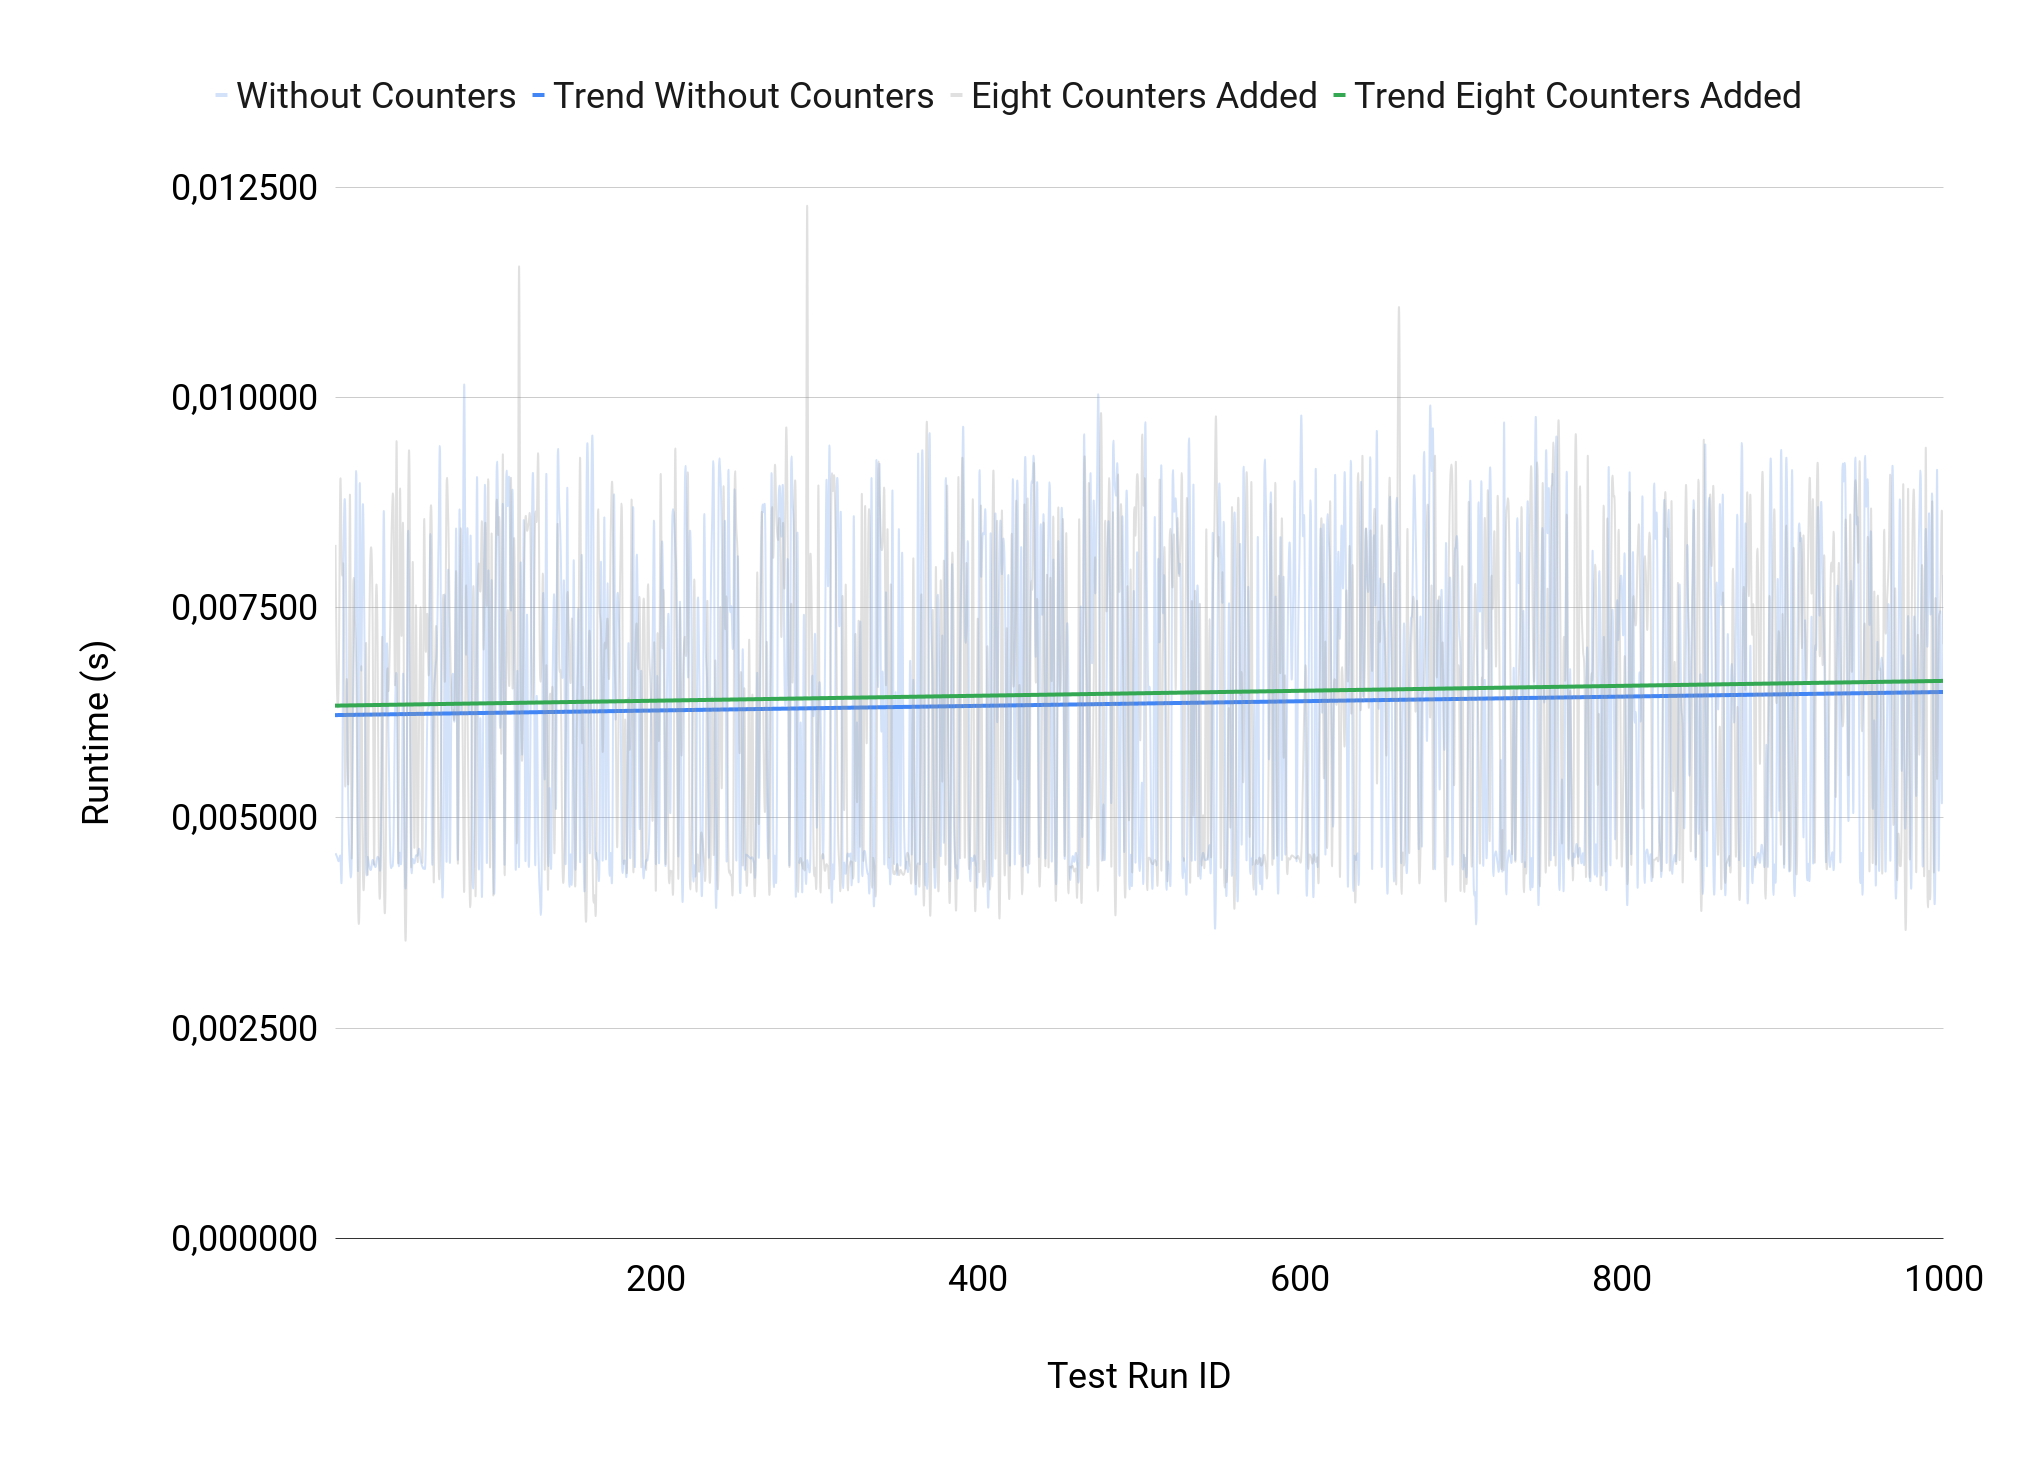
\includegraphics[width=1\textwidth]{graphics/e_forloop_comparison.png}
  \label{fig:e:forloop_comparison}
\end{figure}

\subsection{Varying Loop Runtimes}
First, the runtime of the \VARYINGLOOP~\ref{lst:e:perf_forloops} application will be examined, focusing on the times measured with the \CHRONO library, since \emph{gnu-time} can only achieve an accuracy of \SI{0.01}{\second}. For this reason, only the inserted performance counters can be examined in this analysis and the \lstinline{print()} function can be disregarded for the time being. The objective is to identify the difference in runtimes between the two program variants and to consider the time added per inserted performance counter.

The runtimes of each run performed on the AMD Ryzen test environment can be seen in Figure~\ref{fig:e:forloop_comparison}. The average of the durations of all runs without added performance counters is  \SI{16300}{\micro\second}, whereas the runtime after adding the performance counters is around \SI{16480}{\micro\second}, which in result is a deviation of \SI{180}{\micro\second}. In this example, a total of four \MEASUREPAIRS were recorded, whereby one measures the total running time and the other three the individual \lstinline{for}-loops. Thus it can be calculated that each \MEASUREPAIR consumed about \SI{45}{\micro\second} in this test environment. 

Figure~\ref{fig:e:forloop_environments} shows the average durations per run on the three test environments, once with counter added and once without counter added. It can be seen that on average the programs with added counters consumed \SI{0.34}{\percent}--\SI{2.28}{\percent} more time. If the increased time is calculated down to a single added performance counter, this results in a time of \SI{20}{\micro\second} for each \MEASUREVALUE taken across all environments. 

It can be stated that especially with programs that have a short runtime and only a few counters have to be added by the \TOOL, only a marginal deviation can be recognized. 

\begin{figure}[t]
  \centering
  \caption[Runtime Deviation for the \VARYINGLOOP Application.]{Runtime Deviation for the Execution of the \VARYINGLOOP Application. The diagram shows the increase in runtime in percent when eight counters are added. The test was performed on a \IMAC and a \MACBOOK and a \AMD.} 
  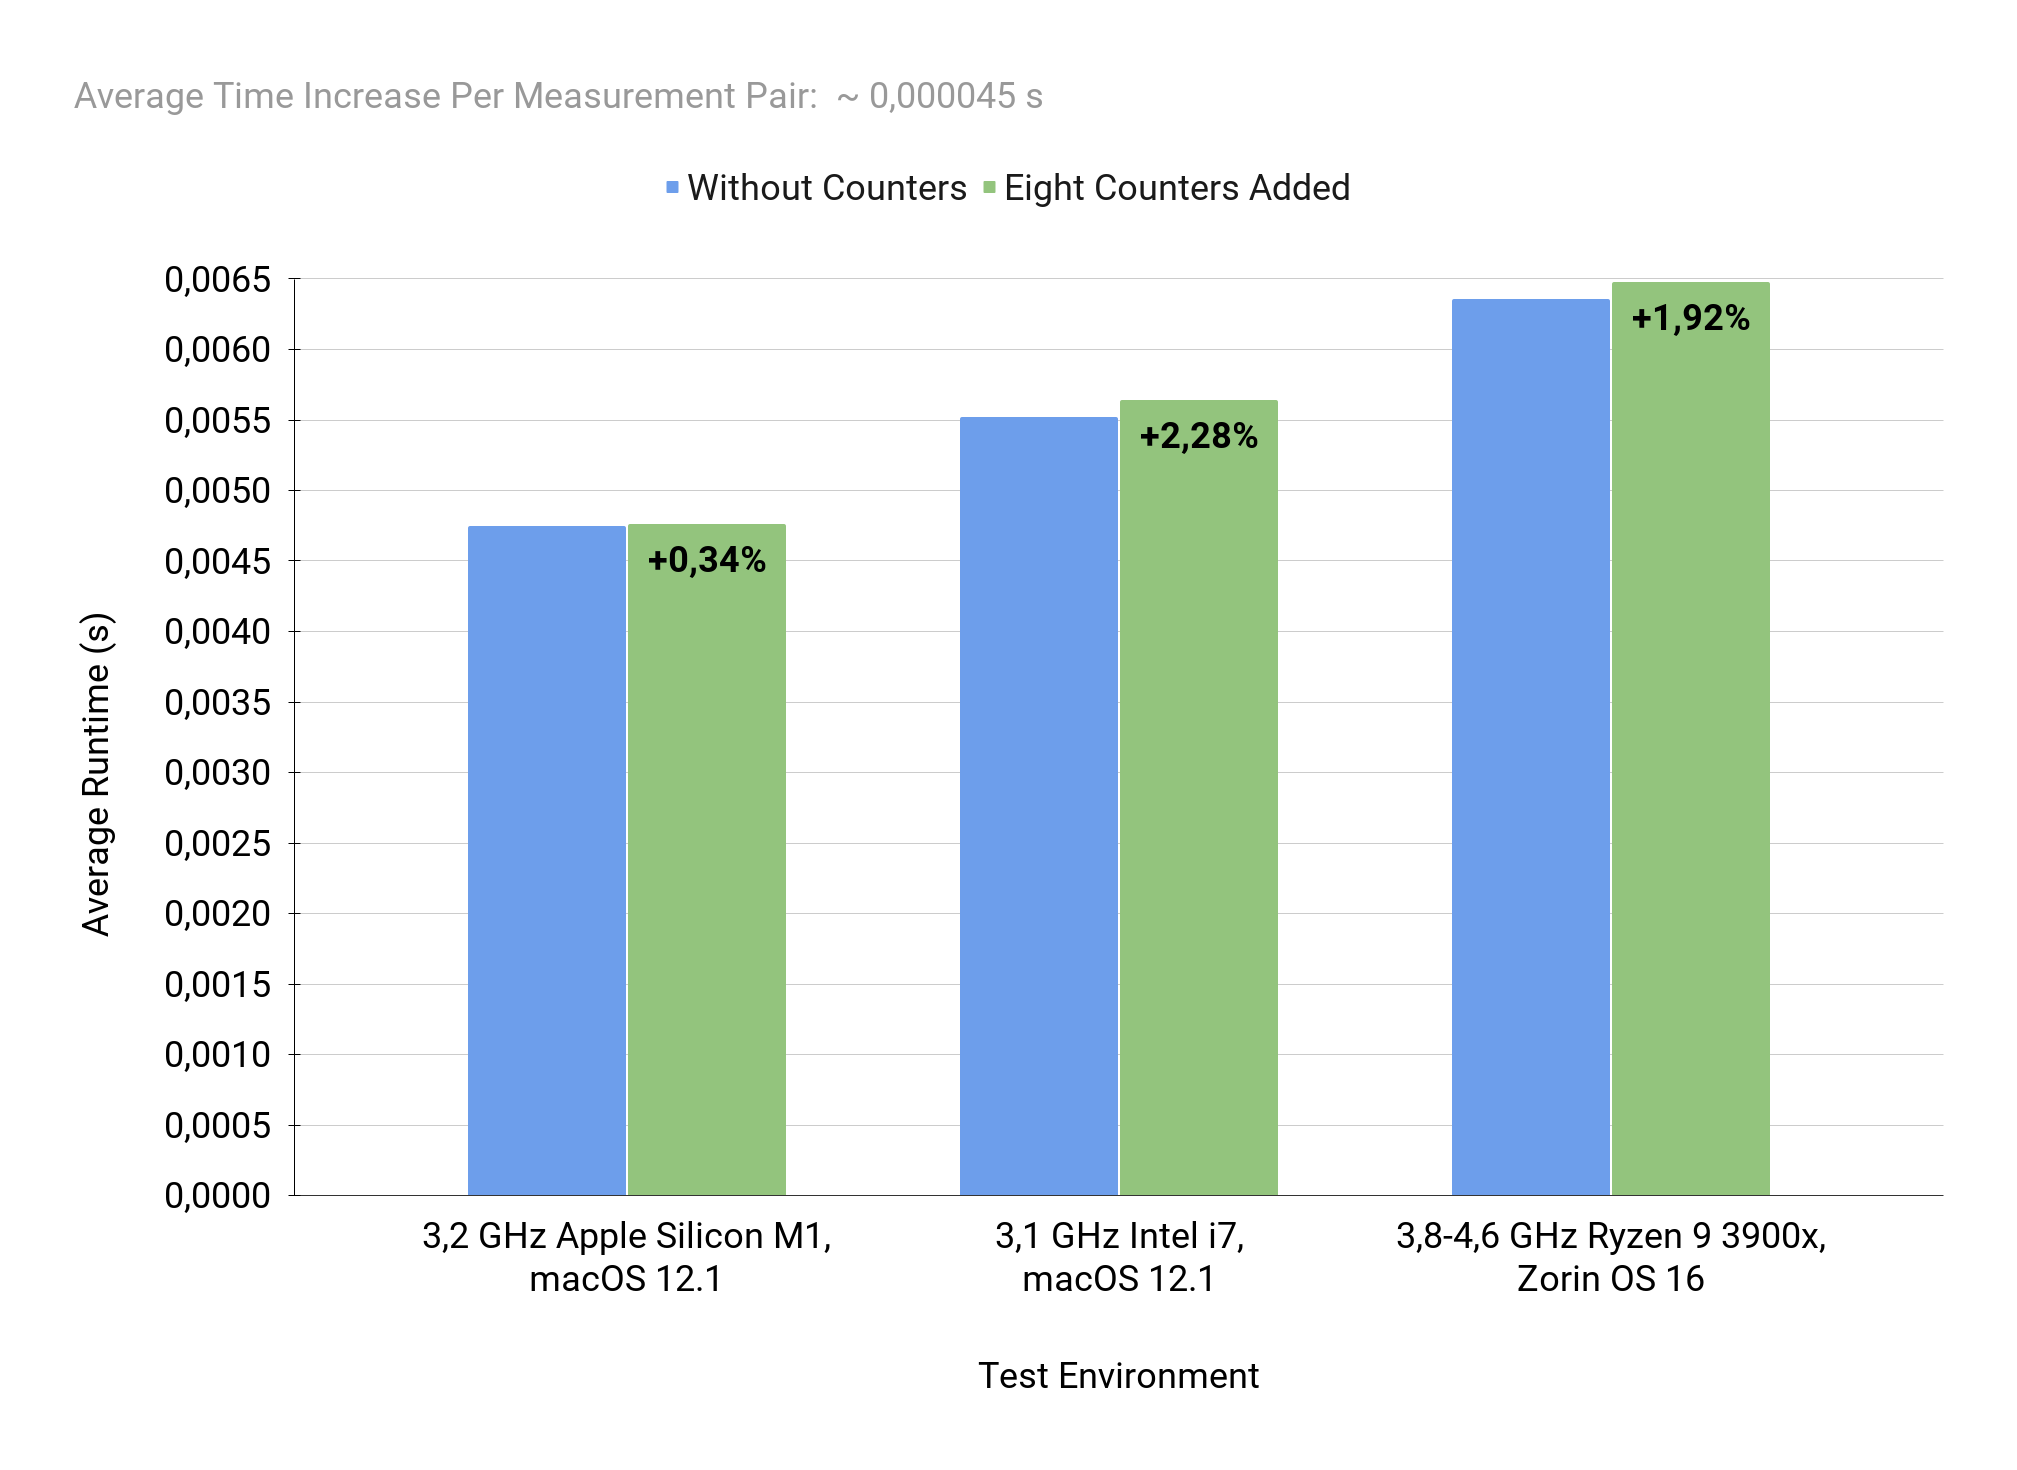
\includegraphics[width=1\textwidth]{graphics/e_forloop_environments.png}
  \label{fig:e:forloop_environments}
\end{figure}

\begin{figure}[t]
  \centering
  \caption[Runtime Comparison for the \FIBONACCI Application.]{Runtime Comparison for the \FIBONACCI Application. The runtime of the program without counters is compared to the version with eight counters added and the version with 4004 counters added. The Trend Lines Shown Represent the Average of the Runtimes Across All Test Environments. The test was performed on a \IMAC and a \MACBOOK and a \AMD.} 
  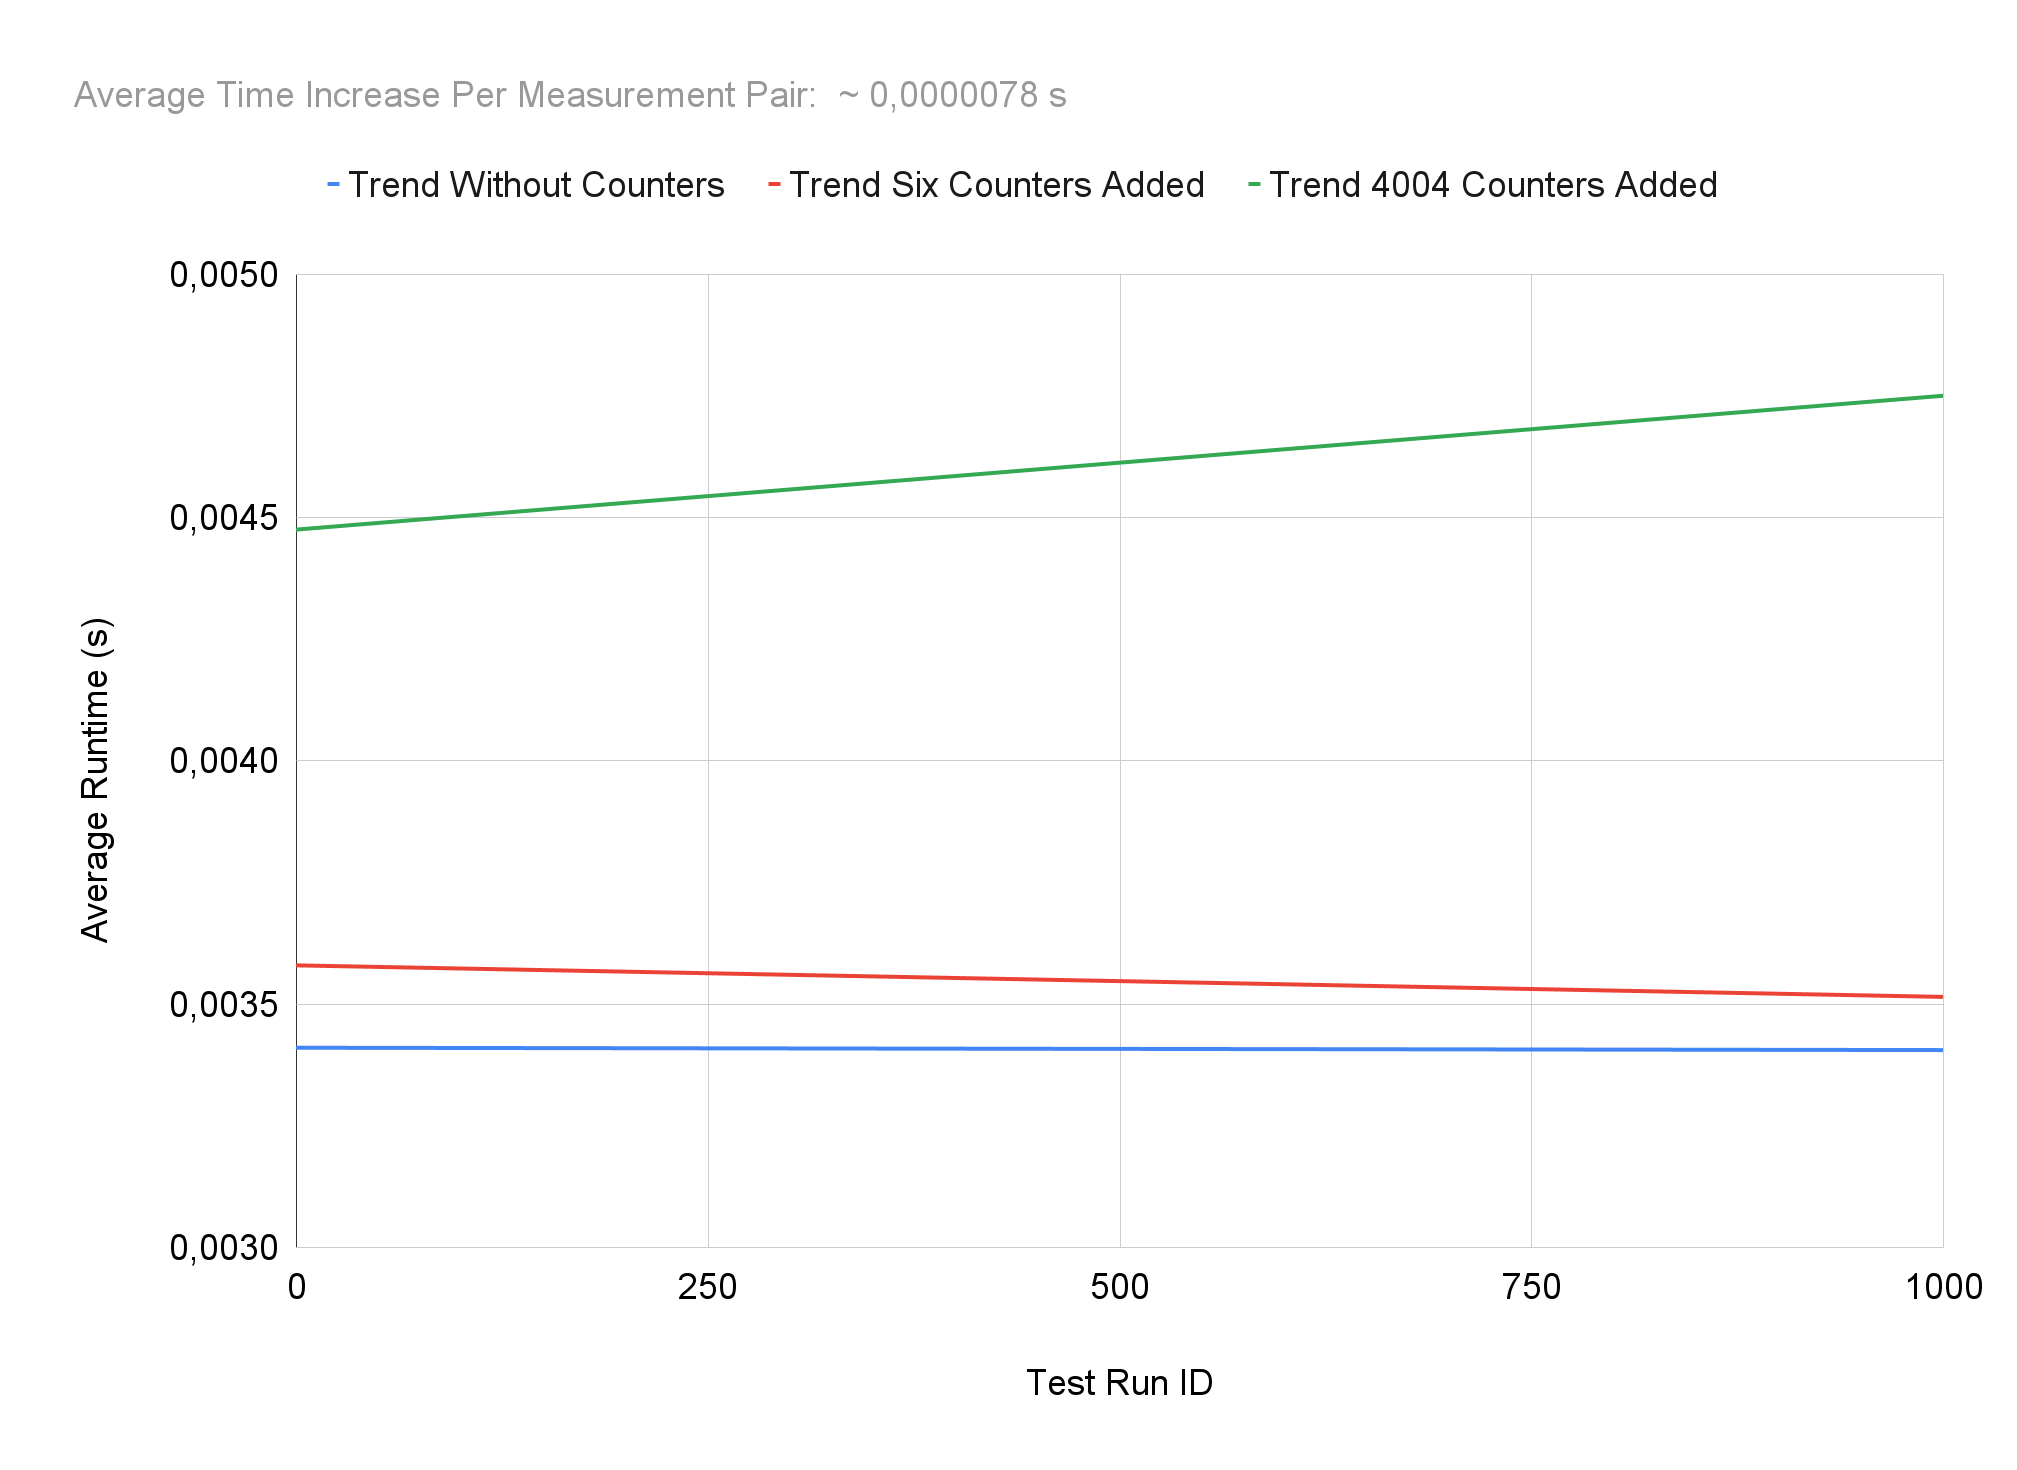
\includegraphics[width=1\textwidth]{graphics/e_fibonacci_comparison.png}
  \label{fig:e:fibonacci_comparison}
\end{figure}

\subsection{Fibonacci Sequence}
The \FIBONACCI~\ref{lst:e:perf_fibonacci} application that calculates the first thousand Fibonacci numbers will be looked at next. In contrast to the previous application, we showed in Section~\ref{sectionFibonacciCode} that two steps were needed to find the most resource-intensive part of the program. In the first step, the total running time and the duration of two single instructions were measured, which amounts to a total of three \MEASUREPAIRS or six \MEASUREVALUES recorded. In the second step, in addition to the total runtime, the runtime of the scope and two single instructions within a \lstinline{for}-loop were calculated. Since the \lstinline{for}-loop is executed exactly one thousand times and two instructions are measured within each, the total number of \MEASUREPAIRS is two thousand plus two pairs for the total and scope runtime, which amounts to 2002 \MEASUREPAIRS or 4004 \MEASUREVALUES. This example is intended to show that a distinction must be made between measurements that are performed only once and measurements that occur in a loop or a recursive function.

In Figure~\ref{fig:e:fibonacci_comparison}, the average runtimes of all environments for each run are given as trend lines. It can be seen that there is only a slight deviation between the variant without performance counter and the variant with six added \MEASUREVALUES. This difference amounts to an average of about \SI{4.11}{\percent} on all test environments. In the variant with 4004 \MEASUREVALUE recorded, on the other hand, a more significant increase in runtime of around \SI{39.22}{\percent} can be seen. It can be stated that in this example there seems to be no clear dependence between the number of \MEASUREVALUES recorded and the added runtime, since the deviations do not increase proportionally to each other. 

This behaviour can also be observed by looking at the average time increase per \MEASUREPAIR. The program version without added counters takes on average \SI{1136}{\micro\second}, the variant with six counters added around \SI{1182}{\micro\second} and the variant with 4004 counters added around \SI{1538}{\micro\second}. If we now calculate the average added per \MEASUREPAIR in this example, we get \SI{7,8}{\micro\second} per pair. However, it should be noted that a \MEASUREPAIR costs around \SI{15}{\micro\second} in the first step and only \SI{0.2}{\micro\second} in the second, although significantly more \MEASUREVALUES were recorded. This can be explained by the fact that the memory does not have to be reallocated with each loop pass, but only the current value has to be overwritten. 

Finally, the \TOTALCODEBLOCK can be considered. Although the costs of one \MEASUREPAIR is decreasing, the total time required to calculate the time of one code block is generally increasing. In the first step, the \TOTALCODEBLOCK cost around \SI{15}{\micro\second}, in the second step around \SI{100}{\micro\second}. This results from the fact that although the cost for a single \MEASUREVALUE is now lower, at the same time far more measurements are needed to calculate the time of one code block. Furthermore, it can also be stated that the execution time of the program is still very short and side effects caused by the hardware, the operating system or the time calculations of the runs can have a large impact on the final results. Consequently, the focus should shift to programs with a longer duration. Thus, we can take a closer look at the impact of the \MEASUREVALUES recorded on programs with a longer runtime.

\begin{figure}[t]
  \centering
  \caption[Runtime Comparison for the \PASSWORDGEN Application.]{Runtime Comparison for the \PASSWORDGEN Application. The Figure Shows The Average Runtime Over All Environments for Each Run. Program versions with a varying amount of added counters are compared to each other. The test was performed on a \IMAC and a \MACBOOK and a \AMD.} 
  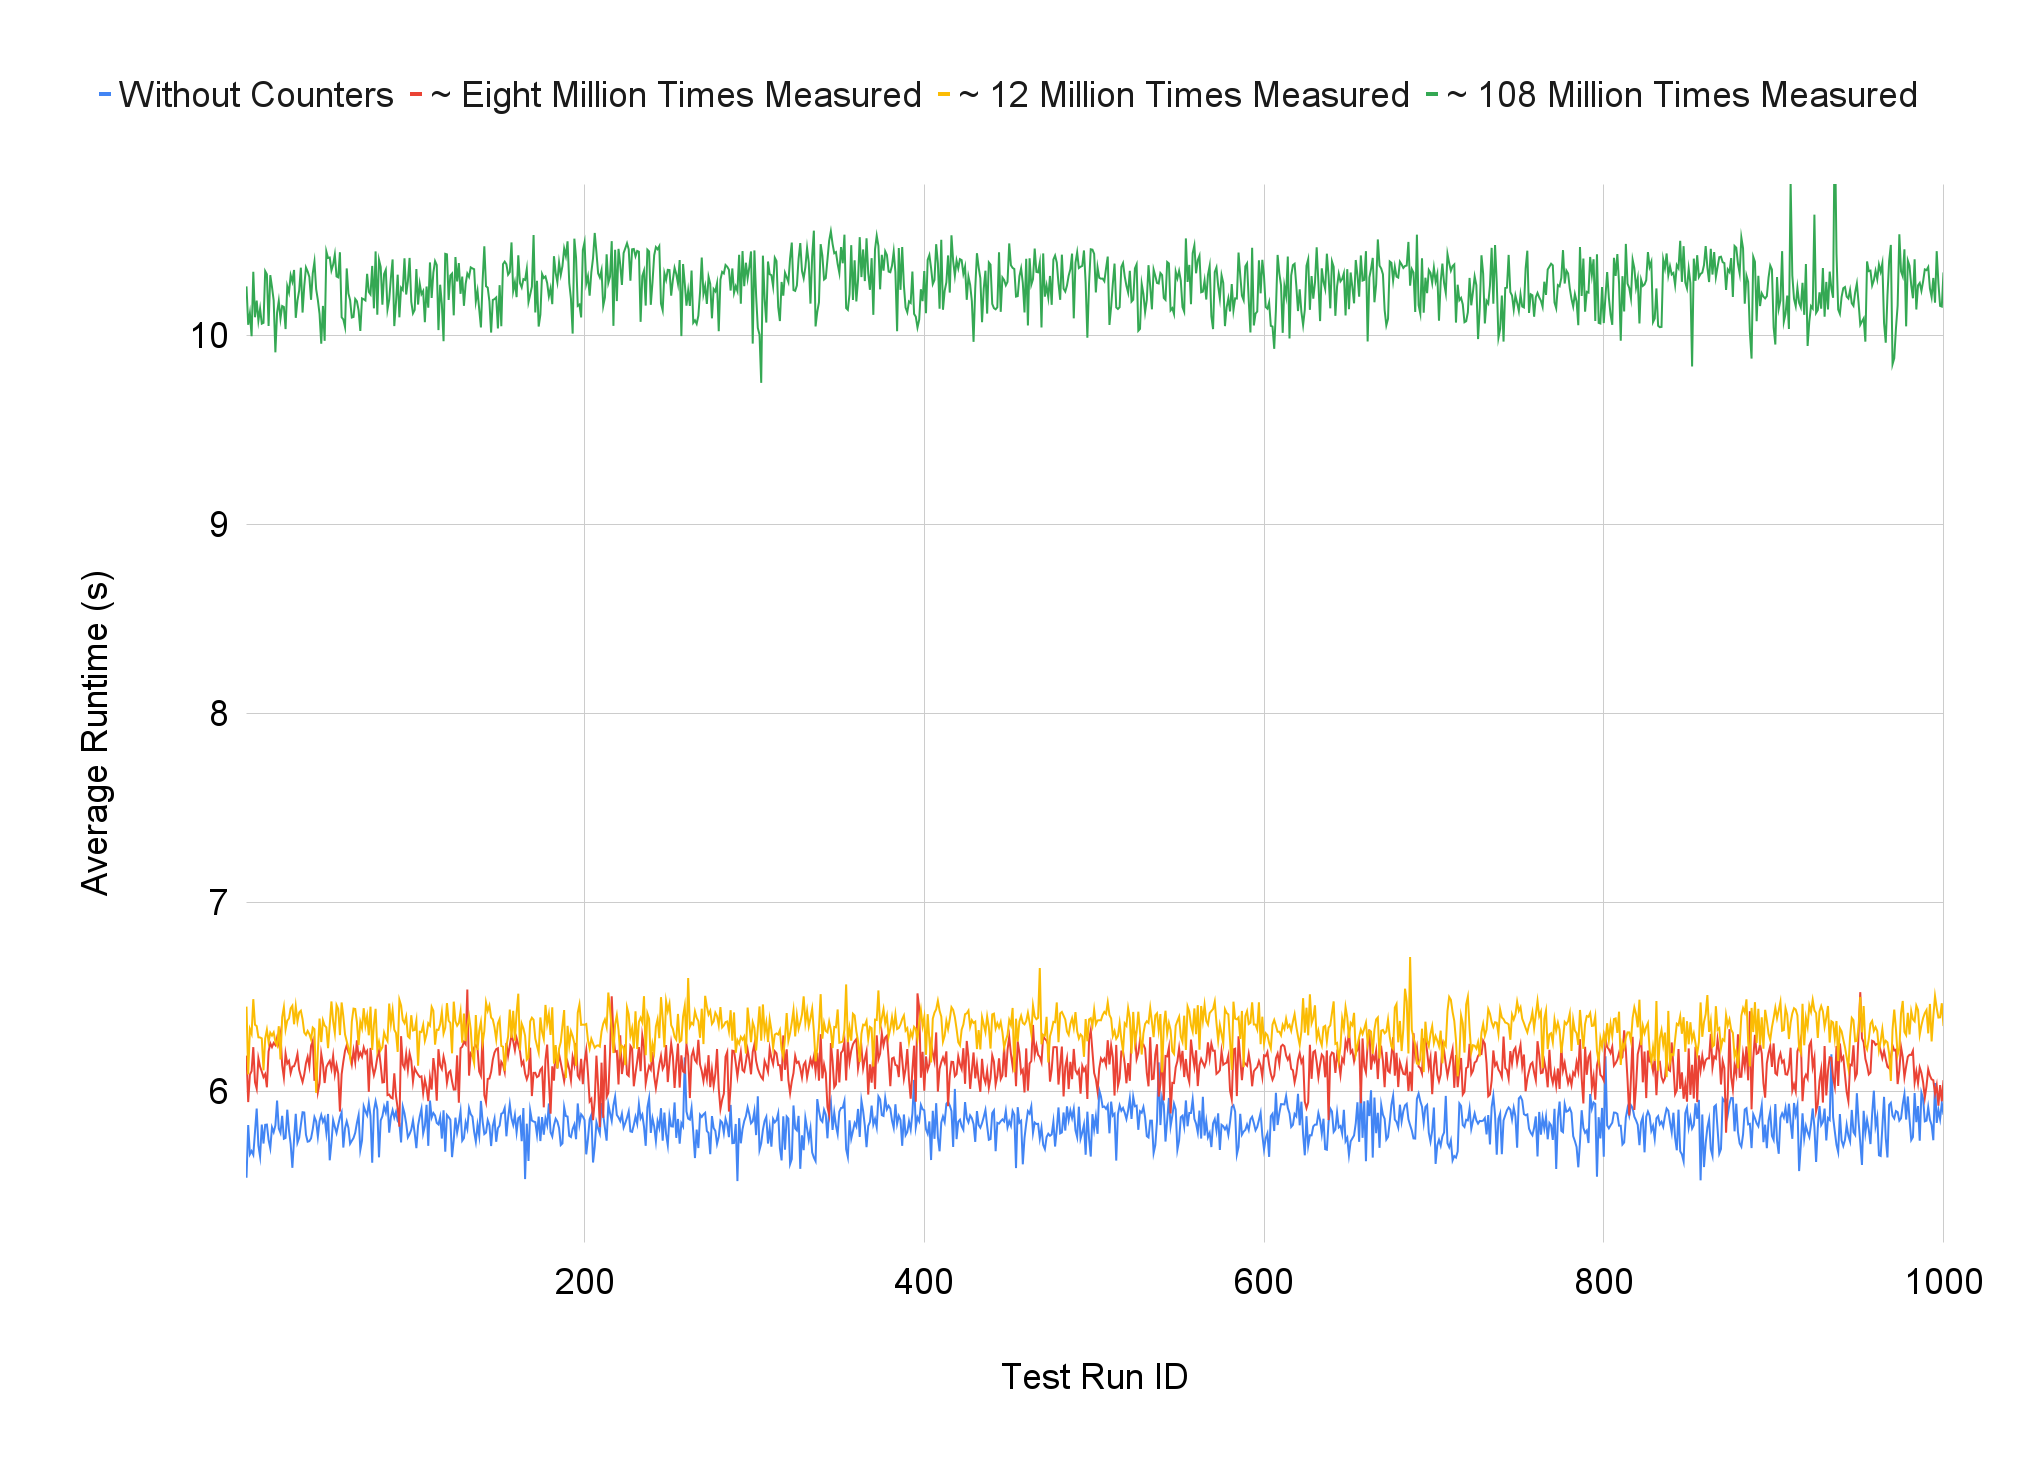
\includegraphics[width=1\textwidth]{graphics/e_password_comparison.png}
  \label{fig:e:password_comparison}
\end{figure}

\subsection{Password Generator}
The \PASSWORDGEN~\ref{lst:e:perf_passwords} application is to be examined next. We showed in Section~\ref{sectionPasswordCode} that a total of four steps were necessary in the profiling process to find the desired position in the code. In the first pass, eight \MEASUREVALUES were recorded for the time calculation of three code blocks, in the second eight million for the calculation of four code blocks, in the third fourteen million for calculating the time of two code blocks and in the last step 114 million for the calculation of three code blocks. The objective is to determine how the added performance counters affect programs with a longer runtime.

The average runtimes for each run across all test environments is shown in Figure~\ref{fig:e:password_comparison}. We have already discussed the deviations caused by a few added performance counters, so the first step is not considered for the following examples. The second step shows an increase in runtime of \SI{6.11}{\percent}, the third step an increase of \SI{10.68}{\percent} and the last step an increase of \SI{85.64}{\percent}. It can be noted that the increase scales approximately with the number of \MEASUREVALUES recorded. 

To view this effect from a different perspective, the average of the added time per \MEASUREPAIR can be calculated. The result is \SI{0.096}{\micro\second} per \MEASUREPAIR in step two, \SI{0.1}{\micro\second} in step three and \SI{0.092}{\micro\second} in step four, which amounts to an average of \SI{0.097}{\micro\second}. It can be seen that the runtime added per \MEASUREPAIR remains at approximately the same level or even decreases although more \MEASUREVALUES are taken in total. This can be explained by the fact that the allocation of memory for the individual data structure entries no longer has such a large influence on the result. In the previous example it could be seen that it has a big influence whether three or four \MEASUREPAIRS have to be allocated. However, in this application the deviation between the different numbers of \MEASUREPAIRS is negligible. 

In contrast, we want to look again at the time that must be spent to calculate the time of one code block. In the second step \SI{0.064}{\second} were spent, in the third step \SI{0.18}{\second} and in the last step \SI{1.05}{\second}. It can be seen that the \TOTALCODEBLOCK increases, since more calculations are needed to calculate the runtime of one code block. To investigate this further, the \PASSWORDGEN program will be modified so that a different number of passwords is added in each run. 

\subsection{Variable Password Size Generator}
For the \VARPASSWORDGEN Application the fourth step of the \PASSWORDGEN is to be adapted so that there is also a number of five data structure entries. This has the advantage that the difference caused by different numbers of data structure entries can be completely eliminated, since all runs have the same number of code blocks to be measured. Furthermore, the number of passwords should be randomly generated in the range from zero to two million so that any side effects caused by the hardware or the operating system can be distributed across all runs. Furthermore, the runs are now performed two thousand times to get a wider range of information. 

\begin{figure}[t]
  \centering
  \caption[Runtime Comparison for the \VARPASSWORDGEN Application.]{Runtime Comparison for the \VARPASSWORDGEN Application. The figure shows the increase of the runtime in relation to the generated passwords. The program version without added counters is compared to the version with counters and to the version with counters and \lstinline{print()} function. The test was performed on a \AMD. } 
  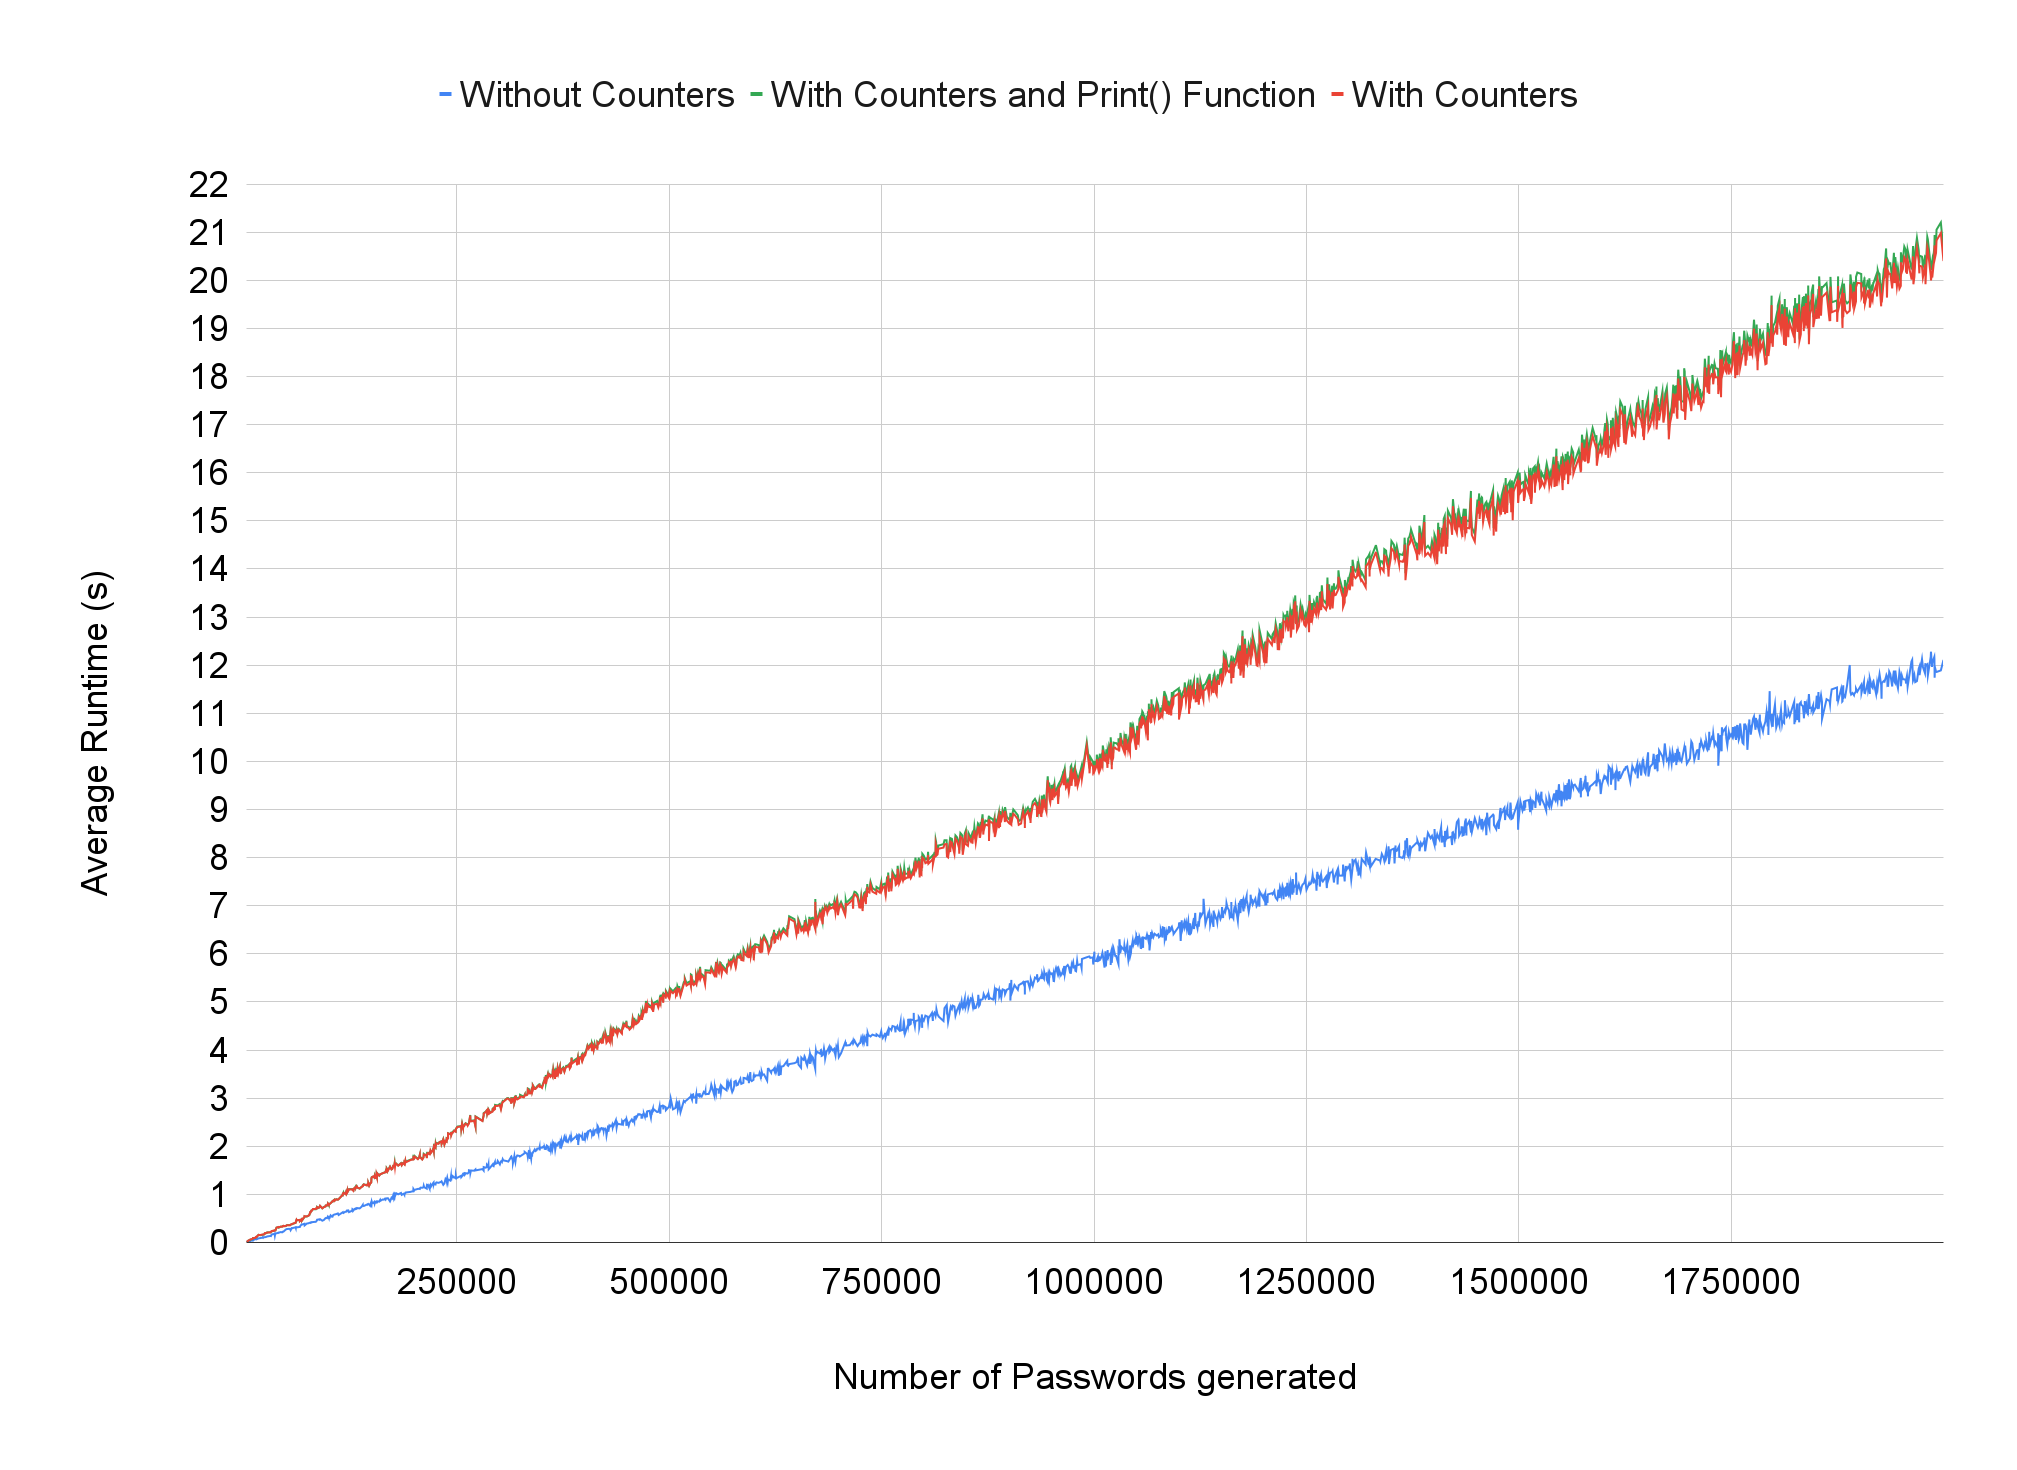
\includegraphics[width=1\textwidth]{graphics/e_variable_password_comparison.png}
  \label{fig:e:variable_password_comparison}
\end{figure}

Figure~\ref{fig:e:variable_password_comparison} shows the runtimes once with and once without added counters on the AMD Ryzen environment. In addition to the distinction between the program variants, a differentiation is now also made between the runtime of the counter itself and the runtime of the \lstinline{print()} function. On average, for five measured code blocks, the runtime of the \lstinline{print()} function is \SI{0.04}{\second} per run. Since in this example only a variable number \MEASUREVALUES are recorded, but the number of code blocks which runtime statistic is to be printed remains the same, the runtime of the \lstinline{print()} function does not change, but add a constant value to the total runtime. This is the case because the calculations of the runtimes of a loop are already made within the \lstinline{startEvent()} function, thus an enormous amount of resources can be saved since two separate timestamps do not have to be stored for each loop run. It can be noted that the runtime of the \lstinline{print()} function can only be increased by adding more code blocks to be measured, but adding single \MEASUREVALUES has no influence.

Furthermore, it should be calculated for all runs over all environments how much runtime is allocated to one \MEASUREVALUE. For this purpose, the total runtime can be divided by the number of performance counters used in this run. For the data of the program variant without inserted counters, the number of counters that would have been consumed can be calculated by scaling the number of passwords. An average value of \SI{0.06}{\micro\second} per \MEASUREVALUE can be calculated over the six thousand collected measurements. It can therefore be stated that a \MEASUREPAIR in this example costs around \SI{0.11}{\micro\second} of running time. Comparing this value with those of the previous examples, especially the second step in the \FIBONACCI program and step two to four in the \PASSWORDGEN application, it is noticeable that the deviation from the values calculated of these examples is very small. However, an average of \SI{1.3}{\second} was now spent calculating one code block. In the following we will compare the results of all programs in detail.

\begin{figure}[t]
    \centering
    \caption[Time Per \emph{Measurement Value} Comparison for Various Test Cases.]{Time Per \emph{Measurement Value} Comparison for Various Test Cases. The diagram shows the average time taken to record a \MEASUREVALUE. The \MEASUREVALUES calculated in the previous examples are compared to each other.}
    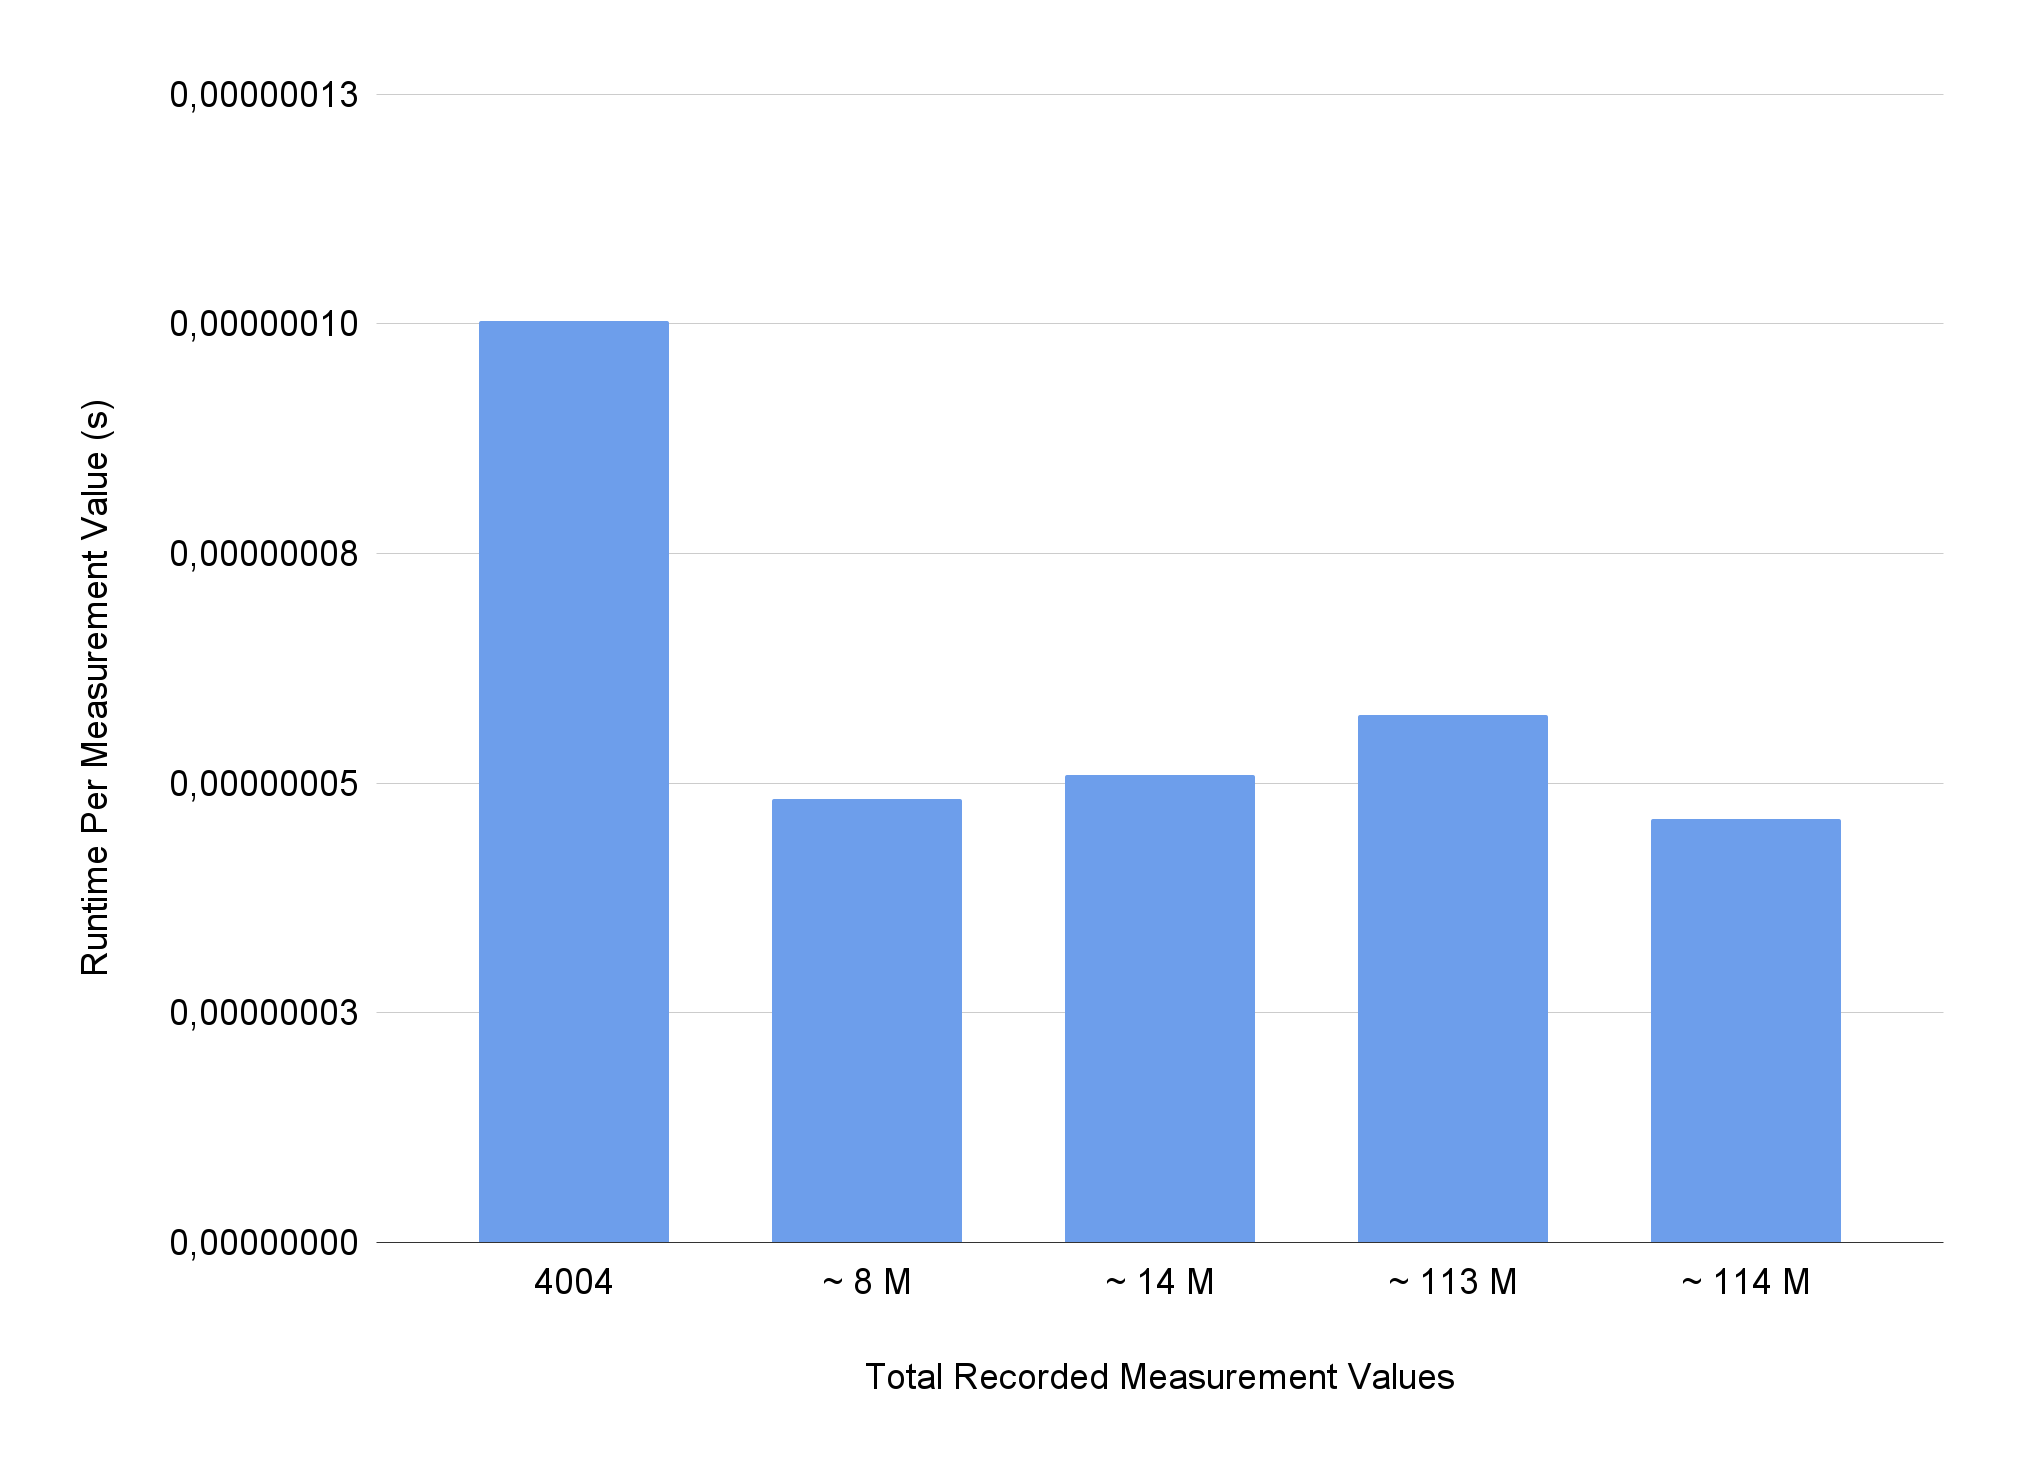
\includegraphics[width=\textwidth]{graphics/e_conclusion_per_counter.png}
    \label{fig:e:conclusion_per_counter}
\end{figure}
 
\subsection{Time Per Measurement And Total Overhead Per Code Block}
All values found for the runtime generated by one \MEASUREVALUE and the \TOTALCODEBLOCK of the various programs should be examined. Figure~\ref{fig:e:conclusion_per_counter} lists the additional times required per \MEASUREVALUE. It can be seen that this value stabilizes as more times are measured. The sum of the five considered values is \SI{0.06}{\micro\second}. Figure~\ref{fig:e:conclusion_per_array_entry} shows the \TOTALCODEBLOCK for all examples. These times increase as more \MEASUREVALUES are needed to calculate one code block. For the value calculated per \MEASUREVALUE, it can be said that it will not decrease further, but the \TOTALCODEBLOCK may greatly increase if more timestamps are measured and calculated.

\begin{figure}[t]
    \centering
    \caption[\emph{Total Overhead Per Code Block} Comparison for Various Test Cases.]{\emph{Total Overhead Per Code Block} Comparison for Various Test Cases. The diagram shows how much overhead was generated by the measurement of one code block. The \TOTALCODEBLOCK calculated in the previous examples are compared to each other.}
    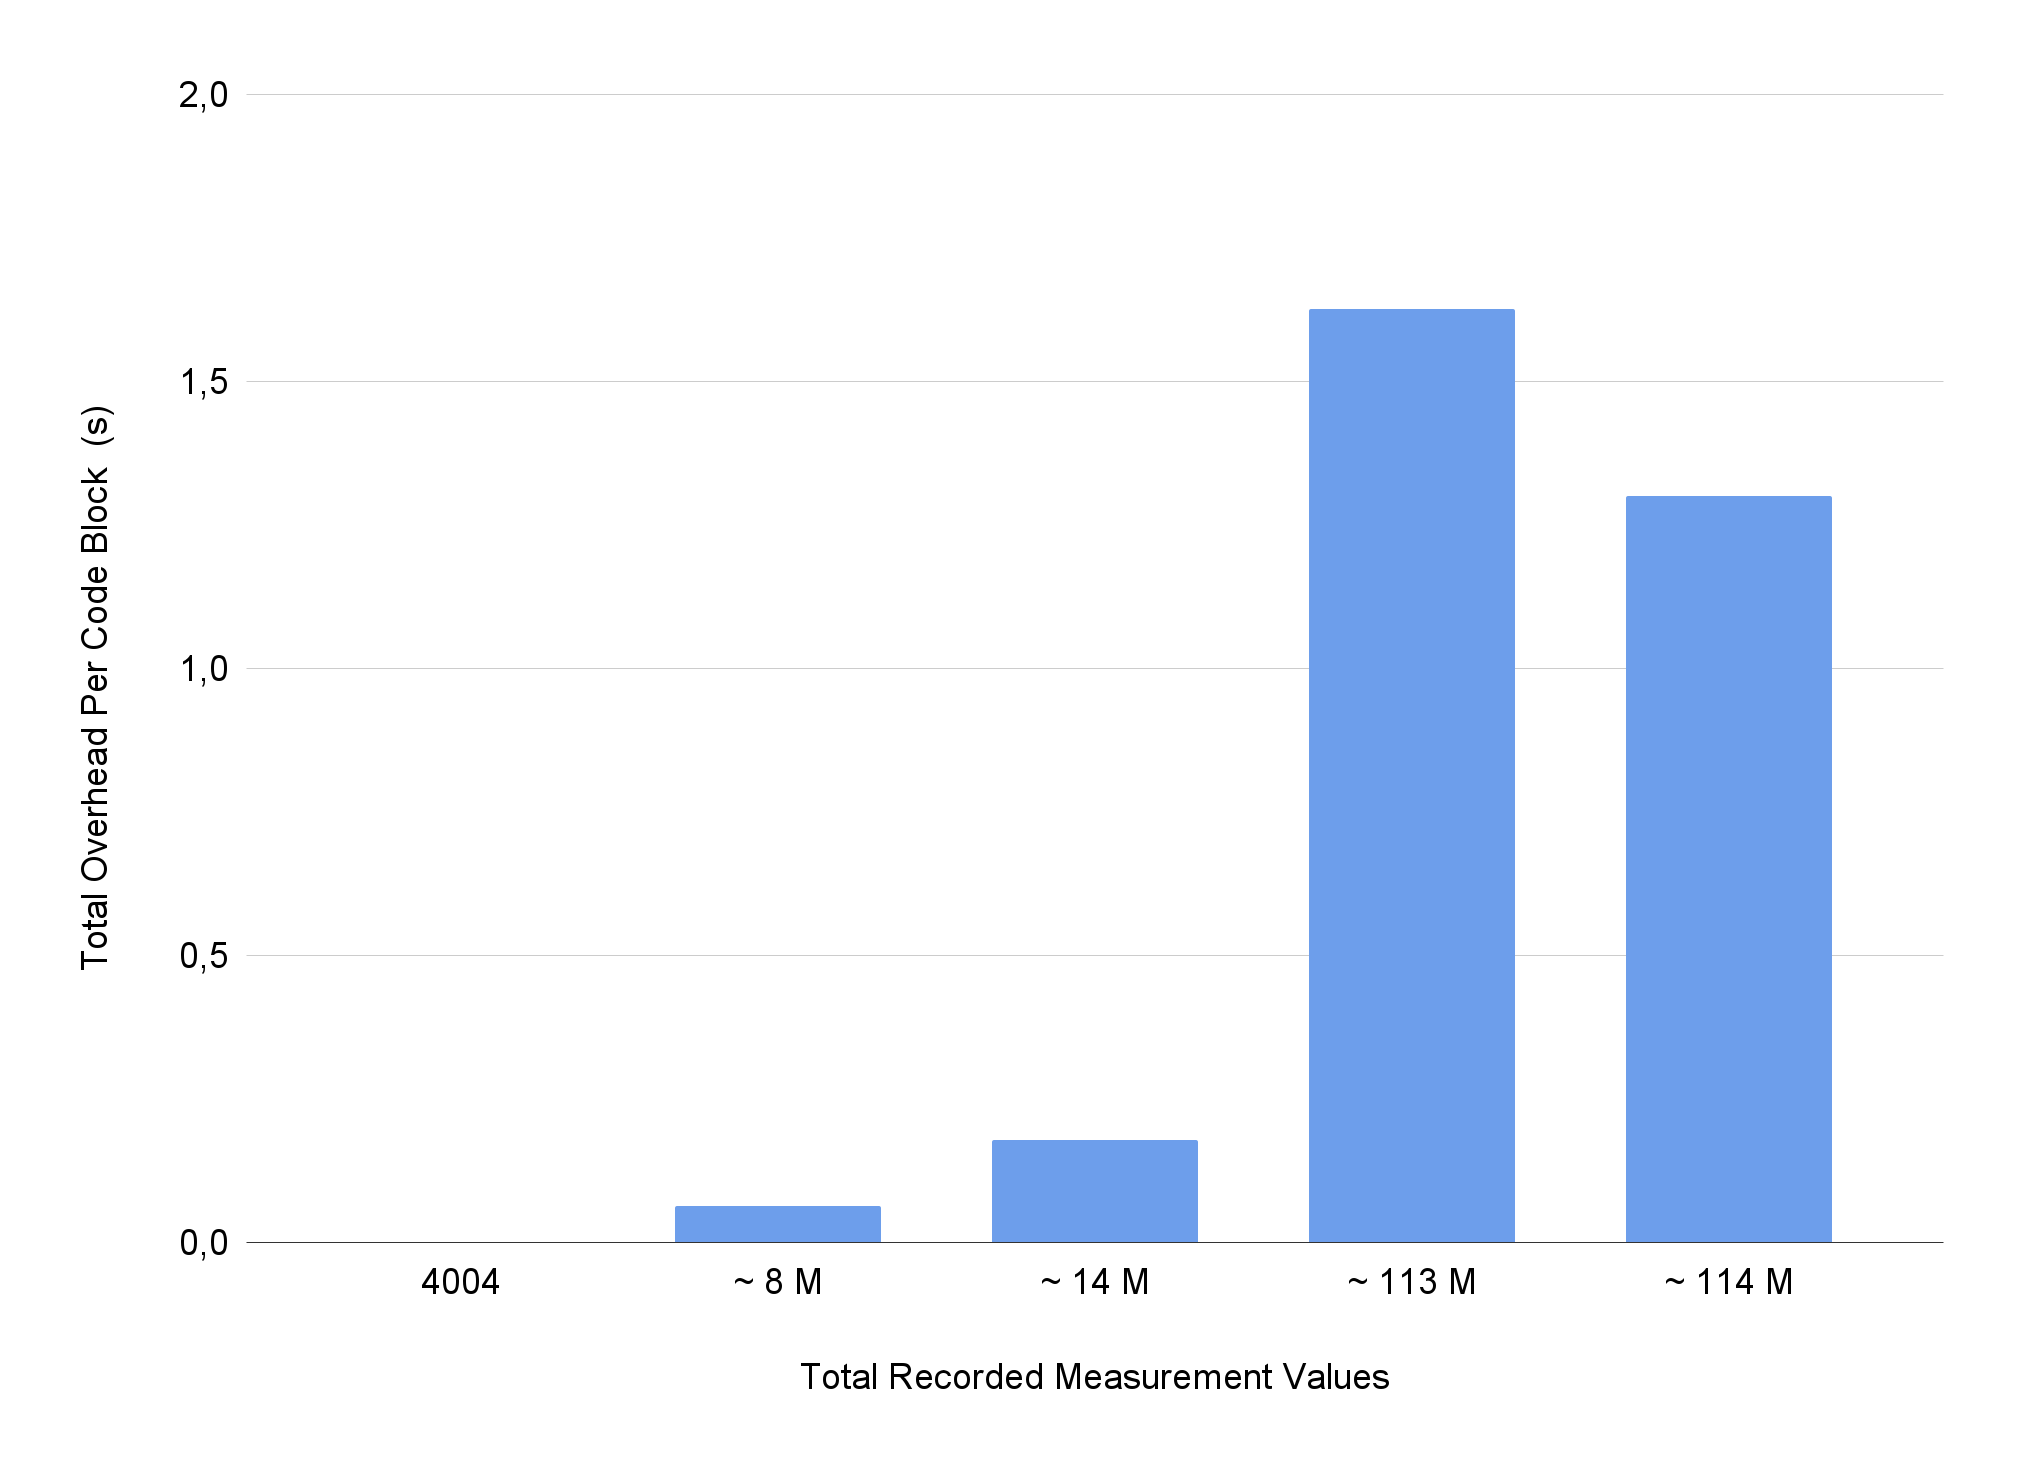
\includegraphics[width=\textwidth]{graphics/e_conclusion_per_array_entry.png}
    \label{fig:e:conclusion_per_array_entry}
\end{figure}

In conclusion, it can be stated that the performance of the tool depends on three parameters. The first one is the number of code blocks to be measured, which can be neglected especially if many measurements are carried out. The second parameter is the \TOTALCODEBLOCK. This value rise when more readings are needed to measure a single code block. The last parameter is the time taken by \MEASUREVALUE. It was found that this value stabilizes with a large number of measurements and drops below \SI{0.1}{\micro\second} after about a thousand measurements have been taken. It should also be noted that although the execution time of the program increases by inserting further measurements, the quality of the profiling process is not necessarily affected. On one hand, the \TOOL recognizes about half of the additional time consumed, even without further prediction models applied. On the other hand, the proportion of time consumed on one level enlarges evenly for all instructions, which means that statements can still be made about the most resource-intensive part of an application.  

\begin{figure}[t]
  \centering
  \caption[Prime Number Comparison for the \PRIME Application.]{Prime Number Comparison for the \PRIME Application. The diagram shows the ratio of calculated prime numbers to added performance counters. The runtime of all environments is compared to each other. The test was performed on a \IMAC and a \MACBOOK and a \AMD.} 
  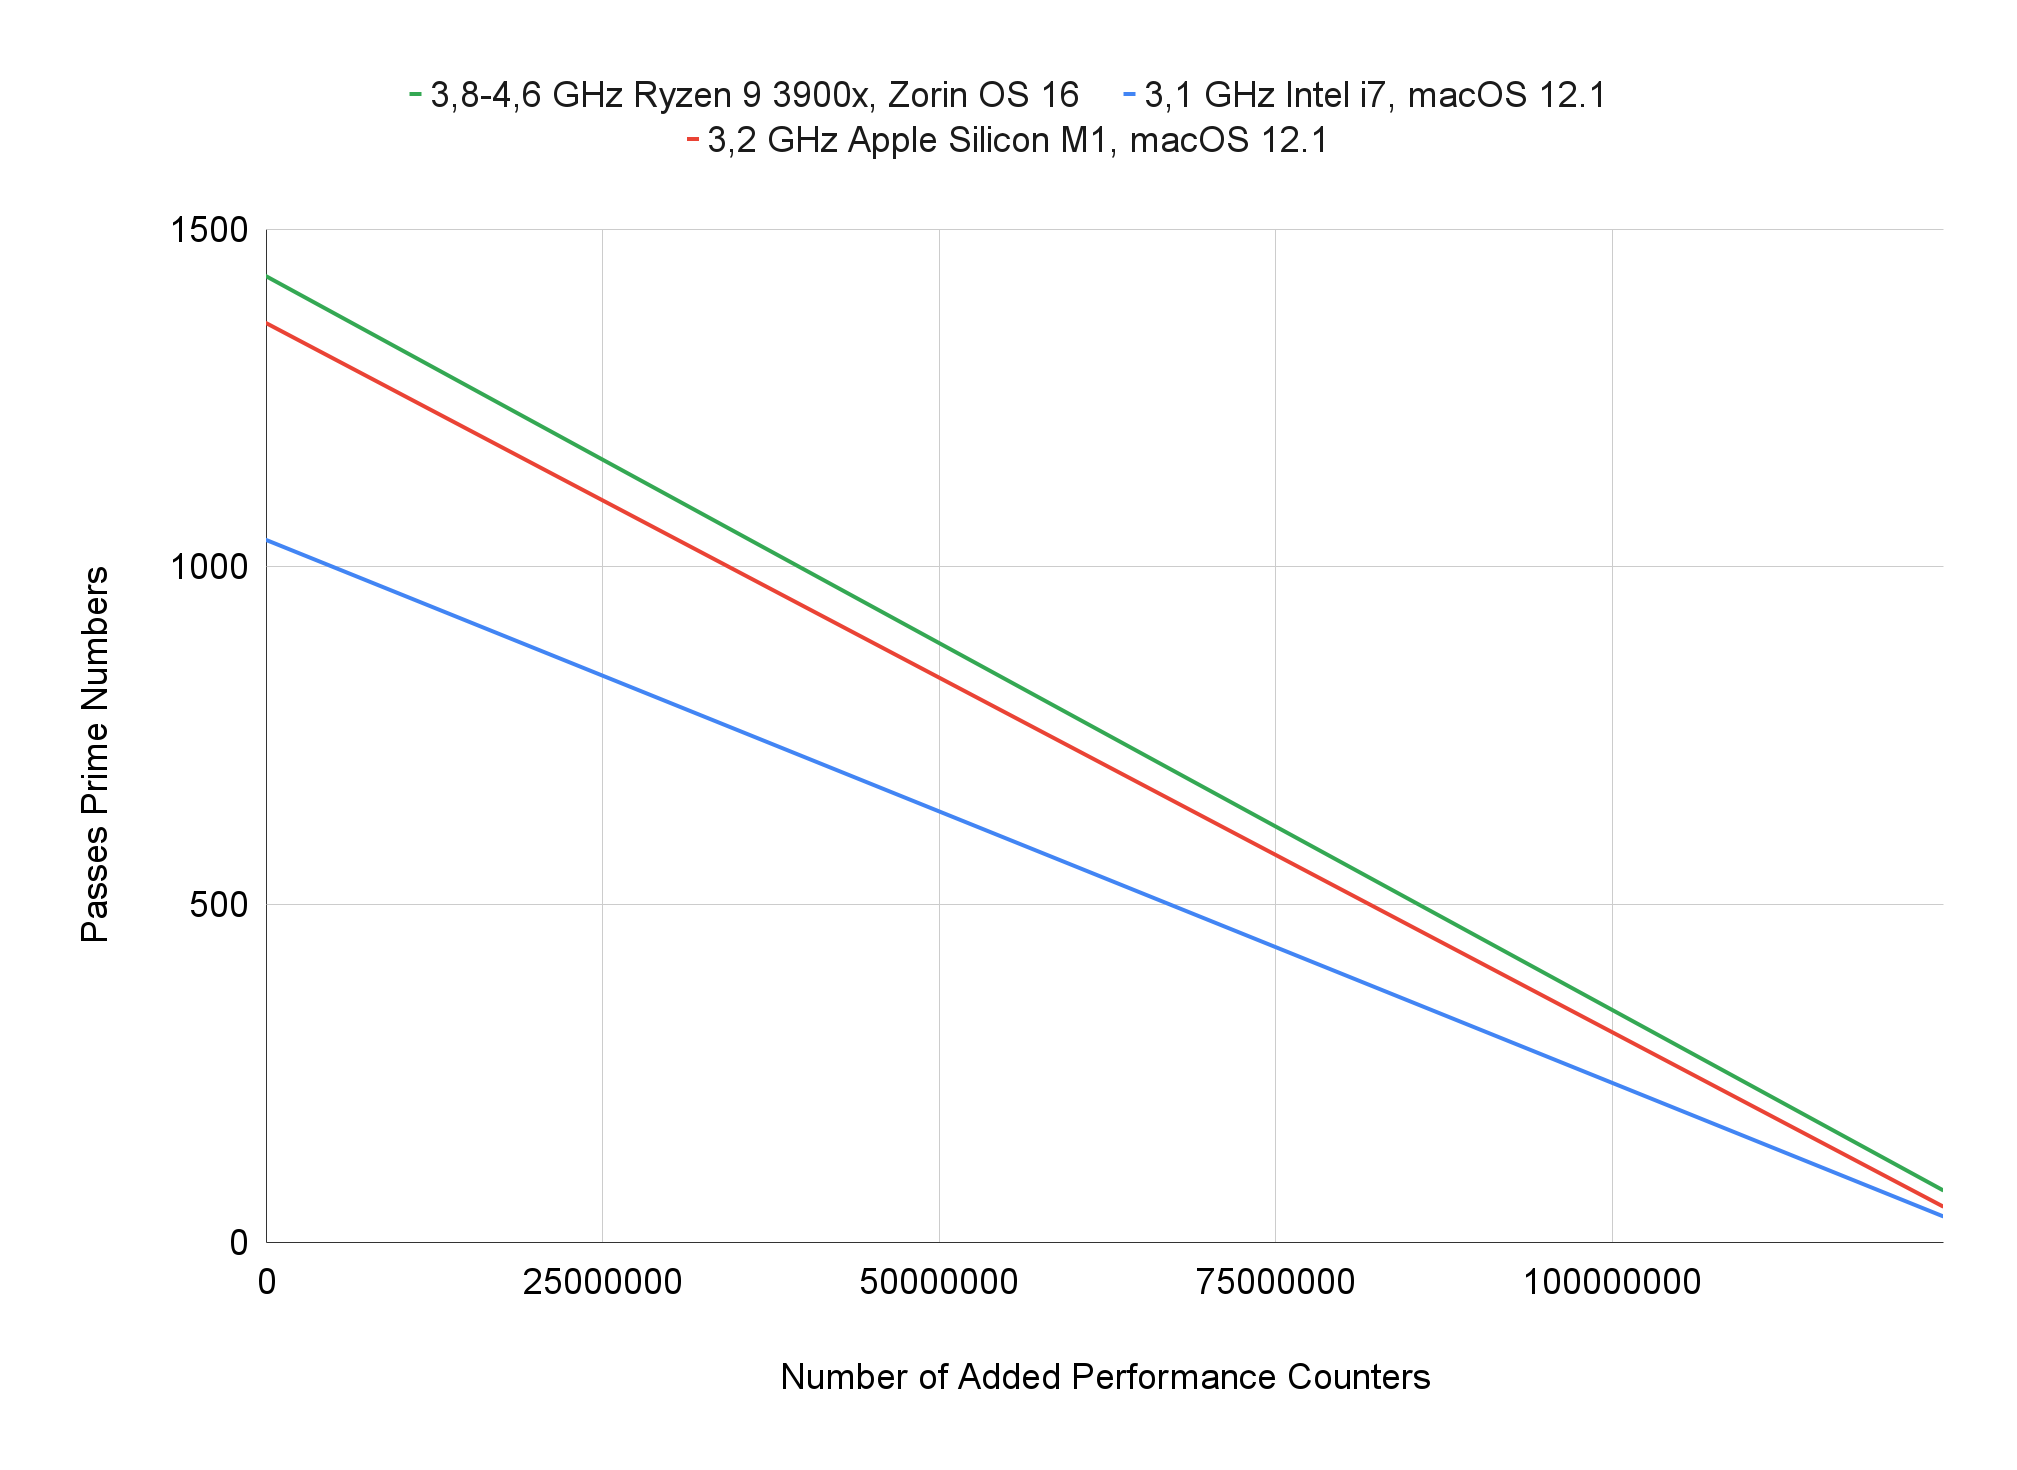
\includegraphics[width=1\textwidth]{graphics/e_prime_comparison.png}
  \label{fig:e:prime_comparison}
\end{figure}

\subsection{Prime Benchmark}
After all statements about the added time of the \TOOL have been made, the \PRIME~\cite{PrimeBenchmark} program will now be considered. In this example, no runtimes were measured, but rather calculated prime numbers. We showed in Section~\ref{sectionPrimeCode} that in order to reach the most resource-intensive part of the application, a total of six steps were required, whereby a different variable number of counters were inserted in each run, as this was dependent on the performance of the current run. In the first step, four \MEASUREVALUES were recorded, in the second, an average of 10241, in the third, a mean of 5105, in the fourth, approximately 1.2 million, in the fifth, an average of 0.8 million, and in the last step, an mean of 91 million. This test is particularly important to show that the \TOOL can also be used for any third-party application.

Figure~\ref{fig:e:prime_comparison} shows the results of the test on all environments, with a linear regression trend calculated across all steps. Since the first five readings are very close to each other, the values of these runs have to be looked at separately, but in general it can be seen that fewer prime numbers could be calculated by adding the counters. In the range from zero to ten thousand inserted counters, an average of 1280 prime numbers were calculated. In steps four and five, around 1260 primes were calculated in a range of 0.8--1.2 million inserted measurements. In the last step, with 91 million counters, only 56 prime numbers could be calculated. This can be explained by the fact that the time for the calculation of the prime numbers was not changed, but more counters were inserted, thus the time for the actual calculation approaches zero. 

For this specific application, it can be stated that the first five steps can be carried out without any problems, and only a slight performance drop can be detected. In the last step the calculation of the measured values takes more time than the calculations of the prime numbers themselves, whereby the performance drops enormously. Since a fixed runtime is used in this example, an infinite number of counters cannot be inserted, because at some point the profiling will take more time than the actual calculation of the prime numbers. However, we still succeeded in finding the most resource-intensive part of the program in Section~\ref{sectionPrimeCode}, since we were able to determine which part of the calculation takes the longest time, even when calculating only a few prime numbers.       % Use Cases, Performance Analysis
% Conclusion %
\chapter{Conclusion}
\label{chapter6}
In this thesis, an application was presented that enables \roismall in single-threaded \CPP programs to be automatically wrapped with performance counters to find performance bottlenecks in the source code. This was achieved by first developing a concept for traversing the \CLANG \astsmall and categorizing individual nodes. Afterwards, the functionality of the program was determined and a recursive model for the hierarchical traversal of the levels was found. Having worked out all the basic concepts, we took advantage of the \CLANG infrastructure by using the \LIBTOOLING library to develop a \CLANG tool that fulfilled our requirements. When developing this tool, we looked at how the concepts could be used to insert performance counters in the correct places in the source code. The developed program could then be used to test four applications of different complexities and runtimes for performance bottlenecks. This showed the workflow of the profiling process with this tool and proved that a resource-heavy instruction could be found in each program. Furthermore, we were able to perform a detailed overhead analysis by running each variation of the applications a number of times. In the process, we found out how much time is added by a counter and which parameters have to be taken into account when using the tool. 

\subsection{Limitations}
The implementation of the tool at this stage is limited by several constraints that were not addressed in the research question. First, it must be mentioned that the tool was developed to profile \CPP applications, but not \C or \OC. \CLANG also offers infrastructures for traversing other languages from the \C programming language family and thus the tool could be adapted based on the concepts created. To include other members of the \C language family, for instance, an additional parameter could be created for the tool, with which the user can specify which programming language is to be transformed. The file extension could also be used to determine which programming language is involved. Depending upon the language in which the input program is written, further case distinctions could be added subsequently, which address concrete characteristics of the different languages. As an example the \lstinline{CXXMemberCallExpr} can be considered. This class exists in the object-oriented language \CPP, but it is not found in an \astsmall of the \C language, which means that a case distinction would be necessary.

Another limitation we have decided in the course of the work is that not all classes that are defined in the \CLANG \astsmall are recognized separately by our tool. In this work, we have chosen a number of classes with which a variety of applications can be transformed. Further classes can be added however as desired to the present implementation. To achieve this it is necessary to consider other classes of the \astsmall provided by \CLANG and determine whether they are \LEASTAS or \PARSTAS. The existing case distinctions in the current implementation can easily be extended with new class queries. 

It should also be noted that the tool has only been applied and tested on single-threaded applications. The concepts developed can also be used for multi-threaded applications, but further special cases must be considered in more detail. Due to the concurrent processing of the instructions, it must be ensured that the data structure that manages the runtimes is synchronized, or that there is a separate storage for each thread, which is reassembled at the end of the application. 

Finally, it should be mentioned that the overhead analysis that is passed on to the user in addition to the statistics was not part of the research objective. Nevertheless, we succeeded in correctly allocating about half of the overhead without the implementation of additional calculations or predictions about the running times of the counters added. In order for the tool to be able to filter out the generated overhead even better, an algorithm could be designed, for instance, that determines how much overhead is generated in total based on the already correctly assigned share of overhead and on historical data. Thus, it would be possible to determine even more precisely how much runtime each code block really consumed.       % Limitations, Future Work


\backmatter

% Use an optional list of alogrithms.
%\listofalgorithms
%\addcontentsline{toc}{chapter}{List of Algorithms}

% Add an index.
%\printindex

% Add a glossary.
%\printglossaries

% Add a bibliography.
%\bibliographystyle{alpha}
%\bibliography{intro}

\bibliographystyle{ieeetr}
\bibliography{intro}

\end{document}